% !TeX root = doc.tex

\yinipar{M}odel reduction can be likened to digital-media compression.  We rarely work with images, video, or audio files or streams at their original resolution;  that usually requires more computing power, memory, or bandwidth than we have available.    Instead, we use lower resolution approximations that are ``good enough'' for our purposes.  We compress the data.  Significant data compression is generally lossy, meaning the reduced data contains less information than the original in some sense, which is observed as a reduction in quality.   Even as available memory and computation power increase, we continue to have problems that require more power or memory than we have.   

\smallskip
Model order reduction (MOR) is a kind of compression.   A mathematical model is a description of a working thing, a system.  We will address models of a very specific format, namely the system \eqref{eq:ds1}, but theoretically model reduction can be applied to a model of any working thing whose behavior over time can be observed and influenced (i.e. has output and input).   We seek a simpler description of that thing while preserving its behavior in response to various inputs.  Order reduction of systems of differential equations like \eqref{eq:ds1} has its origins in systems and control theory, where it has been applied to automate processes.   If the model correctly predicts a system's response to given input, we can use the model to determine how to efficiently control or influence the system.  An early example of modern model reduction is \cite{modaltrunc} from 1966.  Davison introduces the MOR method now known as modal truncation,               
\begin{quotation}\itshape
Often it is possible to represent physical systems by a number
of simultaneous linear differential equations with constant coefficients,
$\dot{x}=Ax+r$ but for many processes (e.g., chemical plants, nuclear reactors), the
order of the matrix $A$ may be quite large, say $50\times50$, $100\times100$, or even $500\times500$. It is difficult to work with these large matrices and a means
of approximating the system matrix by one of lower order
is needed. A method is proposed for reducing such matrices by constructing a matrix of lower order which has the same dominant eigenvalues and
eigenvectors as the original system.
\end{quotation}

Of course the large systems we work with today are much larger.  At the time of this writing, Krylov subspace methods are being used for systems on the order of $N=10^9$.   Krylov subspace methods are particularly suited for working with systems that are too large for other methods, many of which are quite elegant.  The reason why is that the only large matrix operation required is a sparse matrix multiplication (more correctly a sparse solve) of an order $N$ system.  If $N$ is large enough, there is not much more we can do. 
    
Krylov projection methods for working with large matrices have been around for a while, and are even claimed to be in the top 10 most important  classes of algorithms of the 20th century \cite{top10alg}.  
The first Krylov subspace projection method for model order reduction was PVL (Pade via Lanczos)  \cite{PVL} developed by Feldman and Freund in 1995.  Prior to that, Krylov methods were very successful in
\begin{itemize}
\item approximating eigenvalues of large matrices,\cite{lanczos,arnoldi} circa early 1950s,  
\item approximating the solution $Ax=b$ to  large sparse systems 
(\cite{saad1981krylov} offers a great background),
 and
\item approximating matrix function multiplications $f(A)b$ (for example $e^A b$) when $A$ is very large \cite{krylov_matfun_eval}.   
\end{itemize}

It is not a surprise then that the most successful methods for model  reduction (MOR) of a very large, sparse, descriptor system model are iterative methods, and Krylov methods in particular.     



\section{Model Order Reduction via Subspace Projection}
         Our basic problem is to approximate the ($N$-dimensional) \index{LTI system!descriptor system} \emph{Linear, Time Invariant (LTI) Descriptor System}
         \begin{equation}
         \begin{aligned}
                \E\frac{dx}{dt} &=  \A x + \BB u\\
                y &= \CC^T x
        \end{aligned}
        \label{eq:ds1}
        \end{equation}      
with a system that is realized by smaller matrices $\A_n$, $\E_n$, $\BB_n$, and $\CC_n$.  
The collection of constant matrices $(\A,\E,\BB,\CC)$ is called a
\emph{realization} \index{realization $(\A,\E,\BB,\CC)$ of the model} of the model. 

 A realization is not unique; one model can have multiple realizations.  However, two different systems cannot have the same realization.  If the model is of a circuit the matrices $\A$,$\E$,$\BB$, and $\CC$ typically come from a circuit representation method called \index{Modified Nodal Analysis (MNA)}\emph{Modified Nodal Analysis} (MNA) \cite{MNA} and have a specific structure.  A \emph{structure-preserving}  model reduction method produces a lower order model that in in fact describes a working circuit.   MOR methods are not structure preserving in general -- the reduced internal state does not retain any physical meaning.  


The state-space realization is perhaps best understood in the context of control theory.
$\A\in\R^{N\times N}$ is called the \emph{system matrix}, and $E\in\R^{N\times N}$ is the \emph{descriptor matrix}.   $\A$ and $\E$ determine the internal state of the system in the absence of external influence.  Note that if there is no input, i.e. $u(t)\equiv 0$, and we don't care about the output $y$, \eqref{eq:ds1} reduces to the unobserved, uninfluenced system
\begin{equation}
 \E\frac{dx}{dt} =  \A x.
\label{eq:state_space}
\end{equation}
 The state-space variable $x(t)\in\R^N$ represents the internal state of the system at  $t\geq 0$ and we assume a zero initial state $x(0)=0$.  

The possibly singular descriptor matrix $\E$ makes  \eqref{eq:state_space} more general than a set of Ordinary Differential Equations $x^\prime = \A x$.  Observe that if $\E$ is invertible, the first line of  \eqref{eq:ds1} can be re-written as a set of ODEs
\[
\frac{dx}{dt} =  \E^{-1}\A x + \E^{-1}\BB u
\]
which is a different and easier to solve problem.  System matrix $\A$ may be singular as well.   We only  assume that $\A-s\E$ is invertible for all $s\in\C$, except for a finite set of so-called eigenvalues.  

\smallskip
Matrix $\BB\in\R^{N\times \nin}$  determines controllability of the system.  For example if $\BB=0$, the system is \eqref{eq:state_space}; it effectively has no input.   $\BB$ acts as a filter for input(s) $u(t)\in \R^{\nin}$.  If  $u(t)$ is a scalar function ($\nin=1$) then \eqref{eq:ds1} is a single-input (SI) system, otherwise it is multi-input (MI).

\smallskip
Matrix  $\CC\in \R^{N\times \nout}$ determines the observability of the system.  $\CC$ maps the internal state $x(t)$ of the system to $\nout$ outputs.  Observe that $\CC=0$ means our system \eqref{eq:ds1} has no observable output, i.e. $y(t)\equiv 0$.     $y(t)=\CC^T x\in\R^{\nout}$ represents the output(s) of the system -- the observable manifestation of its internal state $x$.  If $\nout=1$ then \eqref{eq:ds1} is a single-output (SO) system; its response (output) is a scalar-valued function, otherwise it is multi-output (MO). 

\smallskip
 We assume that the order-$N$ system \eqref{eq:ds1} is too large to work with and and we want a model that behaves like \eqref{eq:ds1}, but with significantly reduced state-space dimension $n$.   For example, it may not be necessary for our approximate model to have unobservable states, or uncontrollable ones. 

Suppose that, for some reason, we believe restricting the state space of the model \eqref{eq:ds1} to an $n$-dimensional subspace $\K$, will yield a good reduced-order model.  If $V$ is an orthogonal basis of $\K$ then the \index{Reduced Order Model (ROM)} \emph{Reduced Order Model} (ROM) obtained via orthogonal projection onto $\K$ is a new descriptor system
         \begin{equation}
         \begin{aligned}
                \E_n\frac{d\tilde{x}}{dt} &= \A_n \tilde{x} + \BB_n u\\
                \tilde{y} &= \CC_n^T \tilde{x},
        \end{aligned}
        \label{eq:ds1_expROM}
        \end{equation}
with
\begin{equation}
	\A_n = V^T \A V, \quad \E_n = V^T \E V, \quad \CC_n = V^T \CC, \quad \BB_n = V^T \BB,
       \label{eq:exp_projections}
\end{equation}
where $\tilde{x}(t)\in\C^n$ is the state of the reduced order system such that $V\tilde{x}(t)$ approximates the state of the unreduced model.  The $\nout$ output(s) $\tilde{y}(t)\in\R^\nout$ approximate $y(t)\in\R^\nout$ from \eqref{eq:ds1}, given the same $\nin$ input(s) $u(t)\in\R^\nin$, and ideally $\nrm{}{y-\tilde{y}}$ is small.   All model reduction methods that approximate solutions to \eqref{eq:ds1} with solutions to a system \eqref{eq:ds1_expROM} given one orthogonal basis $V$ are known as orthogonal projection methods.  
\bigskip

We will call  \eqref{eq:ds1_expROM}, \eqref{eq:exp_projections} the  \emph{explicitly-projected} ROM.  There is another ROM formulation derived from subspace projection and we will call that the implicitly projected model, but the primary objective of this text is an exploration of subspaces and their bases $V$ that yield \eqref{eq:ds1_expROM}. 
  
\clearpage
        \subsection{Transfer Function}\label{sec:tfunc_formulations}
       \yinipar{T}he  \textbf{transfer function} \index{transfer function} is a direct 
        relationship between input and output of the model in the frequency domain.  If we temporarily ignore the state of the model and view it simply as a mapping of an input signal $u$, to an output signal $y$, the system \eqref{eq:ds1} acts as a \emph{system-function} $y=h(u)$.  The transfer function is obtained by applying the Laplace transform (eg. $X(s)=\Lapl\{x(t)\}$) to  
        \eqref{eq:ds1} and assuming a zero initial condition $X(0)=0$, which 
        yields the algebraic equations 
         \begin{equation*}
                         \begin{aligned}
                                s\E X &=  \A X + \BB U,\\
                                Y &= \CC^TX.
                        \end{aligned}
        \end{equation*}

        Then $Y(s)=\tf(s) U(s)$, where 
        \begin{equation}
                \tf(s) = \CC^T\left(s\E-\A\right)^{-1}\BB \quad \in \quad(\C\cup\infty)^{\nout\times \nin}
                \label{eq:tfunc}
        \end{equation}
        is the transfer function over $\C$.
Note that $\tf(s)$
        is defined only if the \emph{matrix pencil} $(\A,\E)$ is \emph{regular}, meaning 
        $(\mu \E-\A)$ is singular for only a finite number of eigenvalues $\mu\in\C\cup \infty$. A state-space model can have several different realizations, but its transfer function \eqref{eq:tfunc} is unique.  

For a general MIMO transfer function \eqref{eq:tfunc} where $\CC=\mat{\Cc_1 & \Cc_2 & \cdots  &\Cc_\nout}$ and 
$\BB=\mat{\Bb_1& \Bb_2&\ldots&\Bb_\nin}$, we can consider \eqref{eq:tfunc} to be $\nin \nout$ scalar-valued SISO (single input single output) transfer functions 
\[
\tf_{ij}(s) = \Cc_i^T \left(s\E-\A\right)^{-1} \Bb_j \in \C, 
\]
and for example in the $2\times 2$ case we have 
\[
\tf(s) = \mat{\tf_{11}(s) & \tf_{12}(s) \\ \tf_{21}(s) & \tf_{22}(s)}.
\]
For most discussion there is no loss of generality to have our examples be SISO models (scalar-valued transfer functions).  It does matter that our basis $V$ for projection is determined considering every input-output (controllability-observability) pair $\Bb_j,\Cc_i$ of a MIMO model.


\bigskip   
Typically in model reduction we are interested in approximating what is known as the \textbf{\emph{frequency response}} \index{frequency response} $\tf(2\pi i f)$ of the system, with
$f\in\left[f_\mathrm{min},f_\mathrm{max}\right]$ (equivalent notation is $\tf(i \omega)$ for $\omega\in [\omega_0, \omega_1]$), which is the transfer function over a segment on the the imaginary axis.  The frequency response of a system \eqref{eq:ds1} indicates its steady-state response to an impulse.    If the reader considers that a passive model is one that continues indefinitely after being given a little shove,  the frequency response represents the behavior that the model settles into after said shove.  To be precise, the ``shove'' is Dirac's Delta function as input ($u(t)=\delta(t)$), which is covered in \S\ref{sec:motivation} or any linear system theory text.  Note that the domain for frequency response $\tf(i \omega)$ can be any range of frequencies $\omega>0$, which corresponds to $\tf(s)$ with $s\in\C$ on the positive $\Im$-axis.  The application for MOR usually suggests a reason to look at a particular subset of frequencies.  For the circuit model examples that we mostly use here, we consider $f\in[0, 10^{10}]$ and more often, higher frequency response $\|\tf(2\pi i f)\|$ for $f\in[10^8, 10^{10}]$.  It may not be obvious so we will point out that $[10^8, 10^{10}]$ is a much larger interval than $[10^0, 10^{8}]$; $100$ times larger, in fact, which is why the interval $S$ in figure~\ref{fig:splane} corresponding to so-called ``high frequencies'' appears to be disproportionally large.

\subsubsection{Visual representations}
 \begin{figure}[hp]
                \centering
             \subfloat[\label{fig:gain1}]{\putfig{.48}{ex1841s1_urm_tfuncS.PNG}} \hfill       
              \subfloat[\label{fig:splane}]{\putfig{.48}{Splane2.png}} 
                \caption{Frequency response gain $\vert \tf(2\pi i f) \vert$ for a 
                single-input, single-output (SISO) model with $f\in \left[10^8,10^{10}\right]$.  It is plotted on a semilog scale (logarithmic for gain-axis, linear for $f$-axis).  The plot \subref{fig:gain1} is what $\vert \tf(s) \vert$  looks like over the segment $S$ in \subref{fig:splane}. We are generally interested in approximating $\tf(s)$ accurately over an interval 
$S=i(\omega_0, \omega_1)$ on the $\Im$-axis.}
                \label{fig:ex1b_tfunc}
 \end{figure}
The traditional way to visualize the frequency-response of a SISO LTI system is with the gain \emph{Bode plot} figure~\ref{fig:gain1}, which is the transfer function magnitude $\|\tf(s)\|$ (known as gain),  over the frequency range of interest. Gain is usually plotted on a logarithmic scale (sometimes in decibels).  All of the gain plots in this document are plotted with gain on a $\log$-scale  and linear scaling for the domain ($f$-axis or $\Re(s), \Im(s)$-axes).    Model order reduction method publications often visually compare methods with superimposed gain plots of an example system, as in figure~\ref{fig:1841s_1ROMexamp}.     Sharp peaks and valleys in the plot, sometimes called  features, indicate nearby poles and zeros of the function.  Poles are points $\mu$ such that $\| \tf(\mu)\|=\infty$, and zeros are $z$ such that  $\tf(z)=0$, or with plotting in mind, $\log \|\tf(z) \|= -\infty$;  gain is plotted on a logarithmic scale, so a zero of the function corresponds to $-\infty$ on the plot.  
 Poles and zeros are opposites of each other in that sense.  Poles are apparently named so because the function magnitude resembles a canvas being held up by poles, as in figure~\ref{fig:tent}.  
To get an intuitive understanding of the pole/zero decomposition of a transfer function, it may be helpful to consider the gain plot over a larger region of $\C$, as in figure~\ref{fig:full1841s11}, where the frequency response can be seen as  a path along a sort of generalized mountain range created by dominant poles and zeros.   

\begin{figure}[htb]
\centering
\putfig{1}{1841s11_thin.png}
\caption{\label{fig:full1841s11}Transfer function gain  $\vert \tf(s) \vert$ of example system \texttt{ex1481s11}, plotted over a rectangular region $(-10^{9}, 10^{9}) \times i(10^{8}, 10^{10.1}) $ of the complex-plane.  Scaling is kept as close to square as possible. The frequency response (also shown in figure~\ref{fig:gain1}) is highlighted over $i(10^9, 10^{10})$ in white, and the contour plot below indicates the dominant poles and zeros near the $\Im$-axis.   The influence of poles and zeros on the frequency response is clear in this context. We can assume there is an influential zero somewhere to the left of this plot.  It is actually at $s=0$.    Scaling of this plot is linear for the domain (both axes) and logarithmic for the function. 
This transfer function plot is actually an $n=300$ ROM of a model whose original size is $N=1841$. For this model, $n=300$, by virtually any method, is large enough to be a very good approximation.  Indeed, we rely on model reduction to make such a plot, as computing it with the original model would take too long to be practical with available computers.  It involves solving a $300 \times 300$ system $\tf(s)=\CC^T(\A-s\E)^{-1}\BB$ for every value of $s$, rather than an $1841 \times 1841$ system.}  
\end{figure}



Pole-zero or pole-only plot representations, such as the pole plots in figure~\ref{fig:1841s_1_poles} convey similar information about the transfer function.   In this document we will mostly ignore zeros of the function, not because they are not important, but because they are not as readily available with the methods covered here.   A Krylov subspace projection method determines poles of the transfer function \eqref{eq:tfunc} as a byproduct of  constructing a basis for subspace projection.   Determining zeros is possible but requires extra computation.     

\begin{figure}
\putfig{.5}{maritime_tents}
\centering
\caption{A tent with poles.  This is one way to conceptualize the transfer function magnitude (gain) $\| \tf(s)\|$ over $\C$, with poles $\mu_j$ where $\|\tf(\mu_j)\|=\infty$.  Source:\cite{tent_pic_source} }
\label{fig:tent}
\end{figure}

\smallskip
We cannot address it here, but finding and employing information about transfer function zeros as part of Krylov method may be a promising area for further research, as well as a better theory of transfer function interpolating points, that includes zeros defined independently of poles.   It is clear from figure~\ref{fig:full1841s11} that transfer function zeros, as well as poles are equally involved in characterizing the function.    
\begin{figure}[htb]
\centering
\putfig{.7}{1841s_1ROMexamp.png}
\caption{\label{fig:1841s_1ROMexamp} A visual comparison of system frequency response $|\tf(2\pi i f) |$ over $f\in[10^{8},10^{10}]$ for two models. In this case we are comparing the original, unreduced LTI sysem model \texttt{ex1481s11}, of order $N=1841$, with a reduced order model of size $n=20$.  It is plotted here with $200$ linearly-distributed sample points.  Rarely in practice do we know what the URM transfer function looks like in advance,  but we often do tests and comparisons using benchmark examples like \texttt{ex1841s11}. This example shows fairly good approximation around the center of the frequency range displayed, but not on either side.}
\end{figure}

\smallskip
Pole-zero plots, or in our case pole-only plots, like those in figure~\ref{fig:1841s_1_poles}, sometimes have a way to indicate the dominance, or ``weight'' of a pole.  The transfer  function can be expressed as a sum of terms, each term involving a distinct pole, in the so-called pole-residue representation
\[
\tf(s) = x_0 + \sum_j \frac{x_j}{s-\mu_j}. 
\]
For a pole $\mu_j$, the magnitude $|x_j|$ of the associated residue, as well as its proximity to the domain of $\tf(s)$, determine its significance in the sum. Figure~\ref{fig:1841s_1polewt} illustrates how we represent pole weight in pole plots.  Notions and measures of pole weight, or dominance, will be discussed in \S\ref{sec:pole_dominance}.   


\begin{figure}[htbp]
\centering
\putfig{1}{1841s_1_polewt.png}
\caption{\label{fig:1841s_1polewt} This is the descending sorted \emph{order-of-magnitude} ($\log$) of the pole weights, for the most significant (aka dominant) poles of an order $n=300$ ROM of our example SISO model \texttt{ex1841s11}.  Each pole's marker is sized according to $\log_{10}$ of the pole's weight.  Each pole corresponds to one term in a sum, and order of pole weight corresponds to the order (roughly what power of 10) of its term in the sum.  In this plot we use the same mapping of pole weight to size, to define a color-map, thus dramatizing the variation of pole significance.  The range of consideration is set at $12$ orders of magnitude, which here is about $10^{-9}$ to $10^3$. Any pole with weight less than $10^{-9}$ is thus ignored, or given a marker of size zero. Each increase in marker size ($1,2,...,12$) represents one increase in order-of-magnitude.}
\end{figure}

\begin{figure}[htbp]
\centering
\putfig{.47}{1841s_1_poles_full.png}
\putfig{.45}{1841s_1_poles_detailed.png}
\putfig{.7}{1841s_1_poles_skew.png}
\caption{\label{fig:1841s_1_poles}Here are a few plots of poles (and not zeros) of example transfer function \texttt{ex1841s11} from figures~\ref{fig:1841s_1ROMexamp} and \ref{fig:full1841s11}.  Poles are represented with differing markers but sizing and coloring scheme is defined in figure~\ref{fig:1841s_1polewt}.  The upper-left pole plot includes a contour plot of the transfer function.  Note that the poles are symmetric about the $\Re$-axis.  The transfer function is symmetric about the real axis.  All poles are either real, or complex-conjugate pairs.   Observe that no poles  have positive real-part, which is a necessary condition for a stable model. The segment of interest on the positive $\Im$-axis corresponds to $2\pi i f$ for $f\in[10^{8},10^{10}]$.  This segment appears to extend to the origin because the scaling is linear; the length of the segment $[10^{8},10^{10}]$ is actually 100 times larger than that of $[10^{0}, 10^{8}]$.  Dominant poles are defined in this document as poles that are most influential on the transfer function over the segment of interest.  Observe that the most dominant of the poles are located near the center of this region, indicating peaks there, which is in agreement with figures \ref{fig:1841s_1ROMexamp} and \ref{fig:full1841s11}.  Pole locations, notably, \emph{do not} indicate the locations of valleys in a frequency response plot, which is a significant feature of the frequency response.}
\end{figure}

    
\paragraph{A note about MIMO models}
\index{transfer function!MIMO}
 A multi-input, multi-output (MIMO) model with $\nin$ inputs and $\nout$ outputs can be regarded as $\nin \nout$ SISO models, with that many scalar-valued transfer functions $ \tf_{ij}(s)$.  The example SISO transfer function \texttt{1841s11} plotted in figure~\ref{fig:full1841s11} is actually the $(\Bb_1,\Cc_1)$ component of a MIMO model with $\BB=\CC\in\R^{1841 \times 16}$.  It is a circuit model with $\nin=16$ input terminals and $\nout=16$ output terminals.  Each component SISO model $(\A,\E,\Bb_i,\Cc_j)$ specifies frequency response of the $j$-th output terminal to excitation of the $i$-th input terminal.  For a general MIMO transfer function $\tf(s)=\CC^T (s\E-\A)^{-1} \BB$,
\[ 
\left[ \tf(s) \right]^H = \BB^T (s\E^T-\A^T)^{-1} \CC,
\]  
which implies that $\tf_{ij}(s) = \conj{\tf_{ji}(s)}$, or more importantly,
\[
| \tf_{ij}(s) | = | \tf_{ji}(s) |,
\]
so it suffices to consider $\tf_{ij}(s)$ only for $i<j$.

  Poles and zeros of a MIMO model transfer function must be defined differently than for SISO models. For general $\tf(s)\in\C^{\nout \times \nin}$, we have that $\| \tf(s) \|=\infty$ for any values $s$ such that $| \tf_{ij}(s) | =\infty$ for any of the $\nin \nout$ component SISO models.  Then we can define a pole of a MIMO model transfer function as $\mu\in\C$ such that 
\[
\max_{ij} \mat{ | \tf(\mu)|}_{ij} = \infty.
\]
In other words $\mu$ is a pole of $\tf$ if \emph{any} entry of $\tf(\mu)$ is $\infty$.  
  Similarly, we may define a MIMO transfer function zero to be a value $\zeta\in\C$  for which \emph{any} $\tf_{ij}(\zeta)=0$, i.e.
\[
\min_{i,j} [|\tf(\zeta)|]_{ij} = 0.
\] 

\paragraph{A note about Implementation}
\index{transfer function!computing plots of}
 In order to make one of the included transfer plots we must evaluate the transfer function $\tf(s)=\Cc^T(s\E-\A)^{-1}\Bb$ at a number of sample points $s\in\C$, which can be large.  In order to make this efficient, we generally must work with a reduced-order model.  Assuming that the size of the model (or ROM) is manageable, it helps to make function evaluation as efficient as possible.  One way to make evaluation faster is to work with the QZ factorization of $(\A,\E)$, which yields orthonormal basis matrices $Q$ and $Z$, and upper-triangular $\widehat{\A}$ and $\widehat{\E}$ such that 
\[
 \widehat{\A} = Q \A Z \qquad \text{and} \qquad \widehat{\E} = Q \E Z.
\]
Then
\[
s\E-\A = \c{Q} (s \widehat{\E} - \widehat{\A}) \c{Z}, 
\]
for any $s\in\C$, so 
\begin{align*}
\tf(s) &= \Cc^T(s\E-\A)^{-1}\Bb \\
&=  \Cc^T \left[ \c{Q} (s \widehat{\E} - \widehat{\A}) \c{Z} \right]^{-1} \Bb\\
&= (\Cc^T Z) (s \widehat{\E} - \widehat{\A})^{-1} (Q \Bb).
\end{align*}
QZ factorization and computation of $\Cc^T Z$ and $Q \Bb$ are done only once, and each solve   
$(s \widehat{\E} - \widehat{\A})^{-1} (Q \Bb)$ is a triangular back-solve.  This is how most of the transfer function plots in this document were computed.

\clearpage

The transfer function \eqref{eq:tfunc} can be represented as a quotient of two polynomials, which is another way to look at poles and zeros.
 Recall from the derivation of transfer function $\tf(s)$, that the input $U(s)\in \C^{\nin}$ and output $Y(s)\in \C^{\nout}$ of the system \eqref{eq:ds1} in the frequency domain are related by
\[
Y(s) = \tf(s)U(s),
\]
where $\tf(s)\in\C^{\nout\times\nin}$ is the Transfer Function. 
For a SISO model ($\nin=\nout=1$) of order $N$, where the transfer function $\tf(s)\in\C$ is scalar-valued, it is the quotient 
\begin{equation}
\begin{aligned}
\tf(s) &= \Cc^T \left(s\E-\A\right)^{-1} \Bb\\
&= \frac{\beta_0 + \beta_1 s + \beta_2 s^2 +  \cdots + \beta_{\gamma}s^{\gamma}}{\alpha_0 + \alpha_1 s + \alpha_2 s^2 + \cdots + \alpha_\npol s^\npol}\\
&= k_o\dfrac{(s-z_1)(s-z_2)\cdots(s-z_{\gamma})}{(s-\mu_1)(s-\mu_2)\cdots(s-\mu_\npol)}
\end{aligned}
\label{eq:tfunc_quot1}
\end{equation}
of two polynomials with $\gamma<q\leq N$. The denominator is of degree $\npol\leq N$ and its roots are the finite poles of $\tf(s)$.  The number of zeros $\gamma$ is some  $\gamma < \npol$;  for some reason we assume there are fewer zeros than poles. 
      

\medskip
The simple transfer function 
\begin{equation}
\tf(s) = \frac{6s^2+18s+12}{2s^3+10s^2+16s+12}
 = 3\frac{(s+1)(s+2)}{(s+ 1 +i)(s+1-i)(s+3)}
\label{eq:3pole}
\end{equation}
which is plotted in figure~\ref{fig:swarth_pole}, has three poles and two zeros.  


\begin{figure}[hbtp]
\centering
\subfloat[]{\putfig{.40}{polezero.png} }
\subfloat[\label{fig:3pole}]{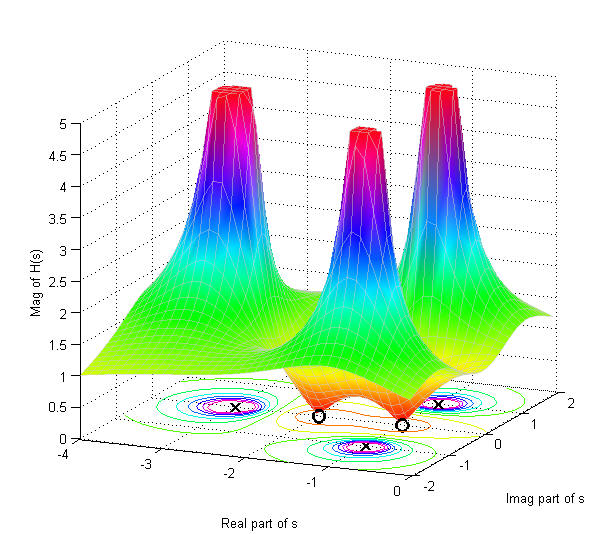
\includegraphics[width=.60\textwidth, height=.50\textwidth]{figs/polezero3d.jpg} } 
\caption{This is the plot of gain $\| \tf(s) \|$ for the transfer function 
\eqref{eq:3pole}, which has 3 poles and 2 zeros (source: \cite{swarth_pole_zero}).  Poles are points $\mu\in\C$ where $| \tf(\mu)| = \infty$.   If our reduced order model has about the same distribution and influence of major (dominant) poles and zeros, then we can say it is a good approximation.  Unfortunately there are no proven results for error bounds with pole/zero matching, but it makes intuitive sense.}
\label{fig:swarth_pole}
\end{figure}





\subsubsection{Transfer function moments}        \label{sec:moments}
\index{transfer function!moments of}

\index{moment matching}
Krylov subspace projection methods boast \emph{moment matching} properties.  The reduced order model transfer function implied by a Krylov subspace method is guaranteed to share a number of  terms of the Taylor series about one or several points, with that of the full unreduced model.  

\smallskip
The transfer function is a rational function, and thus can be represented by a Taylor series about an expansion point $\xp\in\C$, having the general form 
\begin{equation}
                \tf(s) = \sum_{j=0}^\infty (s-\xp )^j \mo{j},  \quad \text{or equivalently,}\quad
  \tf(s+\xp) = \sum_{j=0}^\infty s^j \mo{j}
                \label{eq:tfunc_taylor}
        \end{equation}
        where the Taylor coefficient 
\begin{equation}
\mo{j} =\left. \dfrac{1}{j !}\dfrac{d^j \tf}{d s^j}\right|_{s=\xp}
\label{eq:moment_def}
\end{equation}
is called the $j$-th \emph{moment} of the transfer function about $\xp$.



\paragraph{Moment Matching}
 Suppose the URM (unreduced model) transfer function expressed a a Taylor series about $\xp$ is 
\[
\tf(s) = \mo{0} + (s-\xp)\mo{1} + (s-\xp)^2 \mo{2} + \cdots +(s-\xp)^{n-1} \mo{{n-1}} + \cdots.
\]
A reduced order model (ROM) whose transfer function can be written as 
\[
\tfexp(s) = \moexp{0}  + (s-\xp)\moexp{1} + (s-\xp)^2 \moexp{2} + \cdots +(s-\xp)^{n-1} \moexp{n-1} + \cdots
\]
where 
\[
\moexp{j} = \mo{j} \quad\text{for}\quad j=0,1,2,\cdots,n-1
\]
  is said to \emph{match $n$-moments about $\xp$}.  

Moments can be matched about any number of expansion points; indeed, they are often referred to as \emph{interpolation} points and using several such points is called \emph{rational-interpolation}. 

\subsubsection{Shift-invert representation}
Moment matching properties of Krylov subspace methods are accomplished via the the following reformulation of the transfer function \eqref{eq:tfunc}.

 Let $\xp\in\C$ be a point for which $\xp \E-\A$ is invertible. Then
        \begin{align}
                        \tf(s) &= \CC^T\left(s\E-\A\right)^{-1}\BB\nonumber\\
					&= \CC^T\left(\xp \E - \A + (s-\xp)\E\right)^{-1}\BB\nonumber\\
                                &= \CC^T\left(I-(s-\xp)\H\right)^{-1}\RR 
        \label{eq:tfunc_single_matrix}
        \end{align}
        where
        \begin{equation}
                        \H := (\A - \xp \E)^{-1}\E\quad\textrm{and}\quad \RR := (\xp \E-\A)^{-1}\BB.        
        \label{eq:singlematrixdefs}
        \end{equation}
  \eqref{eq:tfunc_single_matrix} is sometimes called the \emph{shifted} transfer function formulation, with \emph{shift} $\xp$, although it does not depend on $\xp$.  \eqref{eq:tfunc_single_matrix} is the same function regardless of the value of $\xp$ as long as $\A-\xp \E$ is invertible.\footnote{To verify \eqref{eq:tfunc_single_matrix}, note that $I=(\xp \E - \A)^{-1}(\xp \E - \A)$.}  The generally non-sparse $\H = \H(\xp)\in\C^{N\times N}$ is a sort of operator or multiplier, and $\RR=\RR(\xp)\in\C^{N \times \nout}$ is a start-block or start-vector.  $\H=\H(\xp)$ is sometimes called a \emph{shifted-inverse operator}, \emph{shift-and-invert operator}, or \emph{rational operator}, with shift $\xp$.   $\H$ and $\RR$ are the building blocks for the moments of the transfer function about $\xp$.  It should be noted that $\H$ is dense in general and is rarely if ever explicitly formed.  We only need a way to obtain matrix-vector products $\H v$ for vectors $v\in\C^N$. 

The shifted transfer function representation \eqref{eq:tfunc_single_matrix} can alternatively be considered the transfer function for the shifted descriptor system
 \begin{equation}
         \begin{aligned}
                \H \frac{dx}{dt} &= (I - \xp \H) x + \RR u\\
                y &= \CC^T x,
        \end{aligned}
        \label{eq:ds1_shifted}
        \end{equation}   
which is equivalent to \eqref{eq:ds1} for any $\xp$ such that $\A - \xp \E$ is invertible.  This is notable because some order reduction schemes work by replacing $\H$, $\RR$, and and $\CC$ with reduced order approximations $\Himp = V^T \H V$, $\rrimp_n = V^T \RR$, and $\CC_n = V^T \CC$.    We will call such a ROM \emph{implicitly} projected on to $\spn V$, as opposed to the \emph{explicitly} projected model \eqref{eq:ds1_expROM}.   A model obtained via implicit projection is not equivalent to \eqref{eq:ds1_expROM} in general and is undesirable for some applications, but is much cheaper to construct. 

\paragraph{Moment representation}
We now express transfer function moments about $\xp$ in terms of $\H$ and $\RR$. 
        Via Neumann series expansion (power series for matrices) re-write \eqref{eq:tfunc_single_matrix} as
        
\begin{equation}
\begin{aligned}
                \tf(s) &= \CC^T\left(\sum_{j=0}^\infty (s-\xp )^j\H^j\right)\RR \\
			    &= \sum_{j=0}^\infty (s-\xp )^j \CC^T \H^j \RR. 
         \end{aligned}
\label{eq:neumann}
\end{equation}


   The moments $\mo{j}$ from \eqref{eq:tfunc_taylor} are specified exactly in \eqref{eq:neumann}: 
\begin{equation}
\mo{j} = \CC^T \H^j \RR
\label{eq:tfunc_moment}
\end{equation}


Moments \eqref{eq:tfunc_moment} suggest the following moment 
matching method: Compute $n$ terms of the sequence
\begin{equation}
 \RR,\quad \H \RR,\quad \H^2 \RR, \quad\ldots,
\label{eq:power_sequence}
\end{equation}
and then left-multiply the observability constraint $\CC^T$ by each one, giving us $n$ terms of the Taylor series \eqref{eq:neumann}.   The first Krylov subspace projection methods of the early 90s did just that, although moments were not recognized as such at the time.  It was not thought feasible or necessary  to match more than two or three.


\index{moment matching!region of convergence}
\paragraph{Region of convergence for moment matching} The power (Taylor) series representation seems to imply that \eqref{eq:neumann} is only valid for $s$ in a disc of radius $1/\nrm{op}{\H}$ around $\xp$, where the operator norm
\[
 \nrm{op}{\H} =  \sup_{v\neq 0}\left\{  \dfrac{\nrm{}{\H v}}{ \nrm{} {v} } \right\}.
\]
 Then certainly $\nrm{op}{\H} \geq | \lambda_1 |$, where $\lambda_1$ is the largest eigenvalue of $\H$. 
Equivalently,   $\nrm{op}{\H} \geq 1/| (\mu_1-\xp) |$ where $\mu_1$ is the closest pole to $\xp$.   Thus, the 
region of convergence for \eqref{eq:neumann} is the largest disc centered at $\xp$ that does not contain a pole.   The closer $\xp$ is to a pole of the transfer function, the smaller region of convergence we theoretically have for moment matching about $\xp$.
     




\subsubsection{Pad\'e approximation}
\label{sec:pade}\index{pade@\pade{}}
Moment matching is arguably the only reliable means by which we can ensure the quality of a reduced order model, and moment matching techniques have been used at least since the early 70s.  The concept is simple: a reduced model matching more moments about $\xp$ is a more accurate approximation around $\xp$.  Moment matching is obviously only a local quality measure.  We can match moments about several points, thus approximating the transfer function via rational interpolation,  but there is currently no consistent (from model to model) and easily computable  notion of \emph{global} convergence.  

\medskip
How many moments about $\xp$ can we hope to match with a ROM of size (order) $q\ll N$?
\medskip
   
There is, in fact, an upper limit to how many moments a size $n$ ROM can match.   For a SISO model, that is $2q$.   Equivalently, a reduced model that matches $n$ moments must be at least of order $n/2$.  A reduced model with this optimal moment matching property is called a \pade{} model.    \pade{} approximation is historically important in model reduction.  In the past, reduction of LTI systems via transfer function approximation were done with low-order rational approximants, using coefficients listed in so-called Routh and \pade{} tables \cite{shamash1974padetype, shamash1975model}.   

\begin{itemize}
\item For a SISO model the transfer function \eqref{eq:tfunc} is a scalar-valued proper rational function over $\C$.   which suggests the  \textbf{\pade{} approximant} \emph{about $\xp$, of order $(p,q)$},
\begin{align}
\tf_{p,q}(s+\xp) =  \frac{b_0 + b_1 s + b_2 s^2 +  \cdots + b_ps^p}%
		{1 + a_1 s + a_2 s^2 + \cdots + a_q s^q},
\label{eq:pade_approximant}
\end{align}
 with  $p < q$.\footnote{note that $\tf(s+\xp)=\frac{P(s)}{Q(s)}$ is equivalent to $\tf(s)=\frac{P(s-\xp)}{Q(s-\xp)}$.  We use the former for simpler notation.} Note that $a_0=1$, so that a \pade{} representation of order $(p,q)$ has $p+q+1$ parameters.  

MIMO model transfer functions have an analogous \emph{Matrix \pade{}} representation. 
\end{itemize}

\smallskip
For a LTI (linear) SISO system model of order $N$, the transfer function is in fact a quotient of two polynomials and can be represented \emph{exactly} by \eqref{eq:pade_approximant}, with appropriate $p< q\leq N$.     The convention in model reduction via \pade{} approximation is to assume that $p=q-1$ in  \eqref{eq:pade_approximant}, and refer to the \pade{} approximant $\tf_{q-1,q}$ with $2q$ parameters, as $\tf_q$.    The \pade{} model of order $q$ is an optimal $2q$-parameter model and we cannot do better with $2q$ coefficients.

Consider the following equivalent representations of the transfer function  \eqref{eq:tfunc}: The order-$q$ \pade{} approximant
\begin{align}
\tf_q(s+\xp) &=  \frac{b_0 + b_1 s + b_2 s^2 +  \cdots + b_ps^{q-1}}%
		{1 + a_1 s + a_2 s^2 + \cdots + a_q s^q}\label{eq:tf_pade}\\
	&= x_\infty + \sum_{j=1}^{q^\prime} \frac{x_j}{s-\mu_j}\qquad q^\prime\leq q
\label{eq:tf_pole_residue}
\end{align} 
with $q \leq N$, and the Taylor series expansion 
\begin{equation}
\tf(s+\xp) = \sum_{j=0}^\infty \mo{j} s^j, 
\label{eq:tf_moments}
\end{equation}
both approximations centered at $\xp$.
\eqref{eq:tf_pade} is a restatement of  \eqref{eq:pade_approximant} with $p=q-1$.  \eqref{eq:tf_pole_residue} is the partial fraction decomposition of \eqref{eq:tf_pade} and is called the \emph{pole-residue} formulation of the transfer function.  There are $q^\prime\leq q$  finite poles $\mu_j\in\C$ of the transfer function, and the $x_j$ are the associated residues.   The constant term $x_\infty$ is the residue associated with poles at $\infty$, which we will address later.  
 
\pade{} approximation and moment matching are related by equating \eqref{eq:tf_pade},\eqref{eq:tf_pole_residue} with \eqref{eq:tf_moments}.     A \pade{} model of order $q$ is theoretically constructed by setting 
\[
 \sum_{j=0}^{2q-1} \mo{j} s^j  =
  \frac{b_0 + b_1 s + b_2 s^2 +  \cdots + b_ps^{q-1}}%
	{1 + a_1 s + a_2 s^2 + \cdots + a_q s^q}
\]
and solving a $q \times q$ system for coefficients $a_j$ of the denominator polynomial of \eqref{eq:tf_pole_residue}, given  that moments $\mo{j}$ about $\xp$ are given by $\mo{j} = \CC^T \H^j \Rr$.

Constructing an order-$q$ \pade{} model from $2q$ explicitly computed moments   $\mo{j} = \CC^T \H^j \Rr$ is a viable model-reduction method in exact arithmetic, but it involves a badly-conditioned solve and the iterates $\H^j \Rr$  converge to an eigenvector of $\H$ as $j>0$ increases.  It is not practical for $j>10$, however it was at one time a popular model reduction method called AWE, which has since given way to iterative subspace methods, such as those exploiting the Krylov iteration.  The underlying moment matching property is still the appeal of these methods, which are considered \pade{} or \emph{\pade{}-type} methods and considered to be descendants of AWE.  A \pade{}-type method is one that employs a moment matching strategy, allthough the reduced model of a given size is not optimal in the number of moments matched.  Most contemporary moment matching methods produce \pade{}-type models, mostly because true \pade{} reduced models are not guaranteed to be stable, even if the original model is stable. 


The analog to \pade{} for for a general MIMO model is called matrix-\pade{}, and since moments are $\nout \times \nin$ matrices we have a different bound for the number of moments matched by a matrix-\pade{} model.

 The approximation $\tfexp_n(s)$ of size $n$ that satisfies
        \begin{align}
                \tf(s) &= \tfexp_n(s) + \bigO{(s-\xp )^{q(n)}}
                \label{eq:pade}
        \end{align}
        is called a  \emph{Pad\'{e}  approximation} if the number of matched-moments $q(n)$ is as large as possible. Otherwise, if any moments are matched we 
        call it a Pad\'{e}-type approximation.  It was shown by \cite{AN} that 
\begin{equation}
	q(n) \leq \bigg\lfloor \frac{n}{\nin} \bigg\rfloor + \bigg\lfloor \frac{n}{\nout} \bigg\rfloor,
\label{eq:pade_bound}
\end{equation}
where $\nin$ is the number of inputs and $\nout$ is the number of outputs of the system.  This is because the moments are $\nout \times \nin$ blocks.  Since each moment 
\[
\mo{j} = \CC^T \H^j \RR
\]
is a  $\nout \times \nin$ (possibly complex-valued) block, each further moment matched requires a possibly large increase in the size of the reduced model.  In the $\nin=\nout=1$ (SISO) case the  Pad\'{e}  (optimal) approximation exhibits $q(n)= 2n$, or $2n$ moments matched for an approximate model of dimension $n$.    
        Although it is possible to produce a Pad\'{e}
        approximation of the transfer function, we know from \cite{AN} 
        that such a model in general does not preserve stability or passivity.  
        For a more reliable approximation we expect $q(n)=n$; a SISO model of size $n$ (determined by $n$-iterations about $\xp$) matches $n$ moments about $\xp$.

The definition of a \pade{} model about an expansion point $\xp$ extends to multiple points and is discussed in \cite{multipoint_pade}.


\paragraph{Asymptotic Waveform Evaluation (AWE)}
This is a brief description of the AWE  method of \cite{AWE}, which has historical and computational significance in that it exemplifies \emph{explicit moment matching}.  The moments $\mo{j}(\xp) = \CC^T \H^j \Rr$ about $\xp$ are explicitly computed.   In contrast, modern methods often produce models with moment matching properties, but moments of the model are never actually computed. AWE was one of the early attempts at matching more than one or two moments of a system transfer function.  It is also a good example of how mathematically equivalent methods can be very different when implemented on a computer.   AWE and the later PVL (\pade{} via Lanczos), which is a Krylov subspace projection method, in theory both produce a \pade{} model by matching transfer function moments about $\xp$, so they are mathematically equivalent.

The SISO transfer function has the \pade{} form 
\begin{equation}
\tf_{q}(s) = \frac{P(s)}{Q(s)}
\label{eq:tfunc_pade}
\end{equation}
where
\[
P(s) = \sum_{j=0}^{q-1} (s-\xp)^j b_j \qquad \text{and}\qquad
Q(s) =\sum_{j=0}^{q} (s-\xp)^j a_j.
\]
Then 
\[
\underbrace{\left( \sum_{j=0}^{q-1} (s-\xp)^j b_j  \right)}_{P(s)}
=
\underbrace{\left( \sum_{j=0}^{2q-1} (s-\xp)^j \mo{j} \right)}_{\tfexp_q(s)}
\underbrace{\left( \sum_{j=0}^{q} (s-\xp)^j a_j \right)}_{Q(s)},
\] 
which suggests we solve the  system 
\begin{equation}
\mat{\mo{0} & \mo{1} & \cdots & \mo{q-1}  \\
       \mo{1} & \mo{2} & \cdots & \mo{q}  \\ 
\vdots & \vdots & \ddots & \vdots \\
\mo{q-1} & \mo{q} & \cdots & \mo{2q-1} 
}
\mat{a_q \\ a_{q-1} \\ \vdots \\ a_1} =
\mat{\mo{q} \\ \mo{q+1}\\ \vdots \\ \mo{2q-2}}
\label{eq:AWE_system}
\end{equation}
to determine the coeffcients  $a_j$ of the characteristic polynomial $Q(s)$.
 
 Recall that we can compute transfer function moments 
\begin{equation}
\mo{j} = \CC^T \H^j \Rr.
\tag{\ref{eq:tfunc_moment}}
\end{equation}

\begin{description}
\item{\bf AWE  method for SISO model reduction:}\cite{AWE} \\
AWE constructs an order-$q$ \pade{} approximant about $\xp$
\begin{align}
\tf_q(s+\xp) &=  \frac{b_0 + b_1 s + b_2 s^2 +  \cdots + b_ps^{q-1}}%
		{1 + a_1 s + a_2 s^2 + \cdots + a_q s^q}\tag{\ref{eq:tf_pade}}\\
	&= x_\infty + \sum_{j=1}^{q^\prime} \frac{x_j}{s-\mu_j}, \qquad q^\prime\leq q
\tag{\ref{eq:tf_pole_residue}}
\end{align} 
 of the transfer function \eqref{eq:tfunc}, from $2q$ moments of the original model.  

Given $\H$ and $\Rr$ as defined in 
\eqref{eq:singlematrixdefs}, we compute $2q-1$ terms of the sequence
\begin{equation}
 \Rr, \H \Rr,  \H^2 \Rr, \ldots, \H^{2q-1} \Rr,
\label{eq:krylov_terms}
\end{equation}
and left multiply $\CC^T$ to obtain $2q$ system moments $\mo{j} = \CC^T \H^j \Rr$, for $j=0,2,...,2q-1$.  We then solve  \eqref{eq:AWE_system} for coefficients $a_j$ of the denominator polynomial 
\[
1 + a_1 s + a_2 s^2 + \cdots + a_q s^q 
    \quad =  \quad (s-\mu_1)(s-\mu_2)\cdots (s-\mu_q),
\]   
and compute its roots $\mu_j$, which are poles of the transfer function.  We then solve another order-$q$ system of equations for residues $x_j$ and $x_\infty$,  thus yielding the pole-residue form \eqref{eq:tf_pole_residue}. 
\end{description}

\medskip
 AWE suffers from numerical trouble resulting from the fact that the power sequence \eqref{eq:power_sequence} converges to an eigenvector of $\H$.  
  The terms of the sequence quickly become linearly dependent so the systems to be solved (e.g. \eqref{eq:AWE_system}) are badly conditioned.    Thus, AWE is not practical for $n>10$ or so.    However, moment matching is one of the few ways  to gage the quality of a reduced model , and although we will not explicitly compute transfer function moments,  we try to develop methods with moment matching properties.   The convergence of the sequence \eqref{eq:krylov_terms} to an eigenvector is the basis of the Power Iteration, addressed in \S\ref{sec:iterations}.




\subsubsection{Invariant subspaces}\label{sec:invariant_subspaces}
We first introduce the notion of an invariant subspace under an operator and extend it to that of a general matrix pencil.
 
\index{invariant subspace}
Given a transformation $\H:\C^N \rightarrow \C^N$, a subspace $\Q$ of $\C^N$ is called $\H$-invariant or \emph{invariant under}, or \emph{invariant with respect to} $\H$ if 
\begin{equation}
\H\Q \subseteq \Q.
\label{eq:op_invariance}
\end{equation}

The span of a set of eigenvectors of $\H$ is an ($\H$-)invariant subspace, and an invariant subspace always has a basis consisting of eigenvectors of $\H$.   

If $Q$ is a basis for $\Q$ then
\begin{equation}
\H Q = Q T
\label{eq:similarity}
\end{equation}
for some matrix $T\in\C^{\ell\times\ell}$.  If the basis vectors are eigenvectors $Z$ then \eqref{eq:similarity} becomes
\[
\H Z = \Lambda Z,
\] 
where $\Lambda = \text{diag} \{ \lambda_1, \lambda_2, ...,\lambda_\ell \}$ is a diagonal matrix of eigenvectors associated with the vectors
 $Z = \mat{z_1 & z_2 & \cdots & z_\ell}$. 
\index{Schur vectors}

If the basis $Q=\mat{u_1 & u_2 & \cdots & u_\ell}$ for the $\H$-invariant subspace 
\[
\Q = \spn \mat{u_1 & u_2 & \cdots & u_\ell}=\spn \mat{z_1 & z_2 & \cdots & z_\ell}
\] 
is orthonormal then we call vectors $u_j$ \emph{Schur-vectors} and sometimes call $\Q$ a Schur space.   Also, \eqref{eq:similarity} is called a \emph{Schur-decomposition}, and $T$ is upper triangular with eigenvalues $\lambda_j$ associated with $z_j$ along its diagonal.   A Schur decomposition is often preferred over an eigen-decomposition because it is easier to compute and Schur vectors are more numerically stable. 



\medskip
Now we extend the notion of invariance to the linear matrix pencil $\A-s\E$.   A \emph{matrix pencil} \index{matrix pencil} is a polynomial
\[
\sum s^j M_j
\]
 over $s\in\C$ with matrix coefficients $M_j\in\C^{N\times N}$.  The \emph{linear matrix pencil} $(\A- s \E)$  is generally denoted as $(\A,\E)$. 


 An eigenvalue \index{eigenvalue, eigenvector (generalized)} of  matrix pencil $(\A,\E)$, called  a \emph{generalized} eigenvalue, is a $\mu\in\C$ such that $(\A-\mu \E)z=0$ has nonzero solutions $z\neq 0\in\C^N$, which are called eigenvectors.

An eigenvalue $\mu$ of $(\A,\E)$ has two associated eigenvectors: a left vector $w$ and a right vector $z$, both in $\C^N$, such that
\[
\A z = \mu \E z
\]
and
\[
\c{w}\A =\mu \c{w}\E, \quad\text{or equivalently } \c{\A}w =\mu \c{\E} w,    
\]
where $\c{(\cdot)}$ denotes the hermitian-conjugate transpose.  It is common in linear algebra to speak of  an eigen-\emph{pair} $(\mu,z)$, or an eigen-triplet  $(\mu,w,z)$. 


A collection of $\ell$ right-eigenvectors as columns of $Z =\mat{z_1&z_2&\cdots&z_\ell}$  has the property that
\begin{equation}
\A Z= \E Z \M,
\label{eq:right_eigen}
\end{equation}
 where $\M = \text{diag}\mat{\mu_1 & \mu_2 &\cdots&\mu_\ell}$ is a diagonal matrix of the associated eigenvalues.  $Z$ is a basis for a subspace of the \emph{right-eigenspace} of $(\A,\E)$.

\bigskip
The notion of invariance under a general operator $\H$ extends to that of a matrix pencil. The subspace $\Q = \spn Z$ is  called invariant or \emph{deflating} \cite{stewart1972sensitivity} with respect to $(\A,\E)$ if
\begin{equation}
\dim \left(\A \Q + \E \Q  \right) \leq \dim \Q.
\label{eq:generalized_invariance1}
\end{equation}
 For a regular matrix pencil $(\A,\E)$ and any $\xp\in\C$ that is not an eigenvalue of $(\A,\E)$ it is shown in \cite{gracia1995stability} that $(\A,\E)$-invariance is equivalent to $\H$-invariance for 
\begin{equation}
\H = (\A-\xp \E)^{-1} \E, 
\label{eq:AE}
\end{equation}
which happens to be the shift-invert operator defined by \eqref{eq:singlematrixdefs}.   

\smallskip
Then $\H(\xp)=(\A-\xp \E)^{-1} \E$ has the same eigenvectors (regardless of $\xp$) as the pencil $(\A,\E)$.   An eigenvalue $\lambda$ of $\H$ and its corresponding eigenvalue $\mu$ of $(\A,\E)$ are related by   
\begin{equation}
      \lambda = \frac{1}{\mu-\xp}, \qquad \mu = \xp + \frac{1}{\lambda}
	\label{eq:pole_eig}
\end{equation}
and they share the same eigenvector. That is, 
\[
\begin{aligned}
\H z &= \lambda z \\
&= \left( \frac{1}{\mu-\xp} \right) z
\end{aligned}
 \quad \Longleftrightarrow \quad 
\begin{aligned}
\A z &= \mu \E z \\
&= \left(\xp + \frac{1}{\lambda}\right)\E z
\end{aligned} 	
\]
To see this, observe that 
\begin{equation}
\begin{aligned}
(\mu \E - \A) &= \left[ (\mu-\xp)\E + (\xp \E-\A)                     \right]  \\
&= [ (\mu-\xp)\underbrace{(\xp \E-\A)^{-1}\E}_{-\H} + I ]  \\
&= \left[ (\mu-\xp)\H - I                                \right]  \\
&= \left[ \H-\left(\frac{1}{\mu-\xp}\right)I             \right]  \\
&= ( \H-\lambda I  ) .
\end{aligned}
\label{eq:shift_invariance}
\end{equation}
In other words, invariant subspaces under the shifted operator $\H(\xp)$ are shift-invariant.  This is useful because if we decide to change the shift $\xp$, any previously discovered invariant subspace will be still be invariant under the new operator.

\subsubsection{Pole-Residue representation}
Recall the transfer function  
\begin{equation}
\tf(s) = \CC^T\left(s\E-\A\right)^{-1}\BB,\tag{\ref{eq:tfunc}}
\end{equation}
which prominently features the linear matrix pencil $(\A,\E)$.  


\smallskip
\noindent The $\A$ and $\E$ that arise from Modified Nodal Analysis \cite{MNA} circuit representations are singular in general.  In particular, $\E$ is singular, which means $(\A,\E)$ has eigenvalues at $\infty$ at least some of which are associated with the null space of  $\E$.  

\paragraph{Poles/residues from standard transfer function formulation}
Let us assume that $(\A,\E)$ has a full eigen-decomposition 
        \begin{equation*}
                \A Z = \E Z \M \quad \text{and}\quad \A^T W = \E^T W \M 
        \label{eq:genEigDecomp}
        \end{equation*}
        where $Z,W\in\C^{N\times N}$ represent the
        right and left eigenspaces of $(\A,\E)$, respectively, and $\M$ is the diagonal matrix of eigenvalues $\mu_j\in\C \cup \{\infty\}$.  Note that since $\A$ and $\E$ are real, every eigenvalue is real, infinite,  or is one of a complex conjugate pair.
   
The left and right eigenvectors are orthogonal, and can be scaled\footnote{This scaling is not generally the default for eigensolver algorithms.}  so that $\c{W} \E Z = I$. Then 

\begin{equation}
\begin{aligned}
\tf(s) &= \CC^T(s\E-\A)^{-1}\BB\\
 &= \CC^T ( W^{-H} (sI-\M) Z^{-1} )^{-1}\BB \\
 &= \CC^T Z (sI-\M)^{-1} \c{W} \BB \\
 &= \CC^T Z \left(\sum_{j=1}^\npol \dfrac{1}{s-\mu_j} \right) \c{W} \BB.\\
\end{aligned}
\label{eq:tfunc_eigen}
\end{equation}
The pole (eigen) decomposition \eqref{eq:tfunc_eigen}  of the transfer function suggests that it can be approximated if we have some eigen information about $(\A,\E)$; poles $\mu_j\in\C$ located nearest to the segment $S\in i\R^+$ as illustrated in  figure~\ref{fig:ex1b_tfunc}, because they cause $1/(s-\mu_j)$ to be large.   

\bigskip 
For the sake of expressing \eqref{eq:tfunc_eigen} without clutter we assumed all eigenvalues are simple and finite.  Actually, multiple eigenvalues are possible and eigevalues at infinity are inevitable because $\E$ is singular.  The eigenspace associated with infinite eigenvalues is the nullspace of $\E$. 

Recall the left and right hand sides $\CC^T Z\in \C^{\nout \times N}$ and $\c{W} \BB\in \C^{N\times \nin}$ from \eqref{eq:tfunc_eigen} and consider the partitions 
\[
\CC^T Z = \mat{\hat{c}_1 & \hat{c}_2 &\cdots&\hat{c}_N}
\]
and 
\[
\BB^T W = \mat{\hat{b}_1 & \hat{b}_2 &\cdots&\hat{b}_N}
\]
into $N$ columns.

Then we can express the the pole-residue form of transfer function \eqref{eq:tfunc} as 
\begin{equation}
          \tf(s)  =  \sum_{\mu_j=\infty} \hat{c}_j \hat{b}_j^T +
			   \sum_{\mu_j\neq\infty} \frac{\hat{c}_j \hat{b}_j^T}{s-\mu_j}\label{eq:comp_pole_sum}.
\end{equation}
Note that $\hat{c}_j$ and $\hat{b}_j$ are scalars if this is a SISO model. Generally, $\hat{c}_j \hat{b}_j^T\in\C^{\nout \times \nin}$.  The transpose $\hat{b}_j^T$ is in fact a transpose and not a conjugate-transpose, even if $\hat{b}_j$ is complex-valued.  
 

\smallskip
 Our necessary assumption  $\c{W} \E Z = I$ is not the default scaling for eigensolvers in practice.  In that case, we must consider the scaling factor
\[
\xi_j = 1 / w_j^H \E z_j
\]
for $j=1,2,\ldots,q$ and \eqref{eq:comp_pole_sum} generalizes to 
\begin{equation}
          \tf(s)  =  \sum_{\mu_j=\infty} \xi_j\hat{c}_j \hat{b}_j^T +
			   \sum_{\mu_j\neq\infty} \xi_j\frac{\hat{c}_j \hat{b}_j^T}{s-\mu_j}\label{eq:comp_pole_sum_gen}.
\end{equation}

\paragraph{Poles and residues from shifted formulation}\label{sec:polewts_shifted}
For model reduction it is often favorable to work with the so-called $\xp$-shifted transfer function 
\[
\tf(s) = \CC^T \left(I - (s-\xp)\H \right)^{-1} \RR \tag{\ref{eq:tfunc_single_matrix}},
\] 
rather than the standard formulation \eqref{eq:tfunc}.  For that we derive a sum that is term-by-term equivalent to  \eqref{eq:tfunc_eigen} and \eqref{eq:comp_pole_sum} but involves the eigen-decomposition of $\H$, rather than $(\A,\E)$.   

 Assume that $\H$ is diagonalizable with right-eigenbasis $Z$, so that    
\[
\H Z =  Z \Lambda 
\] 
for a $N\times N$ diagonal matrix $\Lambda=\mat{\lambda_1, \lambda_2,\ldots,\lambda_N}$ of eigenvalues.

Then
\begin{align}
\tf(s) &= \CC^T (I - (s-\xp)\H )^{-1} \RR\nonumber\\
&= \CC^T \left( Z (I - (s-\xp)\Lambda )Z^{-1} \right)^{-1} \RR \nonumber\\
&= (\CC^T Z) \Delta(s) (Z^{-1}\RR)
\end{align}
where $\Delta(s)=\left( I - (s-\xp)\Lambda \right)^{-1}$ is a diagonal matrix with diagonal entries $\delta_{j}(s) =1-(s-\xp)\lambda_j$, or equivalently
\begin{equation}
\delta_{j}(s) =
\begin{cases}
\dfrac{\xp-\mu_j}{s-\mu_j},   & \mu_j \neq \infty\\
1, & \mu_j = \infty. 
\end{cases}
\label{eq:delta_def}
\end{equation}

Then for 
\[
\CC^T Z = \mat{\hat{f}_1 & \hat{f}_2 &\cdots&\hat{f}_N} \quad\text{and}\quad
(Z^{-1}\RR)^T = \mat{\hat{g}_1 & \hat{g}_2 &\cdots&\hat{g}_N},
\]
we have
\begin{align}
\tf(s) &= \sum_j \frac{\hat{f}_j\hat{g}_j^T}{1-(s-\xp)\lambda_j} \label{eq:comp_eig_sum}\\
&= \sum_{\lambda_j=0} \hat{f}_j\hat{g}_j^T + \sum_{\lambda_j \neq 0} \frac{\xp-\mu_j}{s-\mu_j}\hat{f}_j\hat{g}_j^T\nonumber\\
&= \sum_j \delta_j(s) \hat{f}_j \hat{g}_j^T,\label{eq:comp_pole_alt} 
\end{align}
where $\delta_j(s)$ is from \eqref{eq:delta_def}. The transpose $\hat{g}_j^T$ is in fact a non-conjugate transpose, even if $\hat{g}_j$ is complex-valued.   Both  $\hat{f}_j$ and $\hat{g}_j^T$ are scalars in the SISO case.
Note that a zero eiqenvalue $\lambda_j=0$ of $\H$ corresponds to an infinite $\mu_j=\infty$ pole (eigenvalue of $(\A,\E)$). 


\subsubsection{Pole weight}\label{sec:pole_dominance}
\index{dominant pole}
Recall that poles of the transfer function $\tf(s) = \CC^T\left(s\E-\A\right)^{-1}\BB$ are values $\mu\in\C \cup \infty$ such that $\|\tf(\mu)\|=\infty$. Poles of $\tf(s)$ are eigenvalues of the matrix pencil $(\A,\E)$, but their significance is determined by $\BB$ and $\CC$. Pole dominance is a measure of a pole's influence on the transfer function frequency response $\tf(i \omega)$ on an interval of the $\Im$-axis (or all of it).   
\index{mass!system}\index{mass!pole}
Pole-residue formulations  \eqref{eq:comp_pole_sum_gen} and \eqref{eq:comp_pole_alt} suggest a hierarchy of poles' importance for approximation, often called pole-dominance \cite{Aguirre}.  

 We will define a measure of pole-dominance, which we will call its \emph{mass} or \emph{weight} with respect to the frequency response domain $i[\omega_1,\omega_2]\subset\C$.  It is similar to the modal dominance index (MDI) of \cite{Aguirre}, but it considers a pole's influence over the frequency response domain rather than all of the positive $\Im$-axis. 

 From \eqref{eq:comp_pole_alt}, over the interval $i[\omega_1,\omega_2]$ of interest on the $\Im$-axis we have 
\begin{equation}
\nrm{\infty}{\tf(i\omega)} \leq  \sum_j \nrm{\infty}{\delta_j(i\omega)} \|\hat{f}_j\|_1 \nrm{1}{\hat{g}_j},
\label{eq:system_mass}
\end{equation}
which is a sum of positive numbers, each one associated with a pole $\mu_j$.  Then a relatively large pole-weight, or \emph{pole-mass} 
\begin{equation}
\gamma_j =  \nrm{\infty}{\delta_j(i\omega)} \|\hat{f}_j\|_1 \nrm{1}{\hat{g}_j}
\label{eq:pole_weight}
\end{equation}
from \eqref{eq:system_mass}  indicates that $\mu_j$ is a dominant pole.   

For a SISO model, $\hat{f}_j$ is a scalar so $\|\hat{f}_j\|_1=|\hat{f}_j|$ and it represents the weighting of the pole $\mu_j$ by the left-hand multiplier $\CC=\Cc$ of the transfer function \eqref{eq:tfunc}.   

A MIMO system has $\nout$ such left-multipliers in the form of $\CC=\mat{\Cc_1 & \Cc_2 &\cdots&\Cc_\nout}$ and each one has an associated element in the column vector $\hat{f}_j=(\hat{f}_{1j},\hat{f}_{2j},\dots,\hat{f}_{\nout j}) \in\C^\nout$.  By summing them we get an overall sense of how much $\mu_j$ is favored by $\CC$.   Thus we use the $1$-norm (column-sum)  
\[
\|\hat{f}_j\|_1 = \sum_i |\hat{f}_{ij}|.
\]

 The reasoning for using $\nrm{1}{\hat{g}_j}$ in \eqref{eq:system_mass} is similar.  

The scalar-valued function $\delta_j(i\omega)$ represents the influence of pole $\mu_j$ on the system frequency response via its proximity to the segment $i[\omega_1,\omega_2]$ of interest, and we take its maximum value 
\begin{align}
\nrm{\infty}{\delta_j(i\omega)} &= \max_{\omega\in [\omega_1,\omega_2]}| \delta_j(i\omega)|\nonumber\\
&= \begin{cases}
\dfrac{| \xp-\mu_j|}{\min\{|\mu_j-\omega_1|,|\mu_j -\omega_2|,|\Re(\mu_j)|  \}},   & \mu_j \neq \infty\\
1, & \mu_j = \infty
\end{cases}
\label{eq:pole_wt_delta}
\end{align}
over that interval.
The value $\min\{|\mu_j-\omega_1|,|\mu_j -\omega_2|,|\Re(\mu_j)|  \}$ is merely the distance of $\mu_j$ to the segment $i[\omega_1,\omega_2]$, as illustrated in figure~\ref{fig:MDI_examp}.  Conjugate pairs must be considered together, so when determining weight we actually consider $\Re(\mu_j)+ i|\Im(\mu_j) |$, rather than $\mu_j$. That way, each member of the pair gets assigned the same weight.

\paragraph{Total system-mass}
The right-hand-side of \eqref{eq:system_mass} (i.e. $\sum_j \gamma_j$),
 is the total mass of the system \eqref{eq:ds1} with respect to $ i[\omega_1,\omega_2]$, and can be used as a measure of ROM convergence.  The combined weight of a few dominant poles often comprises most of a system's total mass.

\begin{figure}
\centering
\putfig{.8}{MDI_examp.png}
\caption{\label{fig:MDI_examp} The red (solid) segment on the $\Im$-axis is the segment $i(\omega_0, \omega_1)$ of interest.  In this case it looks like it extends to the origin but it does not.  The arrows indicate how we define a pole's distance to the segment, which we use to determine the pole's weight. Conjugate pairs must be considered together, so when determining weight we always consider $\Re(\mu)+ i|\Im(\mu) |$, rather than $\mu$. That way, each member of the pair gets assigned the same weight.}
\end{figure}







\begin{figure}[htb]
\centering
\putfig{.48}{fr308s_1.png}\hfill
\putfig{.48}{fr308s_2.png}
\caption{\label{fig:30812tfuncs}Frequency response gain plots for \texttt{ex308s11} and \texttt{ex308s22}, two SISO components of a single MIMO system.   They  share the same system pencil $(\A,\E)$ and thus the same system eigenvalues.  They differ in controllability and observability condition vector pairs:  $(\Bb_1,\Cc_1)$ and $(\Bb_2,\Cc_2)$, respectively.  Both systems have the same poles, but weighted differently by $\Bb_j$ and $\Cc_j$, giving two rather different frequency responses.  The respective surface plots of $\tf(s)$ below, with frequency response gain (over the $\Im-$axis) highlighted, show that the influence of poles and zeros is fairly uniform in the first example, and in the second we see a clear distinction between heavy and light poles. }
\label{fig:examps308s12}
\putfig{.48}{308s_1_full.png}\hfill
\putfig{.48}{308s_2_full.png}
\end{figure}

\begin{figure}[htb]
\centering
\putfig{.48}{308s_2pwt.png}
\caption{Pole weight order-of-magnitude distribution for \texttt{ex308s11} and \texttt{ex308s22}.  In the second example, there is a clear separation between almost insignificant poles, and poles of nearly uniform influence.  In the first example there is one dis-proportionally dominant pole (located at the origin) and the rest vary.  Plots of the poles are below.  Note that the locations the of poles are all the same, only their weights vary.  Several appear to be on the $\Im$-axis, but they are only close, meaning within $10^7$ of the axis in this scaling.}
\putfig{.48}{308s_2dpoles.png} 
\end{figure}



\begin{figure}[htb]
\centering
\putfig{.70}{fr308s_3.png}

\putfig{.45}{308s_3dpoles.png}\hfill
\putfig{.45}{308s_3pwt.png} 
\medskip

\putfig{.48}{308s_3_full1.png}\hfill
\putfig{.48}{308s_3_full2.png} 
\caption{Here are similar plots for a third SISO model \texttt{ex308s12} from the same family as those in figure~\ref{fig:examps308s12}.  The three \texttt{ex308} SISO models \texttt{s11}, \texttt{s22}, and \texttt{s12} are from one MIMO circuit model with $\BB=\CC\in\R^{308 \times 2}$ ($\nin=2$ inputs, $\nout=2$ outputs).   This example is more like \texttt{s11} than \texttt{s22} in that the pole weights are relatively uniform.  In \texttt{s12}, more poles are dominant.}
\end{figure}
\clearpage




\subsubsection{ROM transfer function via projection }\label{sec:projected_ROMs}
The URM (unreduced model) transfer function formulations \eqref{eq:tfunc} and \eqref{eq:tfunc_single_matrix} exist only in theory for large applications, which can be on the order of $10^9$ at the time of this writing.    \eqref{eq:tfunc} and \eqref{eq:tfunc_single_matrix} are mathematically equivalent.  Subspace projected ROM transfer functions can be obtained via \emph{explicit} projection, or \emph{implicit} projection, yielding two forms similar to \eqref{eq:tfunc} and \eqref{eq:tfunc_single_matrix} that are \emph{not} mathematically equivalent but they converge to the  URM (unreduced) transfer function \eqref{eq:tfunc}, \eqref{eq:tfunc_single_matrix} as the projection subspace approaches $\C^N$.

\medskip
Let $V\in\C^{N \times n}$ be a matrix with orthogonal columns that form a basis of our projection subspace $\K$.  
If we make the orthogonal projections 
\begin{equation*}
          \A_n := V^T \A V, \quad \E_n := V^T \E V, \quad \CC_n := V^T\CC, \quad \BB_n := V^T\BB,
          \tag{\ref{eq:exp_projections}}
 \end{equation*}	
of realization $(\A,\E,\BB,\CC)$ on to $\K$,\footnote{assuming the matrix pencil $(\A_n,\E_n)$ is regular} the {\bf explicitly projected} \index{transfer function!projected!explicitly}\index{explicit projection (ROM)} model $(\A_n,\E_n,\BB_n,\CC_n)$ has transfer function    
         \begin{equation}
                        \tfexp_n(s) = \CC_n^T\left(s\E_n-\A_n\right)^{-1}\BB_n.
         \label{eq:rm_explicit}
         \end{equation}
The explicitly projected model  has the nice property  that the projected ROM \eqref{eq:rm_explicit} of a stable system is stable if the projection basis $V$ is real-valued.  No poles of the ROM transfer function have positive real part, with the possible  exception of remote approximations to poles of \eqref{eq:tfunc} at $\infty$, and even this can most-likely be attributed to numerical error.  The classic explicit projection ROM method is PRIMA, given by \cite{PRIMA}.  In that case, the subspace for projection is a  Krylov subspace and the ROM is shown to be of Pad\'e-type, matching $n$ moments with a model of dimension $n$.   

More generally we may construct a pair of bi-orthogonal bases $V$ and $W$ (with $V^TW=I$),  and explicitly make the oblique projections 
\[
\A_n := V^T \A W, \quad \E_n := V^T \E W, \quad \CC_n := \c{W}\CC, \quad \BB_n := V^T\BB.
\]
Most projected methods do have one and two-basis variants; they are  respectively called \emph{orthogonal} and \emph{oblique} projection methods.

\bigskip
Some iterative subspace methods, notably Krylov subspace methods,  use the operator $\H=\H(\xp)$ simultaneously construct  bases $V $and $W$ \emph{and} a projected operator matrix $\Himp\in \C^{n \times n}$, where
\[
\Himp = V^T \H W.
\]
This permits what we will call the \textbf{implicitly projected} ROM transfer function 
\index{transfer function!projected!implicitly}\index{implicit projection (ROM)}
 \begin{align}
      \tfimp_n(s) &=  \c{\CC_n} \left(I-(s-\xp )\Himp\right)^{-1}\rrimp_n,
      \label{eq:rm_implicit}
      \end{align}
      where
      \[
        \CC_n := \c{W} \CC \quad\textrm{and}\quad \rrimp_n := V^T \RR.
      \]
Clearly this is the projected ROM analog to the ``shifted'' transfer function \eqref{eq:tfunc_single_matrix}.
The implicitly projected type of MOR transfer function was made popular by \cite{PVL} (and independently by \cite{gallivan1994asymptotic}) where it was shown that such a ROM is Pad\'e, hence \emph{Pad\'e Via Lanczos}.   The insight of \cite{PVL,gallivan1994asymptotic} to apply a projected process for moment matching was provided by \cite{gragg1974matrix} in 1974.  PVL and its predecessor AWE are mathematically equivalent but the Krylov subspace projected variant PVL works much better in practice.  Instead of models matching a handful of moments, any number of moments can be matched by PVL, or all of them.  A variant of PVL using the one-sided Arnoldi process and using one orthogonal basis $V=W$ to make \eqref{eq:rm_implicit} was shown to preserve passivity for RCL circuit models by \cite{arnoldiMOR}.  
  
We call \eqref{eq:rm_implicit} the transfer function for the implicitly projected model because it exists without a projected realization $(\A_n,\E_n,\BB_n,\CC_n)$ from \eqref{eq:exp_projections}.   The reduced model implied by \eqref{eq:rm_implicit} is actually
  \begin{equation}
         \begin{aligned}
                \Himp \frac{d\tilde{x}}{dt} &=  (I+\xp \Himp)\tilde{x} + \rrimp_n u\\
                \hat{y} &= \CC_n^T \tilde{x},
        \end{aligned}
        \label{eq:implied_ds1}
        \end{equation}
which is not equivalent to the explicitly projected system 
 \begin{equation}
         \begin{aligned}
                \E_n \frac{dz}{dt} &= \A_nz + \BB_n u\\
                \hat{y} &= \CC_n^T z,
        \end{aligned}
        \tag{\ref{eq:ds1_expROM}}
        \end{equation}
 given the same basis $V$, unless $V$ spans $\C^N$ (i.e. $n=N$) in which case they are both equivalent to the original system \eqref{eq:ds1}.   

\medskip
Even if the original system is \emph{passive} and/or \emph{stable}, the implicitly projected ROM is not necessarily passive or stable  which makes it less suitable as a ROM.   Some efforts  \cite{arnoldiMOR,grimme1996restart,jaimoukha1997implicitMOR} have been made to remedy this situation, but these methods tend to sacrifice moment matching properties in the process.  The reduced models produced are still pretty good, but do not have proven error bounds.  As a result the explicitly projected model is generally preferred in practice, although it requires quite a bit more computation to carry out the projections \eqref{eq:exp_projections}.

\clearpage
\subsection{Stability and Passivity of the model}\label{sec:stability_passivity}
\index{stability of model}\index{passivity of model} 
\yinipar{S}tability and passivity are two important properties that if present in the model \eqref{eq:ds1}, should be preserved.  A time domain solution of a SISO model \eqref{eq:ds1} takes the form
\[
y(t) = \alpha_0 + \sum_{j=1}^N  \alpha_j e^{\mu_j t},
\]
where the modes $e^{\mu_j t}$ are either transient ($\Re(\mu)<0$), strictly oscillatory ($\Re(\mu)=0$), or unstable ($\Re(\mu)>0$).   Values $\mu_j\in\C$ are the poles of the system transfer function $\tf(s) = \CC^T\left(s\E-\A\right)^{-1}\BB$, which are eigenvalues of $(\A,\E)$.  A system is \textbf{stable} if solutions $y(t)$ do not blow up for $t\geq 0$, which means for every $\alpha_j e^{\mu_j t}$, either $\Re(\mu_j)\leq 0$ or $\alpha_j =0$.   We can state this in terms of properties of the transfer function: \eqref{eq:ds1} is stable if and only if $\Re(\mu_j)\leq 0$, and any pole on the $\Im$-axis ($\Re(\mu_j)=0$) is simple.  

\textbf{Passivity} of the model is not as simple to describe as stability, in general.  For circuit models \eqref{eq:ds1},  a passive circuit is one that has no power sources, i.e. it does not generate energy.   In that case \eqref{eq:ds1} is passive if it has the same number of inputs as outputs ($\dim \BB=\dim \CC$), and its transfer function \eqref{eq:tfunc} is \emph{positive-real}, which means
\begin{itemize}
\item $\tf(s)$ is analytic (infinitely differentiable) on $\C^+=\{ \Re(s)>0 \}$.
\item $\tf(\conj{s}) = \conj{\tf(s)}$ for $s\in\C$.
\item $\tf(s) + \c{\left[ \tf(s) \right]}$ is Hermitian positive semi-definite. 
Equivalently, $\Re(\c{x} \tf(s) x) \geq 0$ for all $s\in\C$ and $x\in\C^N$.
\end{itemize}   
 If the ROM is already constructed, \cite{posreal} provides a way to determine its passivity via the transfer function, but it is computationally cumbersome.  We would like to guarantee that the ROM \eqref{eq:ds1_expROM} is passive by construction.   


With explicit projection methods, having a real projection basis $V\in\R^{N\times n}$ is possibly the most important thing we can do to preserve stability and/or passivity. A basic assumption about the descriptor system \eqref{eq:ds1} is that the realization $(\A,\E,\BB,\CC)$ consists of real matrices, which is also true of the projected ROM \eqref{eq:ds1_expROM} if the projection basis $V$ is real.  This is trivial if the expansion point $\xp$ is real, but using a non-strictly real expansion point $\xp\in\C$ results in a complex basis $V\in\C^{N\times n}$.    

A standard way to skirt the issue is to assume $\xp$ is real; otherwise, we assume our real basis $V$ is the result of splitting real and imaginary parts of the complex basis $\Vt\in\C^{N\times n}$  so that 
\[
\spn V = \spn \mat{\vtr_1 & \vti_1 & \vtr_2 & \vti_2 & \cdots &  \vtr_n & \vti_n},
\]
where $\vtr_j = \Re(\vt_j)$ and $\vti_j = \Im(\vt_j)$. 
Then  $V\in\R^{N\times \ell}$ for $n<\ell\leq 2n$, which is (up to) twice as large as the basis produced with a real value for $\xp$.  Furthermore, the process of splitting the basis into $\Re$ and $\Im$ parts and making it orthogonal requires a significant additional amount of computation, resulting a distasteful post-processing step that many authors would rather not talk about because there is currently  no elegant and efficient solution.  We discuss one very easy to implement improvement that we call ``lazy'' orthogonalization in  \S\ref{sec:eqreal}.



\clearpage
\subsection{Iterative methods}\label{sec:iterations}
\textinit{I}n order to address the means by which we construct projection bases, we first introduce the underlying iterative methods that they come from.  Recall the matrices 
\[
\H=\H(\xp) = (\A - \xp \E)^{-1}\E   \quad \text{and} \quad \RR=\RR(\xp) =  (\xp \E-\A)^{-1}\BB
\]
from the definition \eqref{eq:singlematrixdefs} of the transfer function,  which are responsible for Krylov methods' moment matching properties.  It may be helpful to be aware  that $\H\in\C^{N\times N}$ is very large (because $N$ is very large!), dense in general,  and never explicitly formed.   The only significant thing we can hope to do with $\H$ is multiply it by a vector, which is only possible because the large matrices $\A$ and $\E$ that comprise it are \emph{sparse} (contain mostly zeros).  It is important for the reader to be aware of the scale involved.  Imagine such an enormous matrix $\H$ that one matrix-vector product takes several hours, or days to compute.  The classic example of very large scale matrix multiplication is that of the Google matrix, which represents links between every site on the world wide web. It's largest eigenvalue is used to calculate page-rank, described in \cite{pagerank}.   There are several model reduction methods available, some of them quite mathematically elegant.  However, many require manipulation of $(\A,\E,\BB,\CC)$ that, in our case, would result  in very large, dense (non-sparse) matrices that we have neither memory nor computational power to handle.  Iterative methods are ideal for this scenario because the only large matrix operation they require is a matrix-vector product, which is assumed to be the computational bottleneck.  With that in mind we proceed with a discussion of matrix iterations that motivates Krylov subspace model reduction methods.      

\medskip   
The (Block) Krylov sequence 
 \begin{equation}
                \RR, \quad\H \RR,\quad \H^2 \RR,\quad \ldots
        \label{eq:krylov_seq}
   \end{equation}
is the central structure of (block) Krylov subspace methods and it has some interesting features.   For one, it generally converges to the invariant space of  $(\A,\E)$ associated with eigenvalues closest to $\xp$.    Thus, it encodes poles of the transfer function.  It is also what allows us to create a Pad\'e type model (match Taylor series coefficients), since these coefficients (the so-called moments about $\xp$) can be defined involving powers of $\H$ multiplied with $\RR$.  The Krylov sequence and the subspaces that its span defines are used in a lot of applications that involve operations with the very large matrix $\H$.  Each term in the sequence requires one matrix-vector product to compute, and provides increasing information about $\H$, up to $\H^d \RR$, where $d\leq N-1$ is called the grade of $\H$ with respect to $\RR$.  Any $\H^j \RR$ for $j\geq d$ no longer provides additional information about $\H$.   Depending on how much computation we are willing to carry out, we can extract only as good an approximation of $\H$ as we need or can afford.     


In the previous section we saw that the $j$-th moment of the Taylor series about $\xp$ of the transfer function
\[
\tf(s) = \CC^T\left(s\E-\A\right)^{-1}\BB \tag{\ref{eq:tfunc}}
\]
is given by 
\[ 
\mo{j}(\xp)  = \CC^T \H^j \RR,
\]  
where the moment $\mo{j}(\xp)$.  The equivalent formulation $\CC^T \H^j R$ from \eqref{eq:neumann} is more suited to computation because it involves only successive multiplications of static matrices $\H$ and $\RR$, and in fact a widely used MOR method of the early 90s \cite{AWE} did exactly that.  The AWE method for MOR explicitly computes several terms of   \eqref{eq:krylov_seq}, then left-multiplied $\CC^T$ to obtain the moments.  

  The methods involving $\H$ that we will explore require only that we have a way to perform the multiplication $\H v$ for several vectors $v$.  This can done efficiently by an initial, sparse $LU$-factorization 
\begin{equation}
LU = P (\A - \xp \E) Q.
\label{eq:LU_AE}
\end{equation}
 Then the multiplication routine computes
\[
\H v = Q \left[ U^{-1}L^{-1} \BB (Pv) \right]
\]
as the product $\BB Pv$ and two triangular back-solves for each matrix-vector product $\H v$.   If we choose to use another expansion point $\xp$, we have to re-factor \eqref{eq:LU_AE} which is generally to be avoided if the system is extremely large.  Computation can be reduced by observing that the shift $\xp$ does not affect sparsity of the matrix pencil $(\A-\xp \E)$.  Then permutations $P$ and $Q$ only need to be determined once and can remain the same for further $LU$ factorizations.  It should be noted that Matlab does not do this by default.  

\medskip\index{shifted-inverse iteration}
Note that ``multiplication'' by $\H$ is actually a solve.  The operator $\H(\xp)$ is sometimes called a \emph{shifted-inverse} operator, with \emph{shift} $\xp$.    This may cause confusion since in the literature, \emph{power} iterations with a matrix $M$ are often treated separately from \emph{inverse} or \emph{rational} iterations with $(M-\sigma I)^{-1}$.   The reader should be aware that we speak of iterations as multiplication by the matrix $\H$, but the underlying operation is a shifted inverse iteration with $\H= (\A-\xp \E)^{-1}\E$.  As such, the Krylov methods we are concerned with are called \emph{Rational-Krylov} methods by some authors, due to the shifted ``rational'' iterations with variable shift $\xp$.


\subsubsection{Power iteration}\label{sec:power_iter}
Let us motivate this discussion by supposing that $v$ is an eigenvector of $\H$, with eigenvalue $\lambda$.
  Then 
\[
\H v = \lambda v.  
\]
Now suppose that $\Rr=v+\Rr_0$, where $\Rr_0$ has no component in the direction of $v$.  Then 
\begin{align*}
\H^j \Rr &= \H^j v + \H^j \Rr_0 \\
	&= \lambda^j v + \H^j \Rr_0\\
      &\approx  \lambda^j v
\end{align*}
for large $j$, if $| \lambda |$ is large compared with other eigenvalues of $\H$, because the term invloving $\lambda_j$ dominates the sum.  This is the idea behind the power iteration.  If we multiply $\H$ by $\Rr$ enough times, the result will essentially be a multiple of $v$.  

\bigskip
The power iteration is perhaps the most basic matrix iteration.  Given a start vector $\Rr \in \C^N$, terms $v_k$ in power iteration sequence are given by 
\begin{equation}
v_0 = \Rr, \qquad \text{and} \qquad v_{j+1} = \frac{\H v_j}{\nrm{}{\H v_j}},
\label{eq:power_iter} 
\end{equation}
where $\nrm{}{\cdot}$ is a scaling factor to prevent the iterate from growing too large or small.  Any norm will do.  Suppose $\lambda_1$ is the eigenvalue of $\H$ with largest magnitude and $z_1$ is the associated eigenvector.  As long as start vector $\Rr$ has a nonzero component in the direction of $z_1$,  the sequence $\{ v_j \}$ will converge to $z_1$.  

This is because if we express $\Rr$ in terms of the eigenvectors $z_j$, of $\H$ (for  $j=1,2,...,\npol$ ), 
\begin{align}
\Rr &= \alpha_1 z_1 + \alpha_2 z_2 + \cdots + \alpha_\npol z_\npol,\\
\label{eq:r_eigs}
\end{align}
then $n$  applications of  $\H$ yield
\begin{align*}
\H^n \Rr &= \alpha_1 \lambda^n_1 z_1 + \alpha_2 \lambda^n_2 z_2 + \cdots + \alpha_\npol \lambda^n_\npol z_\npol\\
  &= \lambda_1^n \left[ \alpha_1 z_1 + \left( \frac{\lambda_2}{\lambda_1} \right)^n \alpha_2 z_2 + \cdots + \left( \frac{\lambda_q}{\lambda_1} \right)^n \alpha_\npol z_\npol \right]
\end{align*}
where eigenvalues $\lambda_j$ of $\H$ are smaller in magnitude than $\lambda_1$.  Each successive multiplication by $\H$ results in a linear combination that has a smaller contribution from eigendirections other than $z_1$.  As long as $\alpha_1\neq 0$,
\[
\frac{\H^n \Rr}{\nrm{2}{\H^n \Rr}} \rightarrow z_1 \quad \text{as} \quad n\rightarrow \infty. 
\]
  



\begin{itemize}
\item Equation \eqref{eq:r_eigs} is only valid if $\H$ is diagonalizeable.  
 The case for general $\H$ is analogous to that presented above, except we consider the more cumbersome Jordan (or \emph{spectral}) decomposition of $\H$,  which always exists. If any square matrix $\H$ has $\npol$ distinct eigenvalues $\lambda_1$ then the spectral decomposition of $\H$ is
\begin{equation}
\H = \sum_{j=1}^\npol(\lambda_j P_j + D_j)
\label{eq:spectral_decomp}
\end{equation}
where $P_j$ is the spectral projector associated with $\lambda_j$, so that $\H P_j = \lambda_j P_j$.   We express $r$ in terms of spectral operators of $\H$
\[
\Rr = \sum_{j=1}^\npol P_j \Rr,      
\]
The operator $D_j=(\H-\lambda_j I)P_j$ is the nilpotent operator associated with $\lambda_j$.  

This is covered in depth in any respectable text covering the topic of eigendecomposition, and a very good one is \cite{saad2011}, chapter 4.  Unless absolutely necessary however, we shall continue to assume that $\H$ is diagonalizable, and due to finite precision arithmetic this will generally be true in practice.
\end{itemize}

The power method converges linearly with $n$, meaning an eigenvalue estimate $\lambda^{(n)}$ from the $n$-th iteration of the power method satisfies 
\[
| \lambda^{(n)} - \lambda_1 | = \bigO{\left| \frac{\lambda_2}{\lambda_1} \right|^n }
\]
where $\lambda_2$ is the second-largest eigenvalue of $\H$.  

\medskip
\index{shifted-inverse iteration}\index{rational iteration}
We have seen that a power iteration with $\H$ generally converges to the eigenvector associated with its largest eigenvalue (in magnitude).  In our specific case, 
\[
 \H := (\A - \xp \E)^{-1}\E, \qquad \Rr = (\xp \E-\A)^{-1}\Bb \tag{\ref{eq:singlematrixdefs}}
\]
from our transfer function definition \eqref{eq:tfunc_single_matrix}, $\H$ involves an inverse.  $\H$ is a shifted-inverse operator, with shift $\xp$.  Then it is more fitting to call this a \emph{shifted-inverse iteration}, or more simply an \emph{inverse-iteration}.  Inverse iteration \cite{inv_iter}, developed in 1920,  was once the most widely used method of finding eigenvalues of large matrices.  It is well-studied and is the basis for the Arnoldi iteration.  A modification of the inverse iteration where shift $\xp$ varies is called the \emph{Rayleigh quotient iteration}.   Iterative methods that utilize a shifted-inverse operator and allow for a variable shift are sometimes called \emph{rational iterations}, and the Krylov methods they imply are sometimes called \emph{Rational-Krylov} methods, a name coined by Ruhe in \cite{ruhe1994rational}.    For now we will focus on iterations with a constant shift.

The idea behind the shifted inverse iteration is that we have some control over which eigenvalues converge first.   The basic power iteration with a matrix $M$ converges to the eigenvalue of $M$ with greatest magnitude.  Then the inverse iteration (with $M^{-1}$) converges to the \emph{smallest} eigenvalue of $M$.  The shifted-inverse iteration (with $(M - \sigma I)^{-1}$ by means of a solve) converges to the eigenvalue of $M$ closest to $\sigma$.  Likewise, iterations with our operator $\H=(\A - \xp \E)^{-1}\E$ converge to the eigenvalue of $(\A,\E)$ closest to $\xp$.

   
Our iteration $v_{n+1} = k_n \H v_n$ is equivalent to solving 
\begin{equation}
 (\A - \xp \E) v_{n} = k_{n} \E v_{n-1}.
\label{eq:inv_recurrence}
\end{equation}
for $v_n$, where $k_n$ is a scaling factor chosen so that $\nrm{}{v_n}=1$.

Suppose $(\A,\E)$ has $\npol$ distinct eigenvalues $\mu_j$ with associated vectors $z_j$. Given start vector 
\[
v_0 = r = \sum_{j=1}^\npol \alpha_j z_j,
\]
$n$-iterations with $\H$ yields
\begin{equation}
v_n = (k_1 k_2 \cdots k_n) \sum_{j=1}^n \frac{\alpha_j}{( \mu_j - \xp )^n}  z_j.
\label{eq:inv_iter}
\end{equation}
The inverse-iteration with $(\A-\xp \E)$ on start vector $\E \Rr$, (aka power iteration with $\H$) generally converges to the eigenvector $z_j$ associated with $\mu_j$ closest to $\xp$. 

Recall that an eigenvalue $\lambda$ of $\H$ is related to an eigenvalue $\mu$ of $(\A,\E)$ by  
\[
\lambda = \frac{1}{\mu-\xp},
\]
with identical eigenvectors. Then the eigenvalue $\lambda_1$ of largest magnitude of $\H$ corresponds with the $\mu_1$ nearest $\xp$.   Thus, the closer $\xp$ is to a pole of the transfer function, theoretically the faster it will converge to the vector associated with that pole.   This is related to our observation in \S\ref{sec:moments} that the region of convergence for the Taylor series about $\xp$ is the largest disk centered at $\xp$ that does not contain a pole.  The power iteration converges to one vector and ceases to provide any information about other eigenvectors.  This is good if we seek only one eigenvalue or vector, but problematic if we want more general spectral information about $\H$.

\smallskip
There is one complication that we should address regarding complex eigenvalues.   If $\H$ and $\Rr$ are real, then the power iteration obviously will not converge to a complex eigenvector.  It will converge to the largest real eigenvalue of $\H$, or diverge.  The iterates are still useful and provide spectral information as we will see in \S\ref{sec:projection}.   If the eigenvalue(s) of largest magnitude is a complex conjugate pair, even with a complex start vector the power iteration may or may not converge.  It can infinitely cycle between the two conjugate eigenvectors.  

\smallskip
What if our shift $\xp$ is very close to being an exact eigenvalue of $(\A,\E)$?  Then our shifted-inverse operator $(\A-\xp \E)^{-1}\E$ is  badly conditioned and appears to be impossible or unreliable.  Apparently this is not a problem according to \cite{inv_iter}, in part because  the ``ill-conditioned'' solve \eqref{eq:inv_recurrence} in the inverse iteration involves a right hand side that is nearly in the range of $(\A-\xp \E)$.

If there are several eigenvalues $\mu_j$ of $(\A,\E)$ around the same distance from $\xp$ or the closest $\mu_j$ to $\xp$ is a multiple eigenvalue, then there may be trouble with convergence.  This is a drawback of the naive power (and shifted-inverse) iteration. 
   



\subsubsection{Deflation of converged eigenvalues}\label{sec:deflation} 
\index{deflation!(Wieldant) in power method}
Deflation is an essential feature of any iterative eigenvalue method that finds more than one eigenvalue.   Most eigenvalues of $\H$ are poles of the system transfer function and their convergence is closely related to convergence of the ROM.  One important difference between MOR and the general eigenvalue problem is that we are not as free to modify $\H=\H(\xp)$ or $\RR=\RR(\xp)$ from  \eqref{eq:singlematrixdefs}, since the moment matching property of the method is defined using $\H$ and $\RR$.  The closest thing we can do in this regard is choose another $\xp^\prime$ and compute another $\H(\xp^\prime)$ and $\RR(\xp^\prime)$, and continue iteration with the new pair.   Any eigenvectors that converge are eigenvectors of $\H$ for any shift $\xp$, as was illustrated by \eqref{eq:shift_invariance}.  Changing the shift $\xp$ requires the  re-factorization $LU = (\xp^\prime \E - \A)$, which is generally avoided.   Ultimately we will exploit that possibility, but for this section we assume $\H$ and $\RR$ are fixed. 

\smallskip
The power method \eqref{eq:power_iter} or equivalently, shifted-inverse iteration \eqref{eq:inv_recurrence}, finds one eigenvalue of $\H$, namely that with the largest magnitude. 
When further iterations of \eqref{eq:power_iter} no longer differ significantly, we say the process has converged. Suppose the power iterates with $\H$ and $r$ converge to $z_1$, with $\nrm{}{z_1}=1$.    The associated eigenvalue $\lambda_1$ of $\H$   is given by the Rayleigh-quotient
\[
\lambda_1 = \c{z}_1 \H z_1.
\] 
which we will assume is in fact the largest eigenvalue of $\H$.  Then the eigenvalue
 \[
\mu_1 = \c{z_1}(\xp \E - \A) z_1 
\]
of $(\A,\E)$ associated with $z_1$ is the closest eigenvalue to $\xp$.
In order to retrieve another eigen-pair $(\lambda_2,z_2)$ of $\H$, we need to somehow remove $\lambda_1 $ from the spectrum of $\H$.  For this we perform a \emph{deflation} of $\H$, which can be done a few ways.  \emph{Wielandt} deflation theoretically replaces $\H$ with another matrix $\H_1$ that has the same spectrum except for $\lambda_1$.   The rank-1 modification
\[
\H_1 = \H - \lambda_1 z_1 \c{z_1}
\]
has the property that $\H z_1 = 0$, but otherwise $H_1$ has the same eigenvalues as $\H$.  For the generally non-Hermitian $\H$ this particular deflation does not preserve right eigenvectors of $\H$ since 
\begin{align*}
\H_1 z_j &= \H z_j - \lambda_1 z_1 \c{z_1} z_j \\
   &= \lambda_j z_j - \gamma_j z_1\\
&\neq  \lambda_j z_j
\end{align*}
for $j\neq 1$ (it does preserve the left ones),  but it preserves \index{Schur vectors} Schur vectors.  
\begin{itemize}
\item For an ordered collection 
\[
(\lambda_1, \lambda_2, \ldots,\lambda_\ell)
\]
of eigenvalues of $\H$ with $\ell \leq q$ (meaning not necessarily all of them), the \textbf{Schur vectors} 
\[
(u_1=z_1, u_2,\ldots,u_\ell)
\]
associated with that ordering form the orthonormal basis of the subspace spanned by $(z_1,z_2,\ldots,z_\ell)$
so that  
\[
\H Q_\ell = Q_\ell R_\ell
\]
where $Q_\ell=\mat{u_1 & u_2 & \cdots & u_\ell}$ is orthogonal and $R_\ell$\footnote{$R_\ell$ has no relation to our ``start block'' $\RR$ defined in \eqref{eq:singlematrixdefs}.} is upper triangular and has the eigenvalues $(\lambda_1, \lambda_2, \ldots,\lambda_\ell)$, in that order, along its diagonal.   
\end{itemize}

The deflated matrix $\H_1$ has the same Schur vectors as $\H$, but associated with the ordered set of eigenvalues 
$(0, \lambda_2, \ldots,\lambda_q)$.
If the Schur decomposition of $\H$ is $\H Q = Q R$, then 
\[
\H_1 Q \quad =\quad  (\H -\lambda_1 u_1 \c{u_1})Q \quad=\quad QR - \lambda_1 u_1 e_1^T \quad=\quad U(R-\lambda_1 e_1 e_1^T).
\] 

Power iterations with $\H_1= (\H-\lambda_1 u_1 \c{u_1})$ and start vector $\Rr$ \emph{should} converge to the Schur vector $u_2$ associated with $\lambda_2$, the next largest eigenvalue of $\H$.  
\begin{itemize}
\item Whether or not it is in fact the vector associated with the second largest eigenvalue, the converged eigenvector $u_2$ of  $\H_1$ is the second Schur vector of $\H$, associated with (approximate) eigenvalue 
\[
\tilde{\lambda_2} = \c{u_2} \H_1 u_2 \approx \c{v_{n}} v_{n-1}.
\]  
\end{itemize}

We can continue to ``deflate'' $\H$ into 
\begin{equation}
\H_\ell = \H -  \lambda_1 u_1 \c{u_1} -  \lambda_2 u_2 \c{u_2} - \cdots -  \lambda_\ell u_\ell \c{u_\ell}.
\label{eq:deflate}
\end{equation}
An iteration with the deflated matrix \eqref{eq:deflate} is equivalent to an iteration with $\H$ followed by subtracting off $\H$-invariant components to suppress influence from those already converged directions.  
\begin{align}
v^\prime_{n+1} &= \H v_n \nonumber \\
\alpha_{n+1} v_{n+1} &= v^\prime_{n+1} - \sum_{j=1}^\ell (\lambda_j \c{u_j} v^\prime_{n+1}) u_j \nonumber \\
&= v^\prime_{n+1}  - \left( Q_\ell \Lambda_\ell \c{Q_\ell} \right) v^\prime_{n+1}.
\label{eq:wieldant_eigenspace}
\end{align}


\subsubsection{Deflating a general subspace}
\index{deflation!of a Subspace in power method}
The Wielandt deflation shown in the previous section is a means of ``purging'' converged eigenvectors from future iterations of the power method.  \eqref{eq:wieldant_eigenspace} shows that we can do this with any partial eigenspace of $\H$ too, so as eigenvectors converge we can add them to the set of eigenvectors that are ``locked'' by the process, or ``purged'' from further iterations.      

Suppose instead that we want to deflate an arbitrary subspace $\Q$, with orthonormal basis 
\[
Q =\mat{u_1 & u_2 & \cdots & u_\ell}.
\]
   Most likely, $\Q$ is an invariant (Schur) space associated with converged eigenvalues, but $\Q$ can be any subspace that we want to remove from the process.  An important detail is that in this case we have a basis for $\Q$, but no eigenvalues.
   
The $\Q$-deflated power iteration is
   \begin{align}
\alpha_{n+1 }v_{n+1} &= \H v_n - \sum_{j=1}^\ell (\c{u_j} \H v_n) u_j \nonumber\\
&= \H v_n  - \left( Q  \c{Q} \right) \H v_n\nonumber\\
 &= \left(I - Q \c{Q} \right) \H v_n \label{eq:shur_deflation}.
\end{align}

Every new iteration is made orthogonal to $\Q$, thus ``deflating'' $\Q$ out of further iterates, so that we have  an orthogonal set $\Set{u_1, u_2, \cdots ,u_\ell, v_{n+1}}$ where 
\[
\spn\mat{u_1 & u_2 & \cdots & u_\ell & v_{n+1}} = \spn \mat{u_1 & u_2 & \cdots & H v_n}.
\]  

In the special (and typical) case that $\Q$ is an invariant subspace of $\H$, this deflation effectively removes the associated eigenvalues from the spectrum of $\H$.  The deflated iteration \eqref{eq:shur_deflation} converges to a Schur vector associated with the largest eigenvalue of $\H$ that is not part of the deflated set.

Deflation is a recurring theme in eigenvalue methods.  Every Krylov method is a sort of deflated power iteration.     Even after producing a basis $V$ on which to project the model, we can choose to deflate eigenvectors associated with insignificant or unwanted poles of the transfer function. 


\clearpage
\subsection{Krylov subspace projection methods}\label{sec:projection}
\yinipar{R}ecall two ways to express the system transfer function $\tf:\C \rightarrow \C^{\nin \times \nout}$
\begin{align}
                \tf(s) &= \CC^T\left(s\E-\A\right)^{-1}\BB \tag{\ref{eq:tfunc}}\\
		&=  \CC^T\left(I-(s-\xp)\H\right)^{-1} \RR \tag{\ref{eq:tfunc_single_matrix}}
\end{align}
with
 \begin{equation}
                        \H = (\A - \xp \E)^{-1}\E\quad\textrm{and}\quad \RR = (\xp \E-\A)^{-1}\BB, 
        \tag{\ref{eq:singlematrixdefs}}
 \end{equation}
where \eqref{eq:tfunc} is the standard formulation and \eqref{eq:tfunc_single_matrix} is the so-called $\xp$-shifted formulation, and $\H$ sometimes called a shift-inverse operator.  We approximate $\tf(s)$ by approximating $\H$ and $\RR$, since it is known that successive applications of $\H$ to $\RR$, as in $\H\RR, \H^2\RR,\ldots$, creates progressively better approximations to the spectrum of $\H$.   

A Krylov subspace method iteratively constructs a basis but we often think of the progression in terms of a sequence of converging eigenvalues of $\H$, starting with the largest.   In our case $\H$ is a shift-and-invert operator, so large eigenvalues $\lambda$ of $\H$ are eigenvalues $\mu=\xp + 1/\lambda$ of $(\A,\E)$ which are closest to $\xp$.   Since eigenvalues $\mu$ of $(\A,\E)$ are poles of the transfer function $\tf(s)$, we speak of ``poles converging''  as progress towards an accurate ROM.   This is consistent with the notion of a Taylor series giving a better approximation near $\xp$ with each additional moment. 

  A fundamental feature (and drawback) of Krylov subspace methods for model order reduction is that for a given shift $\xp$ there is only one way for the method to progress: from poles $\mu$ closest to $\xp$ (i.e. smallest $|\mu - \xp|$), to those farthest away.   This presents a problem because only a few ``dominant'' poles (\S\ref{sec:pole_dominance}) influence the transfer function over the segment of interest $i [\omega_0,\omega_1]$ on the $\Im$-axis.  For example, suppose poles $\bm{\mu}_1$ and $\bm{\mu}_2$ are dominant poles but are separated (in distance from $\xp$) by several insignificant poles,  as in 
\[
| \bm{\mu}_1  -\xp| >| \mu_3 - \xp| > |\mu_4-\xp| > \cdots > |\mu_\ell-\xp| >
|\bm{\mu}_2-\xp|. 
\]
 Then, after $\bm{\mu}_1$ converges,  $\mu_3,\ldots,\mu_\ell$  must all converge before $\bm{\mu}_2$ does, and all of the associated vector information is added to the projection basis $V$, creating a larger than necessary model.      One way around this is to change the shift $\xp$ after some number of iterations, but determining optimal selection of shifts and number of iterations is \emph{rational-interpolation}, a non-trivial problem.    It should also be noted that information about significant transfer function \emph{zeros} may be included with that of insignificant poles, so convergence of dominant poles is a somewhat dubious indicator of approximate model convergence.  Ideally, both dominant pole and zero information should be considered and at the time of this writing there are no Krylov methods that do this.
 
Krylov methods that iterate with a shift-and-invert operator are sometimes called \emph{rational-Krylov} methods: Rational Arnoldi, Rational Lanczos, etc.   This term was introduced for eigenvalue problems in 1984 by \cite{ruhe1984} for a general Krylov method that uses multiple shifts, possibly changing at every iteration.  Every Krylov subspace method used for model reduction that uses an arbitrary shift $\xp\in\C$ (as opposed to only zero or $\infty$) is an instance of a rational Krylov method in the sense that it uses a shift-invert operator.  For the current discussion we will limit ourselves to one shift $\xp$ and maybe cover multiple shifted rational Krylov methods if there is enough time.


\paragraph{Krylov subspace}
Krylov subspace projection methods are basically developed out of the power iteration with $\H$ and $\RR=\mat{\Rr_1 & \Rr_2 & \cdots & \Rr_\nin}$.
   The goal of subspace projection based model order reduction is to obtain a basis $V$ of a subspace $\K$ of $\C^N$ on which to project our system realization in order to obtain a reduced model.    The Krylov subspace is the ideal subspace to use for projection because  reduced order models obtained via Krylov subspaces have moment matching properties (\S\ref{sec:moments}).
Reduced order models obtained by projection on to non-Krylov subspaces do not have moment matching properties in general. 
\index{Krylov subspace}
     The \emph{$n$-th Krylov subspace} induced by $\H$ and a vector $\Rr$ is
      \begin{equation}
          \krylov{n}{\H}{\Rr}= \spn \left\{\Rr, \H \Rr, \H^2\Rr,\ldots, \H^{n-1}\Rr\right\},
          \label{eq:krylov_def}
      \end{equation}
and we may define a similar $n$-th \emph{block} Krylov subspace
	\begin{align}
          \krylov{n}{\H}{\RR}
             &= \spn \left\{\RR, \H \RR, \H^2\RR,\ldots\H^{n-1}\RR\right\} \\
             &= \spn   \krylov{n}{\H}{\Rr_1} \cup  \krylov{n}{\H}{\Rr_2} \cup \cdots
 				\cup \krylov{n}{\H}{\Rr_\nin}.
	\label{eq:block_krylov_def}
      \end{align}
In the block case, $n$ is the block-degree of the space, indicating the number of powers of $\H$ are involved.  The dimension of the space is generally larger, typically $n\dim \RR = n\dim \BB$ where $\dim \BB$ is the number of input terminals of a circuit model, or the controllability constraint for a control system model.   In some publications the actual dimension of the subspace is indicated in its name.  

Krylov subspace projection methods for MOR come out of methods for  finding eigenvalues, so we will first address general projection methods and Krylov projection methods for eigensolving, then delve into MOR.  

 



\subsubsection{General subspace projection}
\label{sec:rayleigh_ritz}
For now, let us assume only a general subspace $\K \subset \C^N$ on which we will project our model. 
Projection onto a subspace $\K$ is denoted with the general linear projection operator $\P_\K$.    It is often sufficient and simpler to express projection that way, but if we want to express $\K$ in terms of a basis or spanning set $V$, then $\P_\K$ is defined in terms of $V$.  $\P_\K$ is  projection onto the subspace $\K$ spanned by $V$.  If $V$ has orthonormal columns (i.e. $V^TV = I$) then   
\begin{equation}
\P_\K =  VV^T.
\label{eq:projection_ortho}
\end{equation}
We can similarly define projection for any set $V$ that spans $\K$ but here we will assume that $V$ is orthogonal, with a few exceptions. If $V$ spans $\K$, we may write $\P_V$ rather than $\P_\K$ and it means the same thing.


The dimension of $\K$ is $n$ and we assume $n$ is much smaller than $N$, which is huge.  We cannot directly obtain eigenvalues and vectors of $\H\in\C^{N \times N}$, but suppose we have a relatively easy  way to work with the projected operator
\[
\H_\K = \Pk \H \Pk, 
\] 
which is $\H$ restricted to $\K$, and acting only on $\K$;  a sort of ``low resolution'' version of $\H$. 
\medskip
\index{Rayleigh-Ritz procedure|(}
 Subspace projection methods exploit the \textbf{Rayleigh-Ritz}  procedure, which approximates eigenvalues/vectors of $\H$ by those of the projected lower dimension operator $\H_\K$.  Rayleigh-Ritz determines the vector $y$ in $\K$ that best approximates  an eigenvector of $\H$.  The associated approximate eigenvector is given by the Rayleigh-quotient 
\begin{equation}
\tilde{\lambda} = \frac{\c{y} \H y}{\nrm{}{y}}.
\label{eq:rayleigh_quotient}
\end{equation}
Usually we ensure that $\nrm{}{y}=1$. $\tilde{\lambda}$ is called a \emph{Ritz-value} of $\H$, with respect to $\K$.  $y$ is the associated Ritz-vector. The Ritz-pair $(\tilde{\lambda},y)$ of $\H$ implies an approximate eigenpair $(\tilde{\mu},y)$ of the matrix pencil $(\A,\E)$, where $\tilde{\mu}=\xp+1/\tilde{\lambda}$. 

\smallskip
Alternatively, a direct approximation $\hat{\mu}$ to an eigenvalue of $(\A,\E)$ is given by the \emph{generalized Rayleigh-quotient}
\begin{equation}
\hat{\mu} = \frac{\c{y}\A y}{\c{y} \E y}.
\label{eq:generalized_rayleigh_quotient}
\end{equation}
In this case the approximate eigenvector $y$ of $(\A,\E)$ is an eigenvector of the projected matrix pencil 
\[
(\A_\K,\E_\K) = (\P_\K \A \P_\K, \P_\K \E \P_\K)
\]
and $\hat{\mu}$ is called a generalized Ritz-value of $(\A,\E)$, with respect to $\K$.  

Given the same approximate eigenvector $y$, $\tilde{\mu}$  derived from \eqref{eq:rayleigh_quotient} and $\hat{\mu}$ from  \eqref{eq:generalized_rayleigh_quotient}
are not equal, but they converge to the same value as $\K$ grows in dimension.

\index{Galerkin condition} 
\begin{itemize}
\item Suppose we find a potential eigen-pair $y\in \K \subset \C^N$ and  $\hat{\lambda}\in \C$ that satisfy the \emph{Galerkin} condition
\begin{equation}
\Pk (\H y - \hat{\lambda} y) = 0, \qquad\text{equivalently} \qquad 
 (\H y - \hat{\lambda} y) \perp \K
\label{eq:def_galerkin}
\end{equation}
The Galerkin condition \index{Galerkin condition} is that the \emph{residual-vector} $(\H  - \hat{\lambda}I)y$ associated with the pair $(\hat{\lambda},y)$ is orthogonal to $\K$.  Its projection onto $\K$ is zero.  Such a vector $y$ is called a \emph{Ritz-vector} \index{Ritz vector/value} of $\H$ with respect to the subspace $\K$, and $\hat{\lambda}$ is the associated Ritz-value.  It can be shown that, of all vectors in $\K$, the best approximates to eigenvectors of $\H$ are Ritz-vectors.  Certainly an actual eigen-pair $(\lambda,z)$ of $\H$ satisfies the Galerkin condition if $z \in \K$.  It should also be clear that a Ritz-pair can satisfy \eqref{eq:def_galerkin}, and not be a very good approximation to an eigen-pair of $\H$, so we still need some other way to verify the quality of the approximation.

There is also a generalized Galerkin condition, defined similarly.
    \begin{equation}
\Pk (\A y - \hat{\mu} \E y) = 0, \qquad\text{equivalently} \qquad 
 (\A y - \hat{\mu} \E y) \perp \K
\label{eq:def_generalized_galerkin}
\end{equation}
 \eqref{eq:def_galerkin} and \eqref{eq:def_generalized_galerkin} are related by $\hat{\mu}=\xp+1/\hat{\lambda}$, and are interchangeable, in theory.  There may be numerical differences.  
\end{itemize}

\index{Rayleigh-Ritz procedure|)}

 For a Ritz-pair $(\hat{\lambda}, y)$, since $y= \Pk y$ we can rewrite  \eqref{eq:def_galerkin} as 
\[
\H_\K y = \Pk \H \Pk y = \hat{\lambda} y.
\]
This shows that Ritz-pairs, the best approximations to eigenpairs of $\H$ that we can get in $\K$, are eigen-pairs of the reduced dimension projected operator $\H_\K$.  Since the subspace $\K$ is of dimension $n$, our computation only needs to involve a basis of size $n$.  Suppose $V$ is an othonormal basis for $\K$.  Then, expressed in terms of $V$, the projected operator $\H_\K$ is
\[
\Himp = V^T \H V \in \C^{n\times n}.
\]
 Its eigenvectors are Ritz vectors of $\H$ with respect to $\K$, expressed in terms of the smaller basis $V$.    In that sense, we say solutions $w\in\C^n$ to the eigenvalue problem 
\[
\Himp w = \hat{\lambda} w 
\]
are the \emph{short} Ritz-vectors (with respect to $V$) of $\H$, and the \emph{long} Ritz-vectors $y=V w \in\K \subset \C^N$ are the $\K$-approximate eigenvectors of $\H$.  Typically when we refer to Ritz vectors we mean the long vectors $y$, expressed in the standard basis for $\C^N$. Being Ritz-vectors, these vectors of course satisfy the Galerkin condition, which with respect to $V$, is 
\[
V^T(\H y - \hat{\lambda} y) = 0
\]
for $y= V w$.

\medskip
To summarize, 
\begin{itemize}
\item A general projection method for finding eigenvalues/vectors of $\H$ uses the Rayleigh-Ritz procedure to approximate eigenvectors of $\H$ by eigenvectors of $\Himp$ in an $n$-dimensional subspace $\K$, which are called Ritz-vectors.  Given a basis $V$ for the subspace $\K$, it computes eigenvectors/values $(\hat{\lambda},w)$ of $\Himp = V^T\H V$.  The Ritz-vectors $y=V w$ are approximate eigenvectors of $\H$ whose quality we can check by computing the relative residual norm
\begin{equation}
\frac{\nrm{}{\H y - \hat{\lambda} y}}{\nrm{}{\H}} \quad \text{or}\quad
 \frac{\nrm{}{\H y - \hat{\lambda} y}}{| \hat{\lambda} | }.
\label{eq:rel_residual_norm}
\end{equation}
Vectors $y$ with low relative residual norms are considered to be converged.
\end{itemize}


An essential feature of a \emph{Krylov} subspace $\K$ is that projection of $\H$ onto $\K$ yields a simple expression for Ritz residuals $\H y - \hat{\lambda} y$ for all the Ritz vectors $y$ without resorting to multiplying $\H y$.  Otherwise, explicitly computing \eqref{eq:rel_residual_norm} for every Ritz-vector $y$ is somewhat expensive. As a result most Krylov methods attempt to preserve this property, known as the Krylov relation.    


\subsubsection{Krylov subspace projection}
A Krylov subspace projection method for model reduction owes its moment matching (\S\ref{sec:moments}) properties to the subspace  
\begin{equation}
          \krylov{n}{\H}{\Rr}= \spn \left\{\Rr, \H \Rr, \H^2\Rr,\ldots, \H^{n-1}\Rr\right\}.
          \tag{\ref{eq:krylov_def}}
      \end{equation}
  The first Krylov subspace method for finding eigenvalues of a Hermitian matrix $\H$ was developed in 1950 by Lanczos \cite{lanczos}, and is perhaps unsurprisingly based on power iterations of $\H$ on $\Rr$.  

For general (non-Hermitian) $\H$ there are two basic Krylov methods: The Arnoldi process and the nonsymmetric Lanczos process.   Nonsymmetric, or \emph{two-sided} Lanczos also iterates with $\c{\H}$ ($\H^T$ for $\xp\in\R$).
A two-sided Krylov process for model reduction uses the observation that the $j$-th transfer function moment $\mo{j} = \CC^T \H^j \RR$ can be re-written as 
\begin{equation}
\mo{j} = ((\H^{j-i})^T\CC)^T(\H^i \RR) \quad \text{for any} \quad
0\leq i \leq j,
\label{eq:dual_moment}
\end{equation}
to motivate construction of bases for \emph{right} and \emph{left} Krylov subspaces. 
 
 The right-Krylov subspace is already given as \eqref{eq:krylov_def}.  The left Krylov subspace\footnote{Technically the correct notation is $\krylov{n}{\c{\H}}{\CC}$, but terms like  $(\c{\H})^{n-1}$  look awkward.}  is then 
\begin{equation}
          \krylov{n}{\H}{\CC^T}= \spn \left\{\CC^T, \CC^T\H,  \CC^T \H^2,\ldots, \CC^T \H^{n-1} \right\} ,
          \label{eq:left_krylov_def}
      \end{equation}
with $\c{\H}$ and $\CC$, where $\CC$ is the observability condition matrix (or vector) from \eqref{eq:ds1}. 

 Two bases $V$ and $W$ of the two Krylov subspaces imply the explicitly projected ROM \eqref{eq:rm_explicit} with realization  
\begin{equation}
\A_n := V^T \A W, \quad \E_n := V^T \E W, \quad \CC_n := \c{W}\CC, \quad \BB_n := V^T\BB.
\label{eq:oblique_proj_ROM}
\end{equation}
The first Krylov method for model reduction, PVL \cite{PVL} developed in 1994, uses a two sided Lanczos process to compute the \emph{implicitly} projected ROM transfer function \eqref{eq:rm_implicit}. 



There is also a method known as two-sided Arnoldi that produces the two bases $V$ and $W$.
The typical (one-sided) Arnoldi method produces only the right-Krylov subspace  \eqref{eq:krylov_def}, and $W=V$ for explicit projections \eqref{eq:oblique_proj_ROM}. 
It can be shown that a model produced with oblique projections \eqref{eq:oblique_proj_ROM} onto left and right  Krylov subspaces matches twice as many moments as with just one.  However, for the sake of simplicity we will limit ourselves to the Arnoldi-based krylov subspace methods and projecting with one orthonormal basis.


\subsubsection{The Arnoldi process}
   \label{sec:arnoldi}\index{Arnoldi's method}
   Although generally thought of as a method for finding eigenvalues, Arnoldi actually introduced his method \cite{arnoldi} in 1951 as a way to construct a similarity transformation  of a matrix to upper Hessenberg form, and was not particularly interested in eigenvalues.  It was not considered an eigenvalue method not until Saad re-introduced it with \cite{saad1980} in 1980 as a better numerically behaved alternative to the Lanczos method. An $n$-iteration  cycle of Arnoldi's algorithm constructs a basis $V$ for the Krylov 
   subspace $\krylov{n}{\H}{\Rr}$, and the projected operator
\[
\Himp = V^T \H V,
\]
 which is an upper-Hessenberg matrix.  An upper-Hessenberg matrix such as
\[
\H_4 = \mat{h_{11}&h_{12}&h_{13}&h_{14}\\
       h_{21}&h_{22}&h_{23}&h_{24} \\
	&h_{32}&h_{33}&h_{34}\\ 
	&&h_{43}&h_{44}\\}
\]
is like an upper-triangular matrix, but with nonzero entries on the 1st subdiagonal.   

\begin{algorithm}[htb]% note this is being handled by the algorithm2e package
\DontPrintSemicolon
\SetKwComment{tcp}{\% }{}
\KwIn{$\Rr\in\C^N$, $\H\in\C^{N\times N}$ (or some way to compute $\H v$ for $v\in\C^N$)}
\KwOut{orthonormal $V\in\C^{N\times n}$, Upper Hessenberg $\Himp\in\C^{n\times n}$  where  $\spn V  = \krylov{n}{\H}{\Rr}$, and $\Himp = V^T\H V$}

$r_0 := \Rr$ \;
$v_1 := r_0 / \nrm{2}{r_0}$\;
\For{$k = 1$ \KwTo $n$} {
	$r_k := \H v_{k}$\; \label{Arnoldi_mult}

	\For(\qquad\tcp*[h]{Make $r_k$ orthogonal to previous $\{v_1,v_2...,v_k\}$}){ $j = 1$ \KwTo $k$}{	\label{Arnoldi_ortho1}
		$h_{jk} := \c{v_k}r_k$ \label{Arnoldi_ortho1_5} \;
		$r_k := r_k - h_{jk}v_j$\; \label{Arnoldi_ortho2}
}
\BlankLine
	\If{$\nrm{2}{r_k} \neq 0$}{
	$h_{j+1,j} := \nrm{2}{r_k}$\;
	$v_{k+1} := r_k / \nrm{2}{r_k}$\;
	}
	\lElse{exit $k$-loop}
}
\KwRet{$V=\mat{v_1&v_2&\cdots&v_n}$, $r_n=v_{n+1}h_{n+1,n}$, $\Himp = \mat{h_{ij}}$}\;
\caption{{\sc Arnoldi}}
\label{alg:arnoldi}
\end{algorithm}

The Arnoldi process (Algorithm~\ref{alg:arnoldi}) basically performs a power iteration and orthogonalizes each iterate against previous ones, thus producing an orthonormal basis for \eqref{eq:krylov_def}.   The most costly part of the algorithm is the matrix-vector product (line~\ref{Arnoldi_mult}), followed by the orthogonalization part (lines \ref{Arnoldi_ortho1}-\ref{Arnoldi_ortho2}).  
Algorithm~\ref{alg:arnoldi} uses Modified Gram-Schmidt for orthogonalization but there are variants of the Arnoldi process that use other orthogonalizing methods. A notable alternative uses Householder reflectors making for a more stable and more costly method.    We introduce a cheaper inner product than that of line~\ref{Arnoldi_ortho1} in \S\ref{sec:eqreal} that cuts computation in half for complex vectors and still provides a suitable spanning set $V$. 

\paragraph{Complexity of Arnoldi (with MGS orthogonalization)}\label{sec:complexity1}
Take an $n$-iteration Arnoldi cycle with a general matrix $\H$: there are $n$ matrix-vector products $\H v_k$ (line~\ref{Arnoldi_mult}),  each requiring $N^2$ scalar multiplications (flops). With Modified Gram-Schmidt (MGS) as the orthogonalization process, we have $1+2+\cdots+n = n(n+1)/2$ inner-products (line \ref{Arnoldi_ortho1_5}) and an equal number of AXPYs\footnote{\index{AXPY operation}$\alpha X+Y$ operations where $\alpha$ is a scalar and $X$ and $Y$ are vectors.} (line \ref{Arnoldi_ortho2}), each requiring  $N$ flops.   Note that the $k$-th step of Arnoldi requires $kN$ flops for orthogonalization.  The process takes longer for each iterate, eventually grinding to a crawl if $N$ is large.  The total cost of an $n$-iteration cycle of Arnoldi method is roughly 
\[
n N^2 + n^2 N
\]
flops: 
$n N^2$ flops for matrix-vector products (sometimes called matvecs), and $n^2 N$ flops for  orthogonalization.    Clearly the computational cost of Arnoldi is dominated by matvecs.   It should be noted that the $\xp$-shifted inverse operator $\H = (\A - \xp \E)^{-1}\E$ used for model reduction is not a general, dense matrix.   The ``matrix-vector product'' 
\[
\H v = Q \left[ U^{-1}L^{-1} \BB (Pv) \right] 
\]
is actually implemented as a pair of sparse triangular solves requiring at most 
\[
2\nnz(U)+2\nnz(L) \leq 2N(N+1)
\]
 flops, where $\nnz(T)\leq N(N+1)/2$ is the number of nonzero entries of an $N\times N$ triangular matrix $T$.    The computation of these ``matvecs'' is still $\bigO{N^2}$ so we don't commit a major crime by viewing the operation as a matrix-vector product, as long as we consider the one-time cost of sparse $LU= P \H Q$ factorization. 

 The Arnoldi algortihm requires $(n+1)N$ units of storage for the basis vectors $v_j\in V$, which is also an issue in large applications. 
  
We consider the ROM size $n$ to be negligible in comparison to the order $N$ of the full model.  Computation and storage cost are major issues when $N$ is large.  For a model of size $n$ we have no choice but to compute $n$ applications of $\H$, each $\bigO{N^2}$.  ``Restarted''  Krylov methods attempt to make the process more computationally manageable by reducing the  amount of orthogonalization.  Since latter iterations require the most computation, the idea is to start over at a certain point.  Restarts present some difficulties for model reduction, and we might suggest some ways to implement them.  Other than restarts or other ways to reduce the cost of orthogonalization, we can reduce computational cost by choosing a shift $\xp$ (or or a combination of shifts) in such a way that a reasonably approximate  ROM converges for low $n$.    


\paragraph{ROM size vs construction cost}
Ultimately the goal of model order reduction is to produce a small, accurate model (we would like to minimize $n$ and model approximation error\footnote{one measure of this is $\nrm{}{\tf -\tf_n}$ in some norm.}), but the time taken to construct the model needs to be considered as well.  In some applications, once a ROM is constructed it gets used repeatedly for several computations.  An example of this is transfer function surface plots like figure~\ref{fig:full1841s11}.  For every sample point $s$, evaluating $\tf(s)$ of the full, unreduced model requires solution of a $N\times N$ system.      Figure~\ref{fig:full1841s11} in particular was plotted on a $200\times 300$ grid, so the plot required 60000 solves.  For fast computation of the plot, we use a ROM of size $n$, where $n$ is only as large as we need for a reasonable visible approximation.   Construction of the ROM was a one-time cost, but the major computational cost was repeatedly employing the model.  

Now consider the case where producing the model is itself the major expense.  We may, for example, only need to solve the system once and the original system of order $N$ is just too large to solve.  Maybe a new ROM needs to be generated at every step in some sequence.   ROM construction efficiency is where Krylov methods excel.   This distinction is important because it sets the context when discussing the best model reduction method for a particular application.  For small and moderately sized ROM applications, for example, \emph{balanced truncation} is considered optimal and favored over moment-matching methods.  
  
\paragraph{Orthogonalization is projection} \index{residual-vector}Regardless of the numerical method used for orthogonalization, lines \ref{Arnoldi_mult}-\ref{Arnoldi_ortho2} are mathematically equivalent to 
\begin{equation}
\begin{aligned}
r_k &= \H v_k - \sum_{j=1}^k \c{v_j} \H v_j \\ 
     &= \H v_k - V_k\c{V_k}\H v_j\\
     &=  (I-V_k\c{V_k})\H v_k\\
     &=  (I-\P_{V_k})\H v_k,
\end{aligned}
\label{eq:arnoldi_orth}
\end{equation}
which is projection of the iterate $\H v_k$ onto the orthogonal complement $\krylov{k}{\H}{\Rr}^\perp$ of the Krylov subspace $\krylov{k}{\H}{\Rr}$ spanned by $V_k=\mat{v_1&v_2&\cdots&v_k}$.  We call   
\[
r_k \in \krylov{k}{\H}{\Rr}^\perp
\]
the  $k$-th \emph{residual} vector.
The $k$-th residual-vector $r_k$ is what remains of the iterate $\H v_k$ after previously visited directions $v_j$ have been subtracted away; it contains only the \emph{new} spectral information introduced by the $k$-th iteration.  

\paragraph{Block/band-Arnoldi}\index{band-Arnoldi} 
If instead of a start vector we have a start-block $\RR=\mat{\Rr_1&\Rr_2&\cdots&\Rr_\nin}$ then we can use a band or block-Krylov process.  A block-Krylov process advances the block Krylov-subspace $\krylov{j}{\H}{\RR}$ on the $j$-th step by iterating blocks $A V_j$ and orthogonalizing the basis block-wise.  If we can assume the Krylov-blocks
\[
\mat{\RR& \H \RR&\H^2 \RR& \cdots& \H^j\RR}
\]
are linearly-independent then a block process may suffice, but in general we cannot assume that the constituent vectors will be linearly-independ
ent.  A so-called \emph{band}-Krylov process handles vectors one at a time, downsizing the block if linear-dependence is encountered.  A band-Arnoldi and a band-Lanczos were developed and discussed in detail in \cite{AliagaMIMO}, and further developed a bit in \cite{AN}.    When talking about MIMO Krylov-subspace model reduction we will assume we are using the band-Arnoldi process algorithm~\ref{alg:barnoldi}, which is that from \cite{AN}. 

The band-Arnoldi generate a basis $V=\mat{v_1 & v_2 &  \cdots & v_n}$ for the block-Krylov subspace
\begin{equation}
\spn \mat{v_1&v_2&\cdots&v_n}
=  \spn\{R_0 , R_1,\ldots, R_l \} 
= \krylov{l}{\H}{\RR}
\label{eq:band_krylov}
\end{equation}
for which  linear dependence between and within the blocks $R_k$, $k=1,2,\ldots,l$ is  deflated.    The blocks $R_k$ are analogous to the residual-vectors $r_k$ of algorithm~\ref{alg:arnoldi}.  Note that we still denote $n$ as the dimension of the projection basis $V$, although that is now achieved with $l\leq n$ iterations of band-Arnoldi that correspond to powers of $\H$ applied to $\RR$.   Here the $l$ indicates the block-dimension of the subspace \eqref{eq:band_krylov}.  This notation differs from that of some publications (such as  \cite{AN,freund2000b}) that denote the actual dimension $n$ of the subspace in its name, as in ``$\spn\mat{v_1&v_2&\cdots&v_n}=\krylov{n}{\H}{\RR}$''. 






\paragraph{Early termination of Arnoldi}
\index{Krylov subspace!grade of}
If $\nrm{}{r_k}=0$ then that means $r_k$ provides no further information and the process terminates.  It means $k$ has reached the \emph{grade} $d(\H,\Rr)$ of  $\H$ with respect to $\Rr$.  The grade is defined as the minimum $d\in\mathbb{N}$ such that 
\[
\krylov{d}{\H}{\Rr} = \krylov{d+1}{\H}{\Rr}.
\] 
If we are lucky then $d(\H,\Rr)\leq N$ is very small.  For example, if $\Rr$ happens to be an eigenvector of $\H$ then we are done after one iteration, and a reduced order model of size $n=1$ completely characterizes the unreduced model!  In practice $d$ tends to be much larger than the number of iterations required to make a suitable ROM.   Similarly, if $d$ is greater than $1$ but still fairly low, it means $V_d$ spans an exact $\H$-invariant space of dimension $d$, i.e. the span of  $d$ eigenvectors.

 
\paragraph{Arnoldi relation}
   An $n$-step cycle of the Arnoldi process with $\H$ and $\Rr$ yields the so-called Arnoldi relation
   
\begin{equation}     
  \begin{aligned}
           \H V &= \mat{V& v_{n+1}} \mat{\longleftarrow&\Himp& \longrightarrow\\ 0 &\cdots & h_{n+1,n} }  \\
			  &= V\Himp +\ h_{n+1,n} v_{n+1} e_n^{T}\\
			&= V\Himp +\ r_n e_n^{T}
   \end{aligned}
 \label{eq:arnoldi_relation}
\end{equation}
   where $V\in\C^{N\times n}$ is the orthogonal basis matrix for 
   $\krylov{n}{\H}{\Rr}$, starting with $v_1 = \Rr/\nrm{2}{\Rr}$, and the upper Hessenberg matrix 
   $\Himp\in\C^{n\times n}$ 
   is the Petrov-Galerkin projection of $\H$ on to that space (also known as the Arnoldi matrix), and can be considered a reduced-order spectral approximation to $\H$, because eigenvalues of $\Himp$ approximate those of $\H$.    The largest eigenvalues of $\Himp$ are the most accurate, a property inherited from the power iteration.

\paragraph{Residual vector}
The last (n-th) residual-vector $r_n = h_{n+1,n} v_{n+1}$ of algorithm~\ref{alg:arnoldi} is a notable quantity because it represents the error of the approximation $\H V \approx V \Himp$.   It can be shown that 
\[
\nrm{2}{r_n} = \frac{|\sigma_\text{max}|}{|\sigma_\text{min}|}
\]
where $\sigma_\text{min}$ and  $\sigma_\text{max}$ are the smallest and largest singular value of the matrix $\mat{V &\H v_n}$.
Values $\nrm{2}{r_k}$ for $k=1,2,\ldots,n$ are the sub-diagonal entries $h_{k+1,k}$ of $\Himp$.  One expects them to decrease in general, since $\nrm{}{r_n}$ is zero for $n\geq d(\H,\Rr)\leq N$, but in practice tend not to be monotonically decreasing.    From a model reduction standpoint, a satisfactory model can be obtained without having $n$ large enough to make $\nrm{}{r_n}$ small.   This is because $\nrm{}{r_n}$ represents the amount of new spectral information of $\H$ discovered on the $n$-th step.   A rapidly decreasing $\nrm{}{r_n}$ indicates that further iterations with $\H$ are not  producing much new spectral information.    Recall that eigenvalues of $\H$ correspond to poles of the transfer function.   As long as new poles are being discovered (starting from $\xp$ and moving outward), $r_k$ is rich with information.  The poles being discovered may or may not be significant in the sense of frequency response approximation, however.  

Nevertheless, this value has been suggested as a stopping criterion for Krylov subspace methods in one publication \cite{stopping_criterion}.   An interesting multiple-shift method uses a scaling of the value $\Cc^T r_k$ (where $\Cc$ is the from the system realization \eqref{eq:ds1}) to determine which shift to use for the next iteration.  The reasoning is that $\Cc^T r_k$ (or some scaling thereof) is an indicator of moment error $\sum_{j=k+1}^\infty \Cc^T \mo{j} \Rr$.  Given several Krylov processes indexed by $j$, each currently at the $k_j$-th iteration, they choose the one with greatest moment error, thus choosing the shift $\xp^{(j)}$ that results in the greatest reduction in moment error.  Two variations of this idea are given in a rational Lanczos variant \cite{gallivan1996rational},  and a Rational-Arnoldi variant \cite{AORA,RAMAO}.    



\paragraph{general Krylov relation}
The Arnoldi relation is a specific case of the general \emph{Krylov-relation} 
\begin{equation}
\H V = V\Himp +  r_n \c{f},
\label{eq:krylov_relation}
\end{equation}
in which $f= e_n=\mat{0&0&\cdots&1}\in\R^n$ is the $n$-th standard basis vector. Most Krylov methods produce structures that imply a Krylov relation \eqref{eq:krylov_relation} with rank-1 error matrix $r_n \c{f}$,  but the Arnoldi relation's rank-1 error matrix $r_n e_n^T$ is particularly easy to work with.  


 
\paragraph{Rayleigh-Ritz (approximate eigenvalues) from Arnoldi} 
The Arnoldi relation \eqref{eq:arnoldi_relation} (or Krylov relation in general) is what makes Krylov subspaces ideal for subspace projection eigenvalue methods.  
 Compared to $\H$, the matrix $\Himp$ is relatively small and its eigenvalue decomposition 
\[
\Himp W = W \Lambda
\]
with diagonal matrix 
$\Lambda = \text{diag}\mat{\lambda_1&\lambda_2&\cdots&\lambda_n}$ is presumably much easier to compute. Rayleigh-Ritz (\S\ref{sec:rayleigh_ritz}) implies that the Ritz-values (eigenvalues $\lambda$ of $\Himp$) are approximate eigenvalues of $\H$, and long Ritz-vectors $Vw\in\krylov{n}{\H}{\Rr}$  are the associated approximate eigenvectors of $\H$. 

 Left multiplying \eqref{eq:arnoldi_relation} with $W$  yields
\begin{align*}
\H V W &= V\Himp W + r_n e_n^{T} W \\
	&= V W \Lambda + r_n e_n^{T} W\\
\\
\H Z	&= Z \Lambda + r_n e_n^{T} W
\end{align*}
  so for $z_j = Vw_j$,
\[
\begin{aligned}
\H z_j &=  \lambda z_j +  \xi_j r_n \\ 
	  &=  \lambda z_j +  \xi_j h_{n+1,n} v_{n+1} 
\end{aligned}
\]
where $\xi_j = (e_n^T W)_j=W_{nj}\in\C$ is the $j$-th entry of the bottom ($n$-th) row of $W$.  Here we see that the Ritz ``error'' vectors
\[
\H z_j - \lambda_j z_j = \xi_j r_n
\]
are all scalar multiples of the residual-vector $r_n$.  Assuming $\nrm{2}{z_j}=1$, the Arnoldi relation \eqref{eq:arnoldi_relation} thus implies a simple formulation
\begin{equation}
\text{rr}_j = \frac{\nrm{2}{\H z_j - \lambda_j z_j}}{\nrm{2}{\lambda_j z_j}} 
= \frac{|\xi_j|}{|\lambda_j|} \nrm{2}{ r_n} 
= \frac{|\xi_j|}{|\lambda_j|}  |h_{n+1,n}|
\label{eq:arnoldi_rr_error} 
\end{equation}
 for the relative residual-errors of the Rtiz values/vectors.   Ritz vectors or values with low associated relative residuals \eqref{eq:arnoldi_rr_error} are good approximations to eigenvalues/vectors of $\H$ if they are well-conditioned.  This is because \eqref{eq:arnoldi_rr_error} actually indicates that $(\lambda_j,z_j)$ is an exact eigen-pair of the perturbed matrix $\H +\, \mathcal{E}$ where the norm of the perturbation $\nrm{}{\mathcal{E}} = \nrm{}{r_n}$. Rearrangement of the Arnoldi relation \eqref{eq:arnoldi_relation} reveals  
\[
\H V  - r_n e_n^{T} = (\H   - r_n v_n^{T}) V = V\Himp. 
\]

  If an eigenvalue of $\H$ is highly sensitive to perturbation (is badly conditioned) then a low or zero residual-error    \eqref{eq:arnoldi_rr_error} could be misleading.  We can avoid this situation by noting that the largest eigenvalues of $\H$ converge first.   The relative residual errors are likely to be accurate for Ritz values of largest magnitude, which we expect to converge first.  Very small eigenvalues of $\H$ (orders of magnitude lower than the largest) correspond to poles  remote from $\xp$, which usually means far away from our segment of interest $i[\omega_0, \omega_1]\subset \C$ on the $\Im$-axis, so they can be considered to have constant influence on the system frequency response, i.e. their location is at $\infty$.  

  It is not clear how to treat infinite poles, or approximations to them, in a Krylov-subspace based model order reduction scheme that uses a shift-invert operator $\H=\H(\xp)$.  The importance (or lack thereof) of matching poles at infinity may be a worthwhile area of research. 

\paragraph{Implicit vs. Explicit Ritz-values and vectors}
\index{Ritz vector/value!implicit, explicit}
It should be noted that although eigenvalues $\lambda$ of $\H = (\A - \xp \E)^{-1}\E$ and $\mu$ of $(\A,\E)$ are related by $\lambda = 1 /(\mu-\xp)$ and share common eigenvectors, the same cannot be said for approximate eigenvalues $\hat{\lambda}$ of $\Himp=V^T \H V$ and $\hat{\mu}$ of $(\A_n, \E_n) = (V^T\A V, V^T \E V)$.   Some of this was covered for a general subspace in \S\ref{sec:rayleigh_ritz}, whereas here we address approximate eigenvalues/vectors resulting from orthogonal projection with basis $V$ of the rational Krylov subspace $\krylov{n}{\H}{\RR} = \krylov{n}{ (\A - \xp \E)^{-1}\E}{ (\xp \E-\A)^{-1}\BB}$ with a constant shift $\xp$.
\begin{itemize}
\item Eigenvalues $\hat{\lambda}$ of $\Himp$ are called Ritz-values/vectors of $\H$ with respect to $\krylov{n}{\H}{\RR}$.  Then values $\widetilde{\mu} =1/\hat{\lambda}+\xp$, are approximations to eigenvalues of $(\A,\E)$.  Due to the shift-invert nature of $\H$, these approximate eigenvalues $\widetilde{\mu}$ of $(\A,\E)$ are sometimes called \emph{rational Ritz-values}.   In some publications, these values are just called Ritz-values of $(\A,\E)$.  We will call them \emph{implicit Ritz-values} of $(\A,\E)$, since they are not eigenvalues of the explicitly-projected matrix pencil $(V^T A V, V^T E V)=(\A_n,\E_n)$, but they are implied by a Rayleigh-Ritz relation with the projection $\Himp = V^T \H V$.
\item Eigenvalues $\hat{\mu}$ of $(\A_n, \E_n)$ are sometimes called \emph{generalized Ritz-values}, or just Ritz-values of $(\A,\E)$ with respect to $\krylov{n}{\A}{\RR}$, but we will refer to them them as \emph{explicit} Ritz-values to indicate that they are obtained by explicitly making the projections $\A_n=V^T A V$ and $\E_n=V^T E V$ from $\A$ and $\E$ as in \eqref{eq:rm_explicit}.
\end{itemize}
So we have two different sets of approximations to $\sigma(\A,\E)$, both implied by projection on to $\krylov{n}{\A}{\RR}$ via basis $V$:
The set of \textbf{implicit Ritz-values}
\begin{equation}
\Set{1/\hat{\lambda}+\xp | \hat{\lambda}\in\sigma(\Himp)}
\label{eq:set_implicit_ritz}
\end{equation}
 (of $(A,E)$ with respect to $\krylov{n}{\H}{\RR}$) where
\begin{align*}
\Himp = V^T \H V &= V^T (\A - \xp \E)^{-1}\E V
\end{align*}
is a byproduct of constructing $V$ by $n$ steps of the Arnoldi algorithm, and the set of of \textbf{explicit Ritz-values}
\begin{equation}
\Set{\hat{\mu}\in\sigma(\A_n,\E_n)}
\label{eq:set_explicit_ritz}
\end{equation}
 (of $(A,E)$ with respect to $\krylov{n}{\H}{\RR}$) where  
\[
(\A_n,\E_n)= (V^T \A V, V^T \E V),
\]
is not implied by the Arnoldi process and must be computed.  \eqref{eq:set_implicit_ritz} and \eqref{eq:set_explicit_ritz} are not equal in general but are related in that they both converge to the same spectrum $\sigma(\A,\E)$.  Note that both sets of approximate eigenvalues are dependent on $\xp$; we expect eigenvalue approximations closer to $\xp$ to be more accurate for both \eqref{eq:set_implicit_ritz} and \eqref{eq:set_explicit_ritz}, because they both result from projection on to the Krylov subspace $\krylov{n}{\A}{\RR}$, where $\A=\A(\xp)$ and $\RR=\RR(\xp)$.

   The values of the associated approximate eigenvectors are not dependent on $\xp$.   Only the order in which they converge depends on $\xp$.  Eigenvectors associated with  \eqref{eq:set_implicit_ritz} and with \eqref{eq:set_explicit_ritz} are not equal in general, but sufficiently converged vectors are nearly equal.

  When converged, implicit  and explicit  eigen-pairs are nearly identical. We consider approximate eigenvalues/vectors coming from explicit and implicit computation to be interchangeable if they are near $\xp$ and have low relative residual-error norm \eqref{eq:arnoldi_rr_error}.   Thus, if an eigen-pair $(\hat{\lambda}_j,w_j)$ of $\Himp$ is converged, then we can expect that $(\xp+1/\hat{\lambda}_j,V w_j)$ is a converged eigen-pair of $(\A_n,\E_n)$ with about the same order of error of approximation to an eigen-pair of $(\A,\E)$.  

 The reason we care about both sets of approximate eigenvalues/vectors is that implicit \eqref{eq:set_implicit_ritz} Ritz-values/vectors are far cheaper to compute than the explicit variety \eqref{eq:set_explicit_ritz}, but the explicit formulation \eqref{eq:ds1_expROM} is the end goal of explicit projection based MOR.   Un-converged poles of the implicitly projected model transfer function can and often do have positive real-part, which is unfavorable for ROM applications.  These eigenvalue approximations all move to the left half of the complex plane as they converge to their final resting  values, but as long as there are any implicit Ritz-values $1/\hat{\lambda}+\xp$ with positive real part, the implicitly projected model \eqref{eq:rm_implicit} is possibly unstable and not attractive for model order reduction.\footnote{Implicitly projected ROMs, such as those produced by PVL \cite{PVL} often work fine in many practical applications despite being unstable, but they are currently unpopular.}  Implicitly obtained eigen-information is useful feedback to gage and possibly direct progress of an adaptive method.  
Some MOR methods, typically called \emph{restarted} methods including 
\cite{grimme1996restart,papakos2003deflated,jaimoukha1997implicitMOR,ahmed2001implicit}, have been developed which attempt to purge subspace components associated with ``bad'' (destabilizing) or otherwise unwanted eigenvalues from the constructed basis $V$, but they destroy moment matching properties and introduce other problems.  Explicitly projected eigenvalues $\hat{\mu}$ of $(\A_n,\E_n)$ are always (for any $n$) well-behaved as long as the projection basis $V$ is real, and as long as  $\krylov{n}{\A(\xp)}{\RR(\xp)}\subseteq \spn V$, the explicitly projected ROM on to $V$ is guaranteed to be of matrix-\pade-type (match moments) with respect to $\xp$.   

\subsubsection{Moment matching property of Krylov subspace projected models}
\index{moment matching!of Krylov subspace projected ROMs}
We are going to prove that a reduced order model implied by orthogonal  projection (via one orthonormal basis $V=\mat{v_1&v_2&\cdots&v_n}$) on to a Krylov subspace matches $l$ moments about $\xp$, where $l$ is the block-degree of the Krylov subspace 
\[
\spn\mat{v_1&v_2&\cdots&v_n} = \krylov{l}{\H}{\RR} 
= \spn\mat{\RR & \H\RR & \H^2\RR & \cdots & \H^{l-1} \RR}.
\] 
 We will show this for implicitly projected ROMs \eqref{eq:rm_implicit} in Theorem~\ref{thm:implicit_ROM_moment_matching}, and explicitly projected ROMs \eqref{eq:rm_explicit} in Theorem~\ref{thm:explicit_ROM_moment_matching}.   It is interesting to note that both implicitly projected and and explicitly projected ROMs match the same moments about an expansion point.  Significant differences in the two ROM approximations are present away from expansion point(s) $\xp$, but near $\xp$ they are approximations of the same order.
\medskip

Recall the URM (unreduced model) transfer function $\tf(s)=\CC^T(\A-s \E)^{-1} \BB$ of LTI descriptor system \eqref{eq:ds1}, and its equivalent shift-invert formulation 
$\tf(s)=\CC^T\left(I-(s-\xp)\H\right)^{-1}\RR$ with shift $\xp$, or 
\begin{align}
\tf(s+\xp)&=\CC^T\left(I-s\H\right)^{-1}\RR \label{eq:tfshifted}\\
&= \sum_{j=0}^\infty s^j \mo{j}\tag{\ref{eq:tfunc_taylor}}
\end{align}
        where \eqref{eq:tfunc_taylor} is the Taylor series expansion of $\tf(s)$ about $\xp\in\C$.  The $j$-th moment $\mo{j}$ was shown in \S\ref{sec:moments} to be
\begin{equation}
\mo{j} =\CC^T \H^j \RR.
\end{equation}

\paragraph{Moment matching of the implicitly projected ROM}
The implicitly projected ROM transfer function  
\begin{equation}
\tfimp(s+\xp) =\CC_n^T\left(I-s\Himp\right)^{-1}\rrimp_n
\label{eq:tfshifted_imp}
\end{equation}
is defined via projection of \eqref{eq:tfshifted}, as
\begin{equation}
\Himp = V^T \H V, \quad \CC_n = V^T \CC, \quad \rrimp_n = V^T \RR
\label{eq:imp_projections}
\end{equation}
rather than by projecting the system realization $(\A,\E,\BB,\CC)$, hence its specification as the transfer function for an \emph{implicitly} projected model. Moments of \eqref{eq:tfshifted_imp} about $\xp$ are given as $\moimp{j} = \CC_n^T \Himp^j_n \rrimp_n$.

\bigskip
\begin{theorem}
\label{thm:implicit_ROM_moment_matching}
Suppose the span of an orthonormal basis $V\in\R^{N\times n}$ contains the Krylov subspace $\krylov{l}{\H}{\RR}$ of block-degree $l$ for some $l\leq n$.  Then moments of $\moimp{j}(\xp)$ of the implicitly projected ROM transfer function  \eqref{eq:rm_implicit}, \eqref{eq:tfshifted_imp} and moments $\mo{j}(\xp)$ of the URM transfer function \eqref{eq:tfunc} about $\xp$ are related by
\begin{equation}
\moimp{j} = \CC_n^T \Himp^j \rrimp_n =  \CC^T \H^j \RR = \mo{j}
\end{equation}
for $j=0,1,\ldots,l-1$. 
\end{theorem}

\begin{proof}
The theorem follows from left-applying $\CC^T$ to 
\begin{equation}
\H^j \RR = V \Himp^j \rrimp_n
\label{eq:HV}
\end{equation}
for $j=0,1,\ldots,l-1$, which we will show by induction.  

For $j=0$, \eqref{eq:HV} follows from \eqref{eq:imp_projections}.  Now assume \eqref{eq:HV} holds for some $j\in \{0,1,\ldots,l-2\}$. Applying $\H$ to \eqref{eq:HV} yields
\begin{align*}
\H(\H^j\RR) = \H^{j+1} \RR &= \H (V \Himp^j \rrimp_n) \\
&= V \Himp \Himp^j \rrimp_n, \quad\text{since } \H V = V \Himp \\
&=  V \Himp^{j+1} \rrimp_n.
\end{align*}
      
\end{proof}

\paragraph{Moment matching of the explicitly projected ROM}
 Proof of moment matching for the explicitly projected ROM \eqref{eq:ds1_expROM} transfer function is a little more involved than Theorem~\ref{thm:implicit_ROM_moment_matching} for the implicitly projected model.   It is included as Theorem~\ref{thm:explicit_ROM_moment_matching}.  The proof is adapted from \cite[proposition 6 and theorem 7]{freund2000b}. 

Recall the explicitly-projected ROM \eqref{eq:ds1_expROM} with transfer function
\[  
\tfexp_n(s) = \CC_n^T\left(s\E_n-\A_n\right)^{-1}\BB_n,
         \tag{\ref{eq:rm_explicit}}
\]
where the system realization $(\A,\E,\BB,\CC)$ is said to be \emph{explicitly} projected as 
\[
\A_n := V^T \A V, \quad \E_n := V^T \E V, \quad \CC_n := V^T \CC, \quad \BB_n := V^T\BB.
\]

Moments of the ROM transfer function \eqref{eq:rm_explicit} are
\[
\moexp{j} =\CC_n^T \Hexp^j \rrexp_n, 
\]
where the structures
\begin{equation}
 \Hexp := (\A_n - \xp \E_n)^{-1}\E_n\quad\textrm{and}\quad \rrexp_n := (\xp \E_n-\A_n)^{-1}\BB_n.        
        \label{eq:explict_ROM_op}
\end{equation} 
are analogous  to the shift-invert operator and start-block  
\begin{equation}
                        \H := (\A - \xp \E)^{-1}\E, \quad \RR := (\xp \E-\A)^{-1}\BB        
        \tag{\ref{eq:singlematrixdefs}}
        \end{equation}
of the unreduced model \eqref{eq:ds1}.
The proof of Theorem~\ref{thm:implicit_ROM_moment_matching}
depended on  $\Himp=V^T \H V$, which we do not have for the explicitly projected ROM.  In general, $\Hexp \neq V^T \H V$.
However, for an appropriate choice of $F_n$, 
\[
\Hexp = V^T F_n V
\]
implies that \eqref{eq:rm_explicit} matches $l$ moments.

\bigskip
\begin{theorem}
\label{thm:explicit_ROM_moment_matching}
Suppose the span of an orthonormal basis $V\in\R^{N\times n}$ contains the Krylov subspace $\krylov{l}{\H}{\RR}$ of block-degree $l$ for some $l\leq n$, and let 
\begin{equation}
F_n :=  V(\A_n-\xp \E_n)^{-1}V^T \E.
\label{eq:F_n}
\end{equation}
Then for $j\leq l \leq n$, the $j$-th moment  $\moexp{j}$ of the explicitly projected ROM transfer function \eqref{eq:rm_explicit} and moment $\mo{j}$ of the unreduced model \eqref{eq:tfunc} are related by
\begin{align}
\moexp{j} &= \CC^T F^i_n \RR \quad \text{for}\quad i= 0,1,\ldots \label{eq:rmo_match} \\
		&= \mo{i} \qquad \text{for}\quad i =0,1,\ldots,j-1.     \label{eq:mo_match}
\end{align}
\end{theorem}

\medskip
\begin{proof}
First we show \eqref{eq:rmo_match}.
Since $\spn \H^i \RR\subseteq \krylov{l}{\H}{\RR}$ for $i=0,1,\ldots, j$ and  $\krylov{l}{\H}{\RR} \subseteq \spn V$, for each $i=1,2,\ldots,j$ there is a matrix $X_i$ such that 
\begin{equation}
\H^{i-1} \RR = V X_i.  
\label{eq:HR}
\end{equation}
Recall that  $\RR = (\xp \E - \A)^{-1} \BB$. Then for $i=1$, 
\[
\BB = (\xp \E - \A)\RR = (\xp \E V - \A V)X_1,
\]
which when left-multiplied by $V^T$ results in
\begin{align*}
V^T \BB &= V^T(\xp \E V - \A V)X_1\\ 
\BB_n &= (\xp \E_n- \A_n)X_1.
\end{align*}
Then
\begin{equation}
X_1 = (\xp \E_n- \A_n)^{-1}\BB_n = \rrexp_n.
\label{eq:X1}
\end{equation}
Right-multiplying \eqref{eq:F_n} with $V$ gives $F_n V =  V(\A_n-\xp \E_n)^{-1}\E_n = V \Hexp$, and by induction on $i$, 
\begin{equation}
F_n^i V =   V \Hexp^i\quad\text{for}\quad i =0,1,\ldots .
\label{eq:Feqn}
\end{equation}
Then moments of the ROM transfer function 
\begin{align*}
\moexp{i} = \CC_n^T \Hexp^i \rrexp_n 
&= \CC^T V  \Hexp^i \rrexp_n \\
&= \CC^T (F_n^i V) X_1 \quad \text{by \eqref{eq:X1} and \eqref{eq:Feqn}} \\
&= \CC^T F_n^i \RR \qquad \text{by \eqref{eq:HR} with } i=1,
\end{align*}
which is \eqref{eq:rmo_match}.

Proof of  \eqref{eq:mo_match} is implied by   
\begin{equation}
 \H^j \RR = F^j_n \RR \quad \text{for}\quad i=0,1,\ldots,j-1
\label{eq:proofp2}
\end{equation}
 which we show by induction on $i$.  \eqref{eq:proofp2} is trivial for $i=0$.  Now assume \eqref{eq:proofp2} is satisfied for some $i\in\{0,1,j-2\}$. We will show that 
\[
F^{i+1}_n \RR = \H^{i+1}\RR
\]
as follows:
\begin{equation}
\big( (\A-\xp \E)^{-1}\E \big)  (F_n^i \RR) = \H(\H^i \RR) = \H^{i+1} \RR
 = V X_{i+2}
\label{eq:proofp3}
\end{equation}
where the rightmost expression follows from \eqref{eq:HR}. 
Left-multiplying \eqref{eq:proofp3} with $V^T(\A-\xp \E)$ yields
\begin{equation}
(V^T \E)(F_n^i\RR) = (V^T(\A-\xp \E)V)X_{i+2} = (\A_n - \xp \E_n)X_{i+2}.
\label{eq:proofp4}
\end{equation}
Then 


\begin{align*}
F_n^{i+1} \RR &= F_n(F_n^i \RR) \\
&= \bigg( V(\A_n-\xp \E_n)^{-1}V^T \E \bigg) (F_n^i \RR) \\
&= V  (\A_n-\xp \E_n)^{-1} (V^T \E) (F_n^i \RR)\\
&= V X_{i+2}, \qquad\text{by \eqref{eq:proofp4}}\\
&= \H^{i+1} \RR, \qquad\text{by \eqref{eq:HR}}
\end{align*}
which proves \eqref{eq:proofp2}.   Applying $\CC^T$ yields \eqref{eq:mo_match}, i.e.
\[
\moexp{j} = \CC^T F^j_n \RR = \CC^T \H^j \RR = \mo{j}
\] 
\end{proof}

\clearpage
\subsection{Complex expansion points}\label{sec:complex_points}
 \yinipar{I}f a shift $\xp^j$ is not real (i.e. $\Im(\xp^j)\neq 0$) then the basis $V_j\in \C^{N\times n_j}$ of its associated Krylov subspace is also complex.  Grimme discusses  rational-Krylov  interpolation point selection for MOR in depth, in \cite{grimme1998rational}.  Properties of a ROM obtained via projection with a complex basis have not been fully explored; they are generally avoided in part due to the extra computation and storage required for complex arithmetic.    However, it should be noted that using $\xp\in\R$ is only half as efficient as it appears to be and $\xp\in\C$ with $\Re(\xp)\neq 0$ is potentially twice as efficient as it appears.  That is because the system pencil $(\A,\E)$ is real and its complex eigenvalues are conjugate pairs.  If $\xp\in\R$, eigenvalues of $\H=(\A-\xp \E)^{-1}E$ must converge pairwise, so each two new vectors provide only one piece of spectral information.   Eigenvalues of $\H$ for complex $\xp$ do not converge in pairs, but each converged eigenvalue $\lambda$ implies that the pole $\mu = \xp+ 1/\lambda$ \emph{and} its conjugate $\conj{\mu}$ is converged.   For reasons discussed next we generally split a complex basis into $\Re$ and $\Im$ parts, so there is not as much difference between real and complex interpolation points $\xp$ as there seems.


Real bases are preferred also because the system \eqref{eq:ds1} realization $(\A,\E,\BB,\CC)$ consists of real matrices; explicit projection with a real basis yields a ROM characterized by $(\A_n, \E_n, \BB_n, \CC_n)$ which is then also real and thus retains properties of the original model.  One such property is symmetry of the transfer function about the $\Re$-axis.
\begin{figure}
\centering
\putfig{.8}{FR_1841s11_imp.png}
\vfill
\putfig{.7}{poles1841s11_imp.png}
\vfill
\putfig{.8}{poles1841s11_imp_zoom.png}
\caption{\label{fig:1841s11_imp_20_1}Frequency response and weighted-pole plots for a $n=20$ implicitly projected ROM of \texttt{1841s11} with complex shift $\xp=(5+12i)\cdot10^{9}$ indicated by $\star$.  The second pole plot is a zoomed-in view of the first one.  Note the asymmetry of poles about the $\Re$-axis, and the ``bad'' poles on the positive side of the $\Im$-axis, which make this ROM undesirable.  Circles around $\xp$ indicating distance from the $1$-st and $10$-th closest poles appear like flat ellipses due to plot scaling.  They give a visual impression of why putting $\xp$ on the $\Im$-axis can cause more insignificant poles to converge, making the ROM larger than necessary.}
\end{figure}

\begin{figure}
\centering
\putfig{1}{1841s11_imp1.png}
\caption{Surface plots of the $n=20$ (complex) implicitly projected ROM of \texttt{1841s11} with shift $\xp=(5+12i)\cdot10^{9}$ from figure~\ref{fig:1841s11_imp_20_1} indicated by a dot and vertical dashed line.  It is plotted with $250$ points over $\Re(s)\in[10^{-10},10^{10}]$ $\times$ $350$ points $\Im(s)\in[10^8, 10^{10.2}]$, with square scaling. The entire frequency response is highlighted but the range of interest $i[10^9,10^{10}]$ is darker.  The projected operator $\Himp\in\C^{20\times 20}$ from which the transfer function \eqref{eq:rm_implicit} is computed is complex so it is actually numerically twice as large as $n=20$ indicates.}
\vfill
\putfig{1}{1841s11_imp2.png}
\caption{Viewed from the other side, it is apparent that although the peaks approximate peaks of the original model, some poles (and zeros) are on the ``wrong'' side of the frequency response gain curve. Is it also bad to have \emph{zeros} with positive $\Re$-part? That appears not to be addressed in math model reduction literature.  The expansion point $\xp$ can be seen as a dot near top-center of this plot.}
\vfill
\end{figure}


   The typical procedure to obtain a real basis for a complex Krylov subspace is to split the $n$ vector basis $V$ into $2n$ real vectors  $\rp{v}{j} = \Re(v_j)$ and $\ip{v}{j} = \Im(v_j)$, forming $V^*\in\R^{N\times 2n}$, which  spans the so-called  \emph{split-space}\footnote{this procedure is not novel, although only in this text do we call the resulting space a ``split'' space.}
\index{split-space}
\begin{equation}
\begin{aligned}
\spn&\mat{\rp{v}{1} & \ip{v}{1} & \rp{v}{2} & \ip{v}{2} & \cdots &  \rp{v}{n} & \ip{v}{n} }\\ 
&= \spn \krylov{l}{\H}{\RR} \cup  \krylov{l}{\conj{\H}}{\conj{\RR}}\\
&= \spn \krylov{l}{\H(\xp)}{\RR(\xp)} \cup  \krylov{l}{\H(\conj{\xp})}{\RR(\conj{\xp})}\\
&= \krylov{l}{\H}{\RR}^*
\end{aligned}
\label{eq:split_space}
\end{equation}
of dimension $\nsplit \leq 2n$.
   The basis for a standard Krylov subspace may have complex vectors but its span is generally considered over $\R$.  A split complex Krylov subspace admits a real basis but its span is over $\C$, so it should still be considered a complex space and
\begin{equation}
 \krylov{l}{\H}{\RR} \subseteq  \krylov{l}{\H}{\RR}^*.
\label{eq:split_inclusion}
\end{equation}

Notice that the split Krylov subspace \eqref{eq:split_space} is the union of two Krylov subspaces with complex conjugate shifts $\xp$ and $\conj{\xp}$ so we may consider a complex shift to be two shifts.  Saad calls this idea ``double-shifting'' in \cite{complex_strategies}, where it was first given significant analysis.  Matching moments about a conjugate pair of points $\xp$ and $\conj{\xp}$ is not is not advantageous so much as an unavoidable effect of requiring a real basis.   Indeed, convergence of an eigenvalue $\mu\in\C$ of $(\A,\E)$ with associated vector $z$ is equivalent to convergence of the eigen-pair $(\conj{\mu},\conj{z})$ of $(\A,\E)$ as well.  It would seem that the basis and the resulting ROM are potentially twice as large.   This is true in theory, but in practice a complex quantity $z = \alpha + i\beta \in \C$ is represented by two real quantities $\alpha, \beta\in \R$ anyway.   A complex ROM realization of order $n$ is deceptively small because of the complex quantities involved.  We avoid this ambiguity by always referring to the model size $n$ as the number of vectors of the real projection basis $V$.


\begin{figure}
\centering
\putfig{.8}{FR_1841s11_exp.png}
\vfill
\putfig{.6}{poles1841s11_exp.png}
\vfill
\putfig{.8}{poles1841s11_exp_zoom.png}
\caption{\label{fig:1841s11_exp_20_1}Frequency response and weighted-pole plots for a $n=40$ explicitly projected ROM of \texttt{1841s11} with complex shift $\xp=(5+12i)\cdot10^{9}$ indicated by $\star$.  The second pole plot is a zoomed-in view of the first one.  Since this is an explicit projection of \texttt{1841s11} with a real basis,  poles are distributed symmetrically about the $\Re$-axis, and there are no ``bad'' poles on the positive side of the $\Im$-axis.  This ROM was produced by a $20$ iteration cycle of Arnoldi and thus matches $20$ moments about $\xp$ (and $20$ moments about $\conj{\xp}$).  Due to the scaling of these plots, circles around $\xp$ (and $\conj{\xp}$)  appear as flat ellipses.  They indicate distances of the $1$-st and $10$-th closest poles of the ROM to $\xp$, and give a sense the order in which they are expected to converge. This $\xp$ placement is close to optimal for this model, as dominant poles are some of the first to converge. }
\end{figure}


\begin{figure}
\centering
\putfig{1}{1841s11_exp1.png}
\caption{Surface plots of the $n=40$ (real) explicitly projected ROM of \texttt{1841s11} with complex shift $\xp=(5+12i)\cdot10^{9}$ from figure~\ref{fig:1841s11_exp_20_1} indicated by a dot and vertical dashed line.  The entire frequency response is highlighted but the range of interest $i[10^9,10^{10}]$ is darker.  Clearly this is a better ROM approximation of \texttt{1841s11} than the implicit ROM from figure~\ref{fig:1841s11_exp_20_1}.  It is of order $20$ but numerical size $n=40$, created by $20$ iterations of the Arnoldi process and explicitly projected with a real basis $V\in\R^{1841\times 40}$.}
\vfill
\putfig{1}{1841s11_exp2.png}
\caption{Here is the same transfer function but since it is symmetric about the $\Re$-axis we mirrored the plot.  The small gap in the center is $[-10^{8}, 10^8]\subset[10^{-10.2}, 10^{10.2} ]$.}
\vfill
\end{figure}


 \subsubsection{Producing a real basis}\label{sec:eqreal}
 If we use a shift $\xp$ with nonzero $\Im$ part but use real basis for projection, we have no choice but to project on to a split-Krylov space of the form \eqref{eq:split_space}.   One way to do that is to perform a run of the Arnoldi process (algorithm \ref{alg:arnoldi}) in complex arithmetic with matrices $\H(\xp)$ and $\RR(\xp)$, yielding the  complex orthogonal basis $V = \mat{v_1 & v_2 & \cdots & v_n}$ and then split $V$ into $\Re$ and $\Im$ parts as $\mat{\rp{V}{} & \ip{V}{}}$, or in an order preserving way, like
\begin{equation}
\mat{\rp{v}{1} & \ip{v}{1} & \rp{v}{2} & \ip{v}{1} & \cdots &  \rp{v}{n} & \ip{v}{n} }.
\label{eq:split_set}
\end{equation}
But the set \eqref{eq:split_set} is no longer orthogonal, and possibly linearly dependent.  Making an orthonormal basis then  requires orthogonalization of \eqref{eq:split_set} consisting of at least $n$ and most $2n$ vectors in $\mathbb{R}^N$, requiring another $(2n)^2 N$ flops.

\paragraph{Ruhe's method}
For the reason previously described (splitting and costly orthogonalization), it would be ideal to create an orthogonal, real basis for \eqref{eq:split_space} directly during the iterative process.   Ruhe addresses this in \cite{ruhe1994rational}, in the context of a single-vector general rational-Krylov method for eigenvalue finding.  His method involves considering $\Re$ and $\Im$ parts of the power iterate separately, so that each iteration yields two new real vectors.  Implemented as a modification of the Arnoldi algorithm, line~\ref{Arnoldi_mult} of Algorithm~\ref{alg:arnoldi} becomes
\[ 
a_k + i b_k = \H v_k.  
\]
We orthogonalize each real vector separately against previous real vectors $V_k = \mat{v_1 & v_2 & \cdots & v_k}$ so that
\[
r_k = a_k - V_k h_k,  
\]
where $h_k = V_k^T a_k$ is the $k$-th column of the real upper-Hessenberg Arnoldi matrix $\Himp$
Then $v_{k+1}=r_k/\nrm{}{r_k}$ yielding $V_{k+1} = \mat{v_1 & v_2 & \cdots & v_{k+1}}$. 

We do a similar thing for the $\Im$ component: 
\[
r_{k+1} =  b_k-V_{k+1} h_{k+1},  
\]
 where $h_{k+1} = V_{k+1}^T b_k$ is the $(k+1)$-th column of $\Himp$. Then $v_{k+2} = r_{k+1}/\nrm{}{r_{k+1}}$.
Then we have 
\[
V_{k+2} (h_k + i h_{k+1}) = \H v_k
\]
for $k=0,2,4,\ldots$, with $\H v_0:=\Rr$.


The problem with the method just described is that it is not clear what vector we should iterate with next in order to build a basis for \eqref{eq:split_space}.   It is not clear whether the real basis produced by Ruhe's method spans a Krylov subspace, let alone a basis for the split-Krylov subspace  \eqref{eq:split_space}, nor whether projection with this basis matches moments.  Surprisingly there is neither much literature nor results on this topic with regards to model order reduction, but further work in this area could be promising, as the typical split and re-orthogonalize procedure seems somewhat redundant.



\subsubsection{Complex ``lazy'' orthgognalization with real inner product}\label{sec:eqreal}
\index{equivalent real forms}
\index{realification}
Ruhe's method for generating a real basis yields unpredictable results compared with working strictly in complex arithmetic, followed by splitting the complex basis into $\Re$ and $\Im$ parts and reorthogonalizing as a post processing step.    One way to cut complex-vector orthogonalization costs in half for a Gram-Schmidt based based process during the the Krylov process is to use the alternate  real-valued  inner product   
\begin{equation}
  	\ipr{a+i b }{x+i y}_\R = x^T a + y^T b \in \R,
\label{eq:split_ip}
\end{equation}
instead of the complex Euclidean inner product 
\begin{equation}
	(x+iy)^H(a+ib) = x^T a + y^T b + i(x^T b - y^T a) \in\C.
\label{eq:eucl_ip}
\end{equation}
for two complex vectors $a+ib$ and $x+iy$.   Note that $\ipr{u}{v} = \Re(\c{u}v)$.
 The inner-product \eqref{eq:split_ip} is decoupling in the sense that $\Re$ and $\Im$ parts of the involved vectors remain separate during orthogonalization, almost like two separate sets of vectors.  \eqref{eq:split_ip} is cheaper to compute than \eqref{eq:eucl_ip}, and vector scaling with the real-valued \eqref{eq:split_ip} is cheaper as well.   The basis $V$ produced by an $l$-iteration run of the Arnoldi process (algorithm~\ref{alg:arnoldi}) using this inner product for orthogonalization is not real-valued, nor is it orthogonal in the Euclidean sense.  We cannot use it to make orthogonal projections as in \eqref{eq:exp_projections}, and it may not even span $\krylov{l}{\H}{\RR}$.  However, it satisfies \eqref{eq:split_space}; that is, 
\[
\spn V^* = \krylov{l}{\H}{\RR}^* =  \spn \krylov{l}{\H(\xp)}{\RR(\xp)} \cup  \krylov{l}{\H(\conj{\xp})}{\RR(\conj{\xp})},
\]
which works out because we must split and re-orthogonalize anyway.  For lack of a better term we will call a set \emph{kinda orthgonal} if it is orthogonal with respect to \eqref{eq:split_ip}.   

Constructing such a kinda-orthogonal basis for  $\krylov{l}{\H}{\RR}$ can be accomplished  
by replacing line~\ref{Arnoldi_ortho1_5}
\[
h_{jk} = \c{v_k}r_k
\]
 in algorithm~\ref{alg:arnoldi} with 
\[
g_{jk} = \ipr{v_k}{r_k}_\R
\]
where $\ipr{\cdot}{\cdot}$ is defined by \eqref{eq:split_ip}.  The matrix 
\begin{equation}
\Heqimp=\mat{g_{jk}} \neq \c{V} \H V
\label{eq:Gmat} 
\end{equation}
of orthogonalization coefficients is no longer an orthogonal projection in the Euclidean sense. 


   
\paragraph{Equivalent real formulations} 
A Krylov process that orthogonalizes iterates with respect to \eqref{eq:split_ip} is effective for constructing a split-worthy basis because it is the Euclidean inner product on the Krylov subspace $\krylov{l}{\Heq}{\Req}\subset\R^{2N}$ induced by  the
\emph{equivalent real}, or \emph{realfied} formulations 
 \begin{equation}
 \Heq = \mat{\rp{\H}{} & -\ip{\H}{}\\ \ip{\H}{} & \rp{\H}{} }
 \quad\text{and}\quad \Req = \mat{\rp{\RR}{}\\\ip{\RR}{}}.
 \label{eq:equiv_real}
 \end{equation}
of $\H=\rp{\H}{} + i\ip{\H}{}$ and $\RR=\rp{\RR}{}+i\ip{\RR}{}$  from \eqref{eq:singlematrixdefs}.
This idea is from \cite[Sec. 5]{complex_strategies} and \cite[`$K1$-formulation']{day_heroux}. There is a general definition and discussion of realified spaces as a pure-mathematics topic in \cite{palmer2001banach}. 

 A basis
 \begin{equation}
 \Veq = \mat{\veq_1&\veq_2&\cdots&\veq_n}
 \label{eq:equiv_real_basis}
 \end{equation}

 for  the Krylov subspace $\krylov{l}{\Heq}{\Req}$ induced by the realified matrices \eqref{eq:equiv_real} consists of  vectors
\[  
\veq = \mat{ \tp{\veq}{} \\ \bt{\veq}{} }
\]
where we call $\tp{\veq}{}$ and $\bt{\veq}{}$ in $\R^N$ the \emph{top} and \emph{bottom} parts of $\veq$.
 We define a split of the equivalent-real basis \eqref{eq:equiv_real_basis} as
 \begin{equation}
 \Veq_n^* : = \mat{\tp{\veq}{1} & \bt{\veq}{1} & \tp{\veq}{2} & \bt{\veq}{2}
	 & \cdots & \tp{\veq}{n} & \bt{\veq}{n} },
 \label{eq:split2}
 \end{equation}
which is analogous to the split \eqref{eq:split_space} of set of complex vectors. 

The next result establishes that  
\[
\spn{\Veq_n^*} = \krylov{n}{\H}{\RR}^*.
\]
That is, whether we construct a basis for a complex Krylov subspace $\krylov{l}{\H}{\RR}$ using complex arithmetic, or using real arithmetic with equivalent real forms $\Heq$ and $\Req$, splitting the basis yields the same spanning set.  

We remind the reader that equivalent-real forms never need to be explicitly formed. They are only implied by the use of the inner product \eqref{eq:split_ip}. 

\paragraph{Equivalence of split  spaces obtained via complex and equivalent-real formulation}
\label{sec:equivbases}
\begin{lemma}\label{lem:equal_system_moments}
Consider the equivalent-real formulations $\Heq$ and $\Req$ of $\H$ and $\RR$ as defined by \eqref{eq:equiv_real}.  
Then equivalent real formulation of $\H^j \RR$ is $\Heq^j \Req$ for any integer $j=0,1,2,\ldots$, i.e.
\begin{equation}
   (\H^j \RR)^* =   \Heq^j \Req.
\label{eq:equal_system_moments}
\end{equation}
Equivalently,
\begin{equation}
\Heq^j \Req = \mat{\Re(\H^j \RR) \\ \Im(\H^j \RR)}.
\tag{\ref{eq:equal_system_moments}}
\end{equation}
\end{lemma}

\begin{proof}
Trivially for $j=0$ we have $\Req := \mat{\rp{\RR}{} & \ip{\RR}{}}^T$.
For $j\geq 1$, let $K = \H^{j-1} R$. Then $\Keq = \mat{\rp{K}{}& \ip{K}{}}^T$
is the equivalent-real form of $K = \rp{K}{} + i \ip{K}{}$, so
 \begin{equation*}
 \Heq^j \Req  = \Heq\Keq = \mat{\rp{\H}{} & -\ip{\H}{}\\ \ip{\H}{} & \rp{\H}{}} \mat{\rp{K}{} \\ \ip{K}{}}
 = \mat{\rp{\H}{} \rp{K}{} - \ip{\H}{} \ip{K}{} \\ \rp{\H}{}\ip{K}{} + \ip{\H}{}\rp{K}{} }
 \end{equation*}
is the equivalent real formulation of

\begin{align*}
\H^j R = \H K &= (\rp{\H}{} + i \ip{\H}{})(\rp{K}{} + i\ip{K}{})\\
 &= \left( \rp{\H}{}\rp{K}{} - \ip{\H}{}\ip{K}{} \right) +
	i\left(\rp{\H}{}\ip{K}{} + \ip{\H}{}\rp{K}{}  \right)
\end{align*}
\end{proof}


It follows as a corollary that the split-Krylov subspaces \eqref{eq:split_space} and \eqref{eq:split2}  induced by each pair, are equal.
\begin{equation}
	   	\krylov{n}{\Heq}{\Req}^* = \krylov{n}{\H}{\RR}^*
\label{eq:split_bases_equiv}
\end{equation}



The inner products \eqref{eq:eucl_ip} and \eqref{eq:split_ip} yield
different notions of orthogonality of a complex basis
and its equivalent-real counterpart, and ultimately incompatible spaces.  The inner product
\eqref{eq:split_ip} implies a weaker orthogonality than \eqref{eq:eucl_ip}:
if two complex vectors $v,w\in\C^N$ are orthogonal then it follows that their
equivalent real forms $\vh,\hat{w}\in\R^{2N}$ are also orthogonal, but the converse
is not true in general.
A basis $\Veq$ of the block-Krylov subspace $\krylov{n}{\Heq}{\Req}$ cannot be
identified with a basis of $\krylov{n}{\H}{\RR}$:  if
we express each basis vector $\veq_j$ as a complex vector
\[
v_j = \tp{\veq}{j} + i\bt{\veq}{j},
\]
the resulting set of complex vectors $\{v_j\}$ will generally neither be orthogonal,
nor will it span $\krylov{n}{\H}{\RR}$.  However, we are not interested
in $\krylov{n}{\H}{\RR}$, but rather its split variation $\krylov{n}{\H}{\RR}^*$,
which is why the result \eqref{eq:split_bases_equiv} of Lemma~\ref{eq:equal_system_moments} is nice.

The norms implied by \eqref{eq:eucl_ip} and \eqref{eq:split_ip}  for a complex vector $v\in\C^N$ and its equivalent real form $\veq\in\R^{2N}$ are equal:
\begin{equation}
\nrm{2}{\veq}^2 = \veq^T \veq  = \c{v}v =  \ipr{v}{v} = \nrm{2}{v}^2 .
\label{eq:equiv_norms}
\end{equation}


Lemma~\ref{eq:equal_system_moments} establishes that complex and realified forms of $\H$ and $\RR$ induce the same split Krylov subspace $\krylov{l}{\H}{\RR}^*$ with block-degree $l$.  The next result establishes that the basis vectors produced by an iteration
of the Arnoldi process advance the split-Krylov subspace \eqref{eq:split_space} in the same order, regardless of whether we use complex or equivalent-real formulation (i.e. complex formulation with inner product \eqref{eq:split_ip}).

We show this for the simpler case that $\RR=\Rr\in\C^N$ is a single vector so that the block-degree $l$ of the Krylov subspace in question is equal to the number $n$ of basis vectors.  We are convinced that  the result of Theorem~\ref{thm:eqbases} can be extended to the general block-Krylov case, which is applicable to MIMO model reduction. We leave it up to an ambitious researcher to prove it for a general  block-Krylov process.

\medskip
\begin{theorem} \label{thm:eqbases}Consider $\H$, $\Rr$ from \eqref{eq:singlematrixdefs} and their realified formulations $\Heq$ and $\req$ defined by \eqref{eq:equiv_real}.  Let
$V=\mat{v_1&v_2&\cdots&v_n}$ be the orthonormal basis implied by $n$ Arnoldi iterations of $\H$ with start vector $\Rr$, and let $\Veq= \mat{\veq_1&\veq_2&\cdots&\veq_n}$, with $\veq_j = \mat{\tp{\veq}{j}& \bt{\veq}{j}}^T$, be the analogous vectors produced by Arnoldi iterations using $\Heq$ and $\req$.
Then there exist scalars $\alpha, \beta\in\R$ and real vectors $w,z\in \krylov{n}{\H}{\Rr}^*$ such that
	\begin{equation}
	   	\Re(v_n) = \alpha\tp{\veq}{n} + w \qquad\text{and }\qquad
		 \Im(v_n) = \beta\bt{\veq}{n} + z.
     \label{eq:equ_bases}
	\end{equation}
\end{theorem}

\medskip
\begin{proof}
We will prove \eqref{eq:equ_bases} by induction.
For $n=1$ we have $v_1 = \Rr/\nrm{2}{\Rr}$, $\veq_1 = \req / \nrm{2}{\req}$, where $\nrm{2}{\req}=\nrm{2}{\Rr}$ by  \eqref{eq:equiv_norms}, so $\Re(v_1) = \tp{\veq}{1}$ and
$\Im(v_1) = \bt{\veq}{1}$, trivially satisfying \eqref{eq:equ_bases}.
   
Now assume we have performed $n\geq 1$ steps of the standard Arnoldi process to obtain an orthonormal basis $V$ for $\krylov{n}{\H}{\Rr}$, and assume a complex span for its split space $\krylov{n}{\H}{\Rr}^*$ with dimension $\nsplit$, so that 
\begin{equation}
\krylov{n}{\H}{\Rr} \subseteq \krylov{n}{\H}{\Rr}^*=\spn\mat{\vt_1 & \vt_2&\cdots&\vt_\nsplit}
\label{eq:split_incl2}
\end{equation}
for real basis vectors $\vt_j\in\R^N$.
On the $n\geq 1$-th step,  the Arnoldi process with $\H$ and $\Rr$ computes scalar orthogonalization coefficients $\{h_{jn}\}_{j=1}^n\subset\C$  and $h_{n+1,n}\in\R$ such that 
	\begin{align}
	h_{n+1,n}v_{n+1} &= \H v_{n} - \sum_{j=1}^{n} h_{jn} v_j \nonumber\\
	 &= \H^{n}\Rr + \sum_{j=1}^{n} c_j v_j, \qquad  c_j\in\R \nonumber\\
	 &= \H^{n}\Rr + \sum_{j=1}^{\nsplit} d_j\vt_j, \qquad d_j\in\C,\quad \text{by \eqref{eq:split_incl2}} \nonumber\\
	 &= \H^{n}\Rr + w_1 + iz_1, \qquad w_1,z_1\in\krylov{n}{\H}{\Rr}^* \cap \R^N.
\label{eq:pf2}
	\end{align}
Lemma~\ref{lem:equal_system_moments} implies that we can re-write \eqref{eq:pf2} in realified form as
\begin{equation}
h_{n+1,n}\mat{\Re(v_{n+1})\\ \Im(v_{n+1})} = \Heq^{n}\req + \mat{w_1\\z_1}.
\label{eq:cplx_prog}
\end{equation}

On the other hand, after $n$ iterations Arnoldi iterations with $\Heq$ and $\req$ we have
\[
\heq_{n+1,n}\veq_{n+1} = \Heq^{n}\req - \sum_{j=1}^{n} \hat{h}_{jn}\veq_j,
\]
so
\begin{align*}
\heq_{n+1,n}\mat{\tp{\veq}{n+1}\\ \bt{\veq}{n+1}}
 &= \Heq^{n}\req + \sum_{j=1}^{n} \hat{c}_j\mat{\tp{\veq}{j}\\\bt{\veq}{j}}, \qquad \hat{c}_j\in\R  \\
&= \Heq^{n}\req + \sum_{j=1}^{\nsplit} \mat{\hat{a}_j\vt_j \\ \hat{b}_j\vt_j},
\qquad \hat{a}_j,\hat{b}_j \in\R\\
&= \Heq^{n}\req + \mat{w_2 \\ z_2},
\label{eq:eqreal_prog}
\end{align*}
where $w_2,z_2\in\krylov{n}{\H}{\Rr}^* \cap \R^N$.
\end{proof}

Theorem~\ref{thm:eqbases} establishes that Arnoldi vectors generated using $\Heq$ and $\req$
yield basis vectors for $\krylov{n}{\H}{\Rr}^*$ in the same order as those obtained from $\H$ and $\Rr$;
in fact, up to finite precision error they yield exactly the same basis.

\subsubsection{Reduced order models via equivalent real formulations}
The explicitly projected ROM \eqref{eq:ds1_expROM} using a basis \eqref{eq:split_space} for the split-Krylov subspace $\krylov{l}{\H}{\RR}^*$  is equivalent regardless of the orthogonalization method used to construct it.   The matrix $\Heqimp$ of orthogonalization coefficients from the equivalent-real Arnoldi process, \eqref{eq:Gmat}, is a Rayleigh-quotient approximant to the equivalent-real operator
\[
\Heq = \mat{\rp{\H}{} & -\ip{\H}{}\\ \ip{\H}{} & \rp{\H}{} } 
\]
 of \eqref{eq:equiv_real}, and not the original complex-shifted operator $\H$.   It is the projection 
\[
\Heqimp = \Veq^T \Heq \Veq
\]
that would be formed by orthogonal projection using $\Veq\in\R^{2N \times n}$, where $\spn \Veq = \krylov{l}{\Heq}{\Req}$ for the implied Krylov subspace of block-dimension $l$, induced by equivalent-real forms \eqref{eq:equiv_real}.  Thus, an implicitly projected ROM \eqref{eq:rm_implicit} is not so simple to characterize.  For example, it is known that the spectrum 
\[
\sigma(\Heq) = \sigma(\H) \cup \sigma(\conj{\H})
\]
of $\Heq$ contains spectral information for $\conj{\H}$ which does not seem particularly useful for convergence analysis, since we are interested in the spectrum of $\H$.  If there is more time we will address this.  

\clearpage
\section{Multiple point moment-matching}
\index{moment matching!multiple-point}
Theorems \ref{thm:implicit_ROM_moment_matching} and  \ref{thm:explicit_ROM_moment_matching} can be extended to imply moment matching about any number of expansion points  if the projection subspace contains the appropriate Krylov subspaces.   Much of the pioneering rational interpolation research, notably the rational-Lanczos method \cite{gallivan1996rational} (and \cite{grimme1997krylovratinterp}) for model order reduction was done by Grimme in the mid and late 1990s.  It is somewhat based on Ruhe's Rational-Krylov \cite{ruhe1984, ruhe1994rational} eigenvalue method and formalization, and possibly Olsson's \cite{olsson2006rational}.   Of particular interest are  \cite{grimme1998rational} and \cite{druskin2011adaptive}, both of which discuss interpolation-point selection.  We refer the reader to those sources for the details of point selection.

\cite{RAMAO,AORA,lassaux2003model,frangos2008}) are more recent multi-point rational-interpolation methods. Also a Jacobi-Davidson MOR method \cite{jacobiMOR}.   Lee, Chu, and Feng's  RAMAO/AORA method (Rational Arnoldi Method with Adaptive Order selection/ Adaptive-Order Rational-Arnoldi) \cite{RAMAO,AORA} breaths new life into an adaptive point-selection method introduced by \cite{gallivan1996rational}, based on the sequence of ROM \emph{moment-errors} implied by the sequence of residual vectors of the Arnoldi process ($r_k$ in algorithm~\ref{alg:arnoldi}).

In rational-Krylov method literature, the shifts/interpolation points are usually denoted by $\sigma$ and we will adopt that convention.   Suppose that for $j = 1,2,\ldots,\np$ the Krylov subspace 
\[ 
\K_j=\krylov{l_j}{\H_j}{\RR_j} = \spn\mat{\RR_j & \H_j \RR_j & \H_j^2 \RR_j & \cdots & \H_j^{l_j-1} \RR_j}
\]
 of dimension $n_j$ (block-dimension $l_j$), induced by 
\[
 \H_j := \H(\sigma_j)=(\A-\sigma_j \E)^{-1}\E \quad \text{and} \quad 
 \RR_j := \RR(\sigma_j) = (\sigma_j \E - \A)^{-1}\BB
\]
is contained in the span of $V$, so that
\begin{equation}
\K_1 \cup \K_2 \cup \cdots \cup \K_\np \subseteq \spn V
\label{eq:multiV} 
\end{equation}
Then the ROM implied by orthogonal projection on to  $\spn V$ matches $l_j$ moments about interpolation-point $\sigma_j$ for each $j=1,2,\ldots,\np$.




\subsubsection{Merging bases}
There are several ways to produce a basis for the composite space \eqref{eq:multiV}.  The naive method suggested by our previous discussion of single-point Krylov methods is to use $\np$ consecutive runs of a basic Krylov method like Algorithm~\ref{alg:arnoldi} (Arnoldi), each producing an orthonormal basis $V_j$ for which 
\[
\spn V_j = \K_j,
\]
and then somehow putting the bases together into $V = \mat{v_1&v_2&\cdots&v_n}$, where 
\begin{equation}
\spn  \mat{v_1&v_2&\cdots&v_n} = \spn V_1 \cup \spn V_2 \cup \cdots \cup \spn V_\np.
\label{eq:multiV2}
\end{equation}


   For the general application of rational-interpolation we assume that complex interpolation points are used, so as discussed in \S\ref{sec:complex_points} we are typically required to split the basis vectors into $\Re$ and $\Im$  parts.   For this reason it is not necessary for the individual bases $V_j$ to be orthogonal to one-another, or even linearly-independent.  However, an $\H_j$-invariant subspace $\Y$ contained  in $\krylov{l_j}{\H_j}{\RR_j}$ is also $(\A,\E)$-invariant and thus has global significance. 

The naive approach of producing bases for $\krylov{l_j}{\H(\sigma_j)}{\RR(\sigma_j)}$ separately and combining them in a post-processing step is inefficient because there is a significant degree of overlap between spaces.    Recall that an invariant subspace under $\H(\sigma)$ is independent of the expansion point (shift) $\sigma$.  Suppose $\H_1 = \H(\sigma_1)$  and $\H_2=\H(\sigma_2)$.  Then an invariant subspace $\Y\subset \spn V_1$ under $\H_1$ is also invariant under $\H_2$.
 
 It would be wasteful to spend computational effort re-discovering $(\A,\E)$-invariant subspace while computing a basis for $\krylov{l_j}{\H_j}{\RR_j}$, if we already discovered it while constructing the basis $V_{j-1}$ for  $\krylov{l_{j-1}}{\H_{j-1}}{\RR_{j-1}}$. Traditional rational-interpolation methods for MOR such as rational-Lanczos \cite{gallivan1996rational} avoid this issue by doing full, Arnoldi-style orthogonalization of an iterate against every previous vector, generating one orthogonal basis $V$ for \eqref{eq:multiV2} directly.  We provide  an example of this as algorithm~\ref{alg:rational_arnoldi}.  Considering that for complex-valued interpolation points we will have to split the basis \eqref{eq:multiV2} anyway, thus losing any orthogonality, doing full orthogonalization of every vector is overkill.   


\subsubsection{Rational-Arnoldi method}\label{sec:rational_arnoldi}
\index{rational-Arnoldi}
\begin{algorithm}[H]% note this is being handled by the algorithm2e package
\DontPrintSemicolon
\SetKwComment{tcp}{\% }{}
\KwIn{State-space realization $(\A,\E,\Bb,\Cc)$, interpolation points $\sigma_1, \sigma_2,\ldots,\sigma_\np\in\C$, and number $l_1, l_2, \ldots,l_\np$ of moments to match at each one.}
\KwOut{Basis $V$,  where $\spn V = \bigcup_{j=1}^\np \krylov{l_j}{\H(\sigma_j)}{\Rr(\sigma_j)}$}

$k := 0$\;

\For{$j=1$ \KwTo $\np$}{
	compute/factor $\H_j := (\A-\sigma_j \E)^{-1}\E$
 	and $\Rr_j := (\sigma_j \E - \A)^{-1}\Bb$\;
	

	$r_k := \Rr_j$ \label{RAopt1}\; 
	\For(\quad\tcp*[h]{make new start vector  $\Rr_j$ orthogonal to previous $\{v_1,v_2...,v_k\}$}){ $i = 1$ \KwTo $k$}{	
		$h_{ik} := \c{v_k}r_k$  \;
		$r_k := r_k - h_{ik}v_j$ \qquad\tcp{$h_k$ becomes $k$-th column of $\Himp$} 
	}
	$v_{k+1} := r_k / \nrm{2}{r_k}$\label{RAopt2}\; 

\BlankLine
	\While{$k <  l_1 + l_2 + \cdots + l_j$} {
	$k : = k+1$ \;
	$r_k := \H v_{k}$\; 

		\For(\qquad\tcp*[h]{make $r_k$ orthogonal to previous $\{v_1,v_2...,v_k\}$}){ $i = 1$ \KwTo $k$}{	
		$h_{ik} := \c{v_k}r_k$  \;
		$r_k := r_k - h_{ik}v_j$\qquad\tcp{$h_k$ becomes $k$-th column of $\Himp$} 
	}
	\BlankLine
		\If{$\nrm{2}{r_k} \neq 0$}{
		$h_{k+1,k} := \nrm{2}{r_k}$\;
		$v_{k+1} := r_k / \nrm{2}{r_k}$\;
		}
		\lElse{exit $k$-loop}
	}
}
\KwRet{$\Himp = \mat{h_{ij}}$, $V=\mat{v_1&v_2&\cdots&v_n}$, $r_n=v_{n+1}h_{n+1,n}$ where $n = l_1+l_2+\cdots+l_\np$}\;
\caption{{\sc Rational-Arnoldi}}
\label{alg:rational_arnoldi}
\end{algorithm}



\paragraph{Interpolation point translation}\label{sec:subspace_translation}
Suppose we have an approximate eigen-pair $(\lambda,z)$ of $\H_1=\H(\sigma_1)$ so that 
\[
\H_1 z = \lambda z + r
\]
and we would like to know its residual under another member $\H_2=\H(\sigma_2)$ of the shift-invert operator family 
\begin{equation}
\{\H(\sigma) = (\A-\sigma \E)^{-1}\E \}.
\label{eq:op_family}
\end{equation}
Then
\begin{equation}
\H_2 z = T \H_1 z  = \lambda T z +  T r,
\label{eq:ritz_transform_1}
\end{equation}
where $T$ is the transformation 
\begin{align}
T(\sigma_1,\sigma_2) &:= (\A-\sigma_2 \E)^{-1}(\A-\sigma_1 \E)\nonumber\\
&\ = (\sigma_2-\sigma_1) \H_2 + I.
\label{eq:rational_translation}
\end{align}


Then
\[
T \H_1 = \bigg((\A-\sigma_2 \E)^{-1}(\A-\sigma_1 \E) \bigg) (\A - \sigma_1 \E)^{-1}\E = \H_2
\]
and
\[
T \RR_1 = \bigg((\A-\sigma_2 \E)^{-1}(\A-\sigma_1 \E) \bigg) (\sigma_1 \E-\A)^{-1}\BB = \RR_2.
\]


\begin{proof}[proof of \eqref{eq:rational_translation}]
The expression \eqref{eq:rational_translation} comes from observing that
\[
\tilde{v} = T v = (\A-\sigma_2 \E)^{-1}(\A-\sigma_1 \E)v, 
\]
\begin{align*}
(\A-\sigma_2 \E)\vt &= (\A-\sigma_1 \E)v \\
\A \tilde{v}- \sigma_2 \E \tilde{v} &= \A v - \sigma \E v \\
\A(\tilde{v}-v) -\sigma_2\E(\tilde{v}-v) &= (\sigma_2-\sigma_1)\E v \\
\tilde{v}-v &=  (\sigma_2-\sigma_1) (\A-\sigma_2 \E)^{-1}\E v \\
&=  (\sigma_2-\sigma_1)\H_2 v.
\end{align*}
\end{proof}

The translation transformation \eqref{eq:rational_translation} must be invertible, with 
\begin{equation}
\big( T(\sigma_1,\sigma_2)\big)^{-1} = T(\sigma_2,\sigma_1) = (\sigma_1-\sigma_2) \H_1 + I.
\label{eq:inverse_rational_translation}
\end{equation}

For easier notation let $\Delta=\sigma_2-\sigma_1$, so that $T=T(\sigma_1,\sigma_2)=\Delta \H_2 + I$ and $T^{-1}=-\Delta \H_1 + I$. Then \eqref{eq:rational_translation} and \eqref{eq:inverse_rational_translation} imply that 
\[
(\Delta \H_2 + I)(-\Delta \H_1 + I) = (-\Delta \H_1 + I) (\Delta \H_2 + I)=I,
\]
from which it follows that
\begin{equation}
 \H_2 \H_1 = \frac{\H_2 - \H_1}{\sigma_2 - \sigma_1}
\label{eq:Hdiff}
\end{equation}
and for $\sigma_2\neq\sigma_1$,
\begin{equation}
\H_1 \H_2 = \H_2 \H_1.
\label{eq:Hcommute}
\end{equation}
\eqref{eq:Hcommute} shows that the set \eqref{eq:op_family} of operators, commutes.   \eqref{eq:Hdiff} implies that 
\[
\frac{d}{d\sigma} \H(\sigma)=\left(\H(\sigma)\right)^2,
\]
 for what it's worth.  

It might interest the reader to observe that the shift-invert transfer function representation
\begin{equation}
\tf(s) = \CC^T\big(I - (s-\sigma) \H(\sigma)\big)^{-1}\RR(\sigma),
\label{eq:tfsig}
\end{equation}
defined about the interpolation-point $\sigma$ but independent of $\sigma$, involves a transformation of the form \eqref{eq:rational_translation}, since 
\[
I - (s-\sigma) \H = (\sigma - s)\H + I=T(s,\sigma).
\]

Then we may re-write \eqref{eq:tfsig} as
\begin{align*}
\tf(s) &= \CC^T T(\sigma,s)\RR(\sigma) \\
&= \CC^T \RR(s)\\
&= \CC^T (\A- s \E)^{-1} \BB.
\end{align*}

Now back to Ritz-residual translation.   Recall from \eqref{eq:ritz_transform_1} that for eigen-pair $(\lambda,z)$ of $\H_1$ we have 
\[
\H_2 z = T \H_1 z  = \lambda T z +  T r
\]
 with the translation $T=T(\sigma_1,\sigma_2)=\Delta \H_2+I$  from \eqref{eq:rational_translation} and $\Delta = \sigma_2 - \sigma_1$.

Then 
\begin{align*}
\H_2 z &= \lambda (\Delta \H_2 + I)z + Tr\\
&= \lambda z + \lambda \Delta \H_2 z +T r, 
\label{eq:Rtiz_resid_translation}
\end{align*}
so
\begin{equation}
(1-\lambda \Delta)\H_2 z  = \lambda z + T r.
\end{equation}

Define the scaling factor 
\[
\zeta := \frac{1}{1-\lambda \Delta} =  \frac{\mu-\sigma_1}{\mu-\sigma_2}
\]
where $\mu=1/\lambda+\sigma_1$ is the approximate eigenvalue of $(\A,\E)$ associated with $\lambda$. 
Then 
\begin{align}
\H_2 z - (\zeta\lambda) z &=  \zeta T r \nonumber\\
&= \zeta (\Delta\H_2 + I) r
\label{eq:new_residual}
\end{align}

We can also determine the residual vector for the approximate eigen-pair $(\mu,z)$ of the matrix pencil $(\A,\E)$, where $\mu=1/\lambda+\sigma_1$.   Since
$\H_1 z = (\A-\sigma_1 \E)^{-1}\E z = \lambda z + r$, note that 
\[
\E z = \lambda(\A-\sigma_1 \E) z +  (\A-\sigma_1 \E) r.
\]
Then
\begin{align*}
(\A-\mu \E )z &= (\A-\sigma_1 \E)z - \frac{1}{\lambda}\E z \nonumber\\
&=  (\A-\sigma_1 \E)z - \frac{1}{\lambda}\bigg( \lambda (\A-\sigma_1 \E z + (\A-\sigma_1 \E)r) \bigg) \nonumber\\
&= -\frac{1}{\lambda}(\A-\sigma_1 \E)r \nonumber\\
&= (\sigma_1 - \mu)(\A-\sigma_1 \E)r.
\end{align*}
Then
\begin{equation}
\|(\A-\mu \E )z\| \leq \frac{\nrm{}{\E}}{\nrm{}{\H_1}}  \frac{\nrm{}{r}}{|\lambda|}.
\label{eq:ineq1}
\end{equation}  
The bound \eqref{eq:ineq1} comes from observing that since $\H_1=(\A-\sigma_1 \E)^{-1}\E$, 
\[
\nrm{}{\H_1}\leq\frac{\nrm{}{\E}}{\nrm{}{\A-\sigma_1 \E}}.
\]


Dividing \eqref{eq:ineq1} by $\| \mu \E z\|  = |\mu| \|\E\|$ suggests the bound
\begin{equation}
\frac{\nrm{}{r}}{|\lambda||\mu | \nrm{}{\H_1}}
=\frac{\nrm{}{r}}{(1+|\lambda||\sigma_1|)\nrm{}{\H_1}}
\label{eq:gen_rel_residual}
\end{equation} 
for the generalized relative residual norm
\[
\frac{\|(\A-\mu \E )z\|}{\| \mu \E z\|}.
\]

\begin{figure}
\centering
\putfig{.9}{1841relresidnorms2.png}
\caption{\label{fig:relresidnorms2} Here is a visual comparison of the norms from explicitly computed relative residuals $\| \H_1 z_j - \lambda_j z_j \| / |\lambda_j|$, compared with residuals $\| \H_2 z_j - \zeta\lambda_j z_j\|/ |\zeta\lambda_j|$ (explicitly computed)  of $Z$ under $\H_2$, and shifted $\H_1$-residuals $\zeta T_{12}(\H_1 Z - \Lambda_1 Z)$ of \eqref{eq:new_residual}.   The example MIMO system in this case is $\texttt{ex1841}$ with $\nin=\nout=16$ inputs and outputs.  The two shifts considered are $\sigma_1= 10^{10}\pi i\in\C$ and $\sigma_2 = 10^{10}\pi\in\R$.  The curve labeled $(\A-\mu \E)$ is explicitly computed relative-residuals $\| \A z_j - \mu_j \E z_j\| / \| \A z_j \|$ of $Z$ under $(\A,\E)$, where $\mu_j = 1/\lambda_j + \sigma_1$.
} 
\end{figure}


\section{Thick-Restart Method for MOR}
In this section we generalize the Arnoldi method for MOR to one that uses multiple start vectors so that we can efficiently handle MIMO model reduction.  Then, we will further generalize the band-Arnoldi process to one that takes multiple start vectors, and Ritz-vectors too!   We will describe a MOR method that this thick restart makes possible.  And we will show results from running this method on test models.      


\subsection{Band-Arnoldi algorithm}
The precursor to the band-Krylov process was the ``Lanczos-type method for multiple starting vectors'' \cite{AliagaMIMO} in 2000, and an Arnoldi-specific version of that algorithm was given in \cite{freund2000b}.  The \emph{band}-Arnoldi process of \cite{AN} (2003) is included here as algorithm~\ref{alg:barnoldi}.  The band-Krylov algorithms of \cite{AN}  are modified versions of \cite{AliagaMIMO,freund2000b}, most notably in the inclusion of the loop at line~\ref{line:algdiff}.    

Band-Arnoldi differs from a block-Krylov process (like block-Arnoldi \cite{lehoucq1997block}) in that it cycles through a ``band'' of candidate vectors  $\mat{\vh_n&\vh_{n+1} &\ldots&\vh_{n+ m_c}}$, where $m_c(n)$ is the current band size on the $n$-th iteration of the main loop. The initial band  is the start block
\[
\mat{\vh_1&\vh_2&\cdots&\vh_m} = \mat{\Rr_1&\Rr_2&\cdots&\Rr_\nin} = \RR.
\]
 Candidate vector $\vh_j$ either gets deflated or becomes Krylov basis vector $v_j$, which is then advanced via Arnoldi iteration to be candidate vector $\vh_{j+m_c}$.  If  we deflate  $\vh_j$  then the band size $m_c$ is decremented.   Since the algorithm proceeds as a continuous cycle rather than a block iteration, at any step $n$ a it is simpler to refer to the computed basis $V\in\C^{N\times n}$ for $\krylov{n}{\H}{\RR}$, where $n$ is the dimension of the basis, rather than a block-degree.  

The band-Arnoldi algorithm run for $n$-iterations with operator $\H$ and start-block $\RR$ returns a basis $V\in\C^{N\times n}$ for    $\krylov{n}{\H}{\RR}$, deflated vectors $\Vd=\mat{\vd_1&\vd_2&\ldots&\vd_d}$, remaining candidate vectors $\Vh=\mat{\vh_{n+1}&\vh_{n+2} &\ldots&\vh_{n+m_c}}$, and Rayleigh-quotient $\Himp=\c{V}\H V$ that satisfy the band-Arnoldi relation 
\begin{equation}
\begin{aligned}
\H V &=  V \Himp + \mat{(I-V\c{V}) \Vd  &  \Vh}F
\end{aligned}
\label{eq:barnoldi_relation}
\end{equation}
where  $F=\mat{F_1\\F_2}$.  
$\Himp$ is block-upper-Hessenberg (strictly upper-Hessenberg in the single vector setting $\nin=1$) with possibly non-zero columns in the typically zero (lower co-Hessenberg?) region corresponding to the deflated vectors $\Vd$.     $F_1$ and $F_2$ are indexing matrices that position vectors $\vd_j$ and $\vh_j$ respectively into the $n$ available positions of the $N\times n$ block \eqref{eq:barnoldi_relation}.  

In addition, algorithm~\ref{alg:barnoldi} returns $\rrimp$, and $\rrimp^\defl$ where
\begin{equation}
\RR = V \rrimp + \rrimp^\defl,
\label{eq:barnoldi_rho_relation}
\end{equation}
and $\c{V}\RR = \rrimp$.  

\paragraph{Candidates/residual term}
\begin{align*}
\Vh F_2 &= \mat{0&0&\cdots&0&\Vh}\in\C^{N \times n}\\
&= \mat{\vh_{n+1}&\vh_{n+2} &\ldots&\vh_{n+ m_c}}
\mat{&&\cdots&1\\
 &&\cdots&&1 \\
    &&\cdots&&&\ddots \\ 
    &&\cdots&&&&1 }
\end{align*}
 is the residual term involving the band $\Vh$ of candidate vectors after the $n$-th iteration of the main loop.
The matrix $F_2\in\{0,1 \}^{m_c\times n}=\mat{0&0&\cdots&0&I}$ simplifies to $e^T_n$ for the single vector iteration.  $F_2$ places $\Vh$ in the last $m_c$ of $n$ positions.   Note that $\c{V}\Vh=0$.



\paragraph{Deflation term}
$\Vd F_1\in\C^{N\times n}$ is the zero or mostly-zero matrix $\Vh^\defl$ implied by algorithm~\ref{alg:barnoldi} (band-Arnoldi).  If no deflation or only exact deflation occurred then $\Vd=0$ and $\Vd F_1$ is an $N\times n$ matrix of zeros.   If inexact deflation was performed on the $j$-th candidate vector then $j\in\mathcal{I}$ and $\vh^\defl_j\neq 0$.   Negative or zero indices  in $\mathcal{I}$ correspond to deflations that happened within the start block $\RR$.  For example, if $j-m\leq 0$ then $\rrimp^\defl_j=\vh^\defl_{j-m}$.   We may similarly define $F_0$ so that $\rrimp^\defl=\Vd F_0$.

As an example of a deflation matrix $ \Vh^\defl $,  suppose $d=2$ vectors $\vd_1=\vh^\defl_2$ and $\vd_2=\vh^\defl_5$ were deflated at iterations $m_c+2$ and $m_c+5$ of a band-Arnoldi process of $n=m_c+10$ iterations, with band-size $m_c$. Then for standard basis vectors $e_2,e_5\in\R^{10}$,
\begin{equation}
\begin{aligned}
\Vd F_1  = \Vh^\defl &=  \mat{0&\vh^\defl_2&0&0&\vh^\defl_5&0&0&0&0&0} \\
&= \mat{0&\ \vd_1\ &0&0&\ \vd_2\ &0&0&0&0&0}\\
&= \mat{\vd_1&\vd_2}\mat{e_2^T \\ e_5^T}.
\end{aligned}
\label{eq:ex_V_defl}
\end{equation}

The band-Arnoldi algorithm deflates a candidate vector $\vh_j$ (i.e. removes it from further iterations) if $\| \vh_j \|\leq \dtol$\footnote{\cite{parlett1979lanczos} suggests $\dtol =\sqrt{\epsilon}$, where machine-$\epsilon = 2^{-52} \approx 2.22\text{e-16}$ in double-precision (64-bit) floating point arthmetic in IEEE 754 - 2008 standard.}  after orthogonalizing $\vh_j$  against $V=\{v_1,v_2,...,v_j\}$, which means it is almost linearly dependent with previous basis vectors.  Algorithm~\ref{alg:barnoldi} then se ts $\vh^\defl_j:=\vh_n$ and removes it as a candidate, and the current band size $m_c$ is decreased by one.   $\vh^\defl$ is no longer used for iterations and basis vectors $v_{j+1},v_{j+2},\ldots,v_{n+m_c}$ are not made orthogonal to  $\vh_j^\defl$.   Then 
\begin{equation}
\c{V} \vh_j^\defl= \mat{0&0&\cdots&0&\c{v_{j+1}}\vh_j^\defl&  \c{v_{j+2}}\vh_j^\defl&\cdots&\c{\vh_j}\vh_j^\defl}^T.
\label{eq:perturbation_term}
\end{equation}
\eqref{eq:perturbation_term} implies that $\| \c{V} \vd \| \leq \| \vd\| \leq \dtol$.

If no/exact deflation was performed,  $\Himp$ is strictly block-upper-Hessenberg, otherwise $\Himp$ may have non-zero entries in the triangular region, $\Himp_\mathcal{E}=\c{V}\Vd$, below the 1st subdiagonal of $\Himp$.     
If an inexact deflation occurred on the $j$-th iteration, \eqref{eq:perturbation_term} is included in 
the Rayleigh-quotient $\Himp$ as the $j$-th column of $\Himp_\mathcal{E}$.  
Then 
\begin{equation}
\|\Himp_\mathcal{E} \| = \| \c{V}\Vd  \|_F \leq \| \Vd\|_F  \leq \dtol \sqrt{d}, 
\end{equation}
and
\begin{equation}
\| (I-V\c{V}) \Vd \|_F \leq\| \Vd\|_F . 
\label{eq:vdot_norm_bound}
\end{equation}



\smallskip
$\rrimp^\defl$ in \eqref{eq:barnoldi_rho_relation} is also an all or mostly-zero matrix of very small norm, representing deflations that occurred during the first $m$-iterations, i.e. linear dependence within the start block $\RR$.   






\paragraph{Residual norms}
A similarity decomposition $\Himp S = S U$ such as a Schur or eigenvalue-decomposition of the Rayleigh-quotient together with  \eqref{eq:barnoldi_relation} and setting $Y=V S$ gives the block residual-norm bound
 \begin{align*}
\nrm{F}{\H Y - Y U}^2 &=\nrm{F}{\bigg( (I-V\c{V})\Vd F_1+ \Vh F_2 \bigg)S}^2\nonumber\\
&\leq \| \Vd \|^2_F + \| \Vh \|^2_F\nonumber\\
&\leq (\dtol)^2 d + \| \Vh \|^2_F\\
&\quad = d\,\varepsilon_M + \| \Vh \|^2_F,  \qquad\text{for}\quad\dtol=\sqrt{\varepsilon_M} 
\end{align*}
in the Frobenius-norm (entry-wise 2-norm).  

Given $W=\mat{w_1&w_2&\cdots&w_n}$ for the eigenvalue decomposition $\Himp W = W \Lambda$ and Ritz-basis $Z= V W$, the residual  for a Ritz-pair $(\lambda_j,z_j)$, is 
\begin{align*}
\H z_j - z_j \lambda_j &=\mat{(I-V\c{V})\Vd & \Vh}F w_j\\
&= (I-V\c{V})\Vh^\defl w_j +  \Vh F_2 w_j
\end{align*}

For determining convergence of Ritz-pairs,
\begin{equation}
\begin{aligned}
\| \H z_j - z_j \lambda_j \|_2^2  
&\leq d\,\varepsilon_M   + \|  \Vh F_2 w_j \|_2^2 \\
&= d\, \varepsilon_M   + \|  \Vh \tilde{w}_j \|_2^2.
\end{aligned}
\label{eq:barnoldi_resid}
\end{equation}
where $\tilde{w}_j\in\C^{m_c}$ is the last $m_c$ elements (rows) of $w_j$.

\eqref{eq:barnoldi_resid} suggests a few different ways to cheaply estimate the relative residual norm
\begin{equation}
 \frac{\|\H z_j - z_j \lambda_j \|}{\|\lambda_j z_j \|} 
\label{eq:rel_resid_def}
\end{equation}
for a Ritz-pair $(\lambda_j,z_j)$.   We assume $\| z_j\|=1$, so that $\| \lambda z_j\| = | \lambda|$.

Some methods estimate the relative residual-norm as $\|\H z_j - z_j \lambda_j \| / \|\H z_j\|$ with an estimate of $\| \H \|$ or with $\| \Himp \|$.    We use $| \lambda|$ because it is uncertain whether  $\| \H \|$ or $\| \Himp \|$ are good estimates of $\| \H \|$.

Assuming $d\, \varepsilon_M$ is negligible, 
\begin{equation} 
\nrm{}{\Vh}\frac{ \| \tilde{w}_j\|}{| \lambda_j|}
\label{eq:resid_estimate1}
\end{equation}
is an estimate of relative residual norm, as is 
\begin{equation} 
\frac{1}{| \lambda|}
\mat{\|\vh_1\|& \| \vh_2 \| &\cdots& \| \vh_{m_c}\| }
\mat{| \tilde{w}_j^{(1)}|\\ |\tilde{w}_j^{(2)}| \\ \vdots \\ | \tilde{w}_j^{(m_c)}| }.
\label{eq:resid_estimate2}
\end{equation}
Both \eqref{eq:resid_estimate1} and \eqref{eq:resid_estimate2} are cheaper to compute than norms $\| \Vh \tilde{w}_j \|$ of potentially large matrix-vector products, but  \eqref{eq:resid_estimate2}  might be better if $\Vh F_2$ has rank greater than one.  Estimates  \eqref{eq:resid_estimate1} and \eqref{eq:resid_estimate2} are equal for rank-$1$ residuals.

Figure~\ref{fig:barnoldi_rel_resid_norms1} gives a comparison of relative residual-norm estimates for two MIMO models.   The curve labeled $\texttt{bArnoldi}$ was obtained by computing $\| \Vh \tilde{w}_j \| / | \lambda_j|$ for each Ritz-pair, and $\texttt{explicit}$ is explicit computation of \eqref{eq:rel_resid_def}.     The explicit computation of relative Ritz-residual norms is less accurate for more converged Ritz-values because we are limited to double precision arithmetic.  The curve labeled $\texttt{alt}$ was obtained via \eqref{eq:resid_estimate1} and  \texttt{alt2} is  \eqref{eq:resid_estimate2}.

\begin{figure}
\centering
\subfloat[$n=50$ ROM of MIMO example model \texttt{ex1841}, with $\nin=\nout=16$ inputs and outputs]{\putfig{.9}{1841n50residnorms.png}}

\caption{\label{fig:barnoldi_rel_resid_norms1}These are plots of estimated relative residual norms of Ritz-pairs for two example ROMS. Both ROMs were obtained via algorithm~\ref{alg:barnoldi} (band-Arnoldi) with one expansion point $\sigma=\pi  \cdot 10^{10} i$.    The curve labeled $\texttt{bArnoldi}$ was obtained by computing $\| \Vh \tilde{w}_j \| / | \lambda_j|$ for each Ritz-pair, and $\texttt{explicit}$ is explicit computation of \eqref{eq:rel_resid_def}.     The explicit computation of relative Ritz-residual norms tends to be less accurate for more converged Ritz-values because we are limited to double precision arithmetic.  The curve labeled $\texttt{alt}$ was obtained via \eqref{eq:resid_estimate1} and  \texttt{alt2} is  \eqref{eq:resid_estimate2}.   
The accuracy of the estimates is somewhat system-specific.  A typical convergence tolerance $\text{ctol}$ is $\sqrt{\varepsilon_M} \approx 10^{-8}$.}
\end{figure}



\begin{algorithm}[htb]% note this is being handled by the algorithm2e package
\DontPrintSemicolon
\SetKwComment{tcp}{\% }{}
\KwIn{$\H$ and start-block $\RR=\mat{\Rr_1&\Rr_2&\cdots&\Rr_\nin}$,}
\KwOut{basis $V$ for $\krylov{n}{\H}{\RR}$, deflated vectors $\Vd$, candidate vectors $\Vh$, $\Himp$, and $\rrimp$ that satisfy \eqref{eq:barnoldi_relation}}

$\vh_i := \Rr_i $\quad for $i=1,2,\ldots,m$\;
$m_c := m$\;
$\mathcal{I}:=\emptyset$\;

\For{$n = 1$ \KwTo $n_{max}$}{
	\While(\qquad\tcp*[h]{remove $\vh_n$ if necessary (deflation)}){$\nrm{2}{\vh_n} <  \text{dtol} \cdot \nrm{est}{\H}$}
	{
		$\vh^\defl_{n-m_c}:= \vh_n$ \;
		$\mathcal{I} = \mathcal{I} \cup \{ n-m_c\}$ \tcp{locations in $\Vh^\defl$ (or $\rrimp^\defl$) that contain deflated vectors}
		$m_c := m_c -1$  \qquad\tcp{we assume no early termination}
		$\vh_j := \vh_{j+1}$ \quad for $j=n,n+1,\ldots,n+m_c-1$\;
	}	
\BlankLine
	$h_{n,n-m_c} := \nrm{2}{\vh_n}$ \;
	$v_n := \vh_n / \nrm{2}{\vh_n}$\;
\BlankLine

\For(\qquad\tcp*[h]{Make candidates $\{\vh_1,\vh_2,...,\vh_n\}$ orthogonal to $v_n$}){ $j = n+1$ \KwTo $n+m_c -1$}{	
		$h_{n,j-m_c} := \c{v_n} \vh_j$  \;
		$\vh_j := \vh_j - h_{n,j-m_c}v_j$\; 
}
\BlankLine
	$\vh_{m_c + n} :=  \H v_n$\;

\BlankLine
	\For(\qquad\tcp*[h]{Make $\vh_{m_c + n}$ orthogonal to previous $\{v_1,v_2,\ldots,v_n\}$}){ $j = 1$ \KwTo $n$}
	{	
		$h_{j n} := \c{v_j} \vh_{m_c + n}$  \;
		$\vh_{m_c + n} := \vh_{m_c + n} - h_{j n}v_j$\; 
	}

\For{$j\in\mathcal{I}$ \label{line:algdiff}}{$h_{nj} :=\c{v_n} \vh_j^\defl$}
}
\KwRet{$V$,  $\Himp$, $\rrimp =\mat{h_{ij}}_{i=1,2,...,m}^{ j=1-m...,1,0}$ , $\Vh$, $\Vh^\defl$, $\rrimp^\defl = \mat{\vh^\defl_j}, j=1-m,...,1,0$, }  \;
\caption{{\sc Band-Arnoldi}}
\label{alg:barnoldi}
\end{algorithm}


\paragraph{proof of band-Arnoldi relation \eqref{eq:barnoldi_relation}}
Before going on to the thick-restart, \eqref{eq:barnoldi_relation} may not be obvious so we will show why it is true.  
\begin{proof} 
The precursor to band-Arnoldi well-documented in \cite{freund2000b,AliagaMIMO} computes $V_n$, $T_n$, and $\hat{V_n}^\defl$ so that 
\begin{equation}
\H V_n = V_n T_n + \Vh_n^\defl + \mat{0&\Vh_n} \qquad \in\C^{N \times n },
\label{eq:old_barnoldi_relation}
\end{equation}
 where $\Vh$ is the matrix of candidates for the next $n+m_c$ basis vectors.  The deflation matrix $\Vh_n^\defl$ is a zero or mostly-zero matrix with very small norm, consisting of deflated ex-candidate vectors and   $\| \Vh_n^\defl\|_F \leq \texttt{dtol}\sqrt{m-m_c}$.  The remaining candidate vectors $\Vh_n$ are orthogonal to $V_n$. $T_n$ is nearly a Rayleigh-quotient but not quite, because $\Vh_n^\defl$ and $V_n$ are not orthogonal.  Specifically, basis vectors $v_{j+1},v_{j+2},\ldots$ are not constructed to be orthogonal to $\vh_j^\defl$.   

The Rayleigh-quotient of $\H$ under $V_n$ is the perturbed matrix 
\begin{equation}
\Himp_n := \c{V_n} \H V = T_n  + \c{V}\Vh_n^\defl.
\label{eq:old_rayleigh}
\end{equation}
Inclusion of the loop at line~\eqref{line:algdiff} of algorithm~\ref{alg:barnoldi} (band-Arnoldi) computes and adds $\c{V}\Vh_n^\defl$, thus constructing  Rayleigh-quotient \eqref{eq:old_rayleigh}.

If we re-write \eqref{eq:old_barnoldi_relation} with $\Himp$ instead of $T_n$, we get
\begin{align}
\H V_n &= V_n \left( \Himp_n -  \c{V_n}\Vh_n^\defl \right) + \Vh_n^\defl + \mat{0&\Vh_n} \\
&= V_n \Himp_n + (I-V_n\c{V_n})\Vh_n^\defl  + \mat{0&\Vh_n}
\end{align}

\end{proof} 





\subsection{Implicit thick-restarting the Band-Arnoldi process} \label{sec:IRA_bArnoldi}
Suppose we have $\ell$ Ritz-pairs $(\lambda_j,z_j)$ with residuals $\gamma_j$ so that 
\[
\H z_j - \lambda z_j = \gamma_j
\]  
for $j=1,2,...,\ell$.
If we run the band-Arnoldi algorithm with $\H$ and start block $\mat{Z&\RR}$ where $Z=\mat{z_1&z_2&\cdots&z_\ell}$ and $\RR=\mat{\Rr_1&\Rr_2&\cdots&\Rr_m}$, then after $\ell$ iterations we have orthonormal basis $V_\ell=\mat{v_1&v_2&\cdots&v_\ell}$ for $\spn Z$ where 
\[
u_{jj} v_j = (I - V_{j-1}\c{V_{j-1}})z_j
\]    
for $j=1,2,\ldots,\ell$.  
$u_{jj}=\nrm{2}{z_j}\in\R$ is the diagonal element of the upper-triangular Rayleigh-quotient $U$, where $Z = V U$ can be regarded as a QR factorization.  Assuming unit Ritz-vectors, the next $\ell$ candidate vectors are
\begin{equation}
\begin{aligned}
\vh_{\ell+m+j} &= (I-V_j\c{V_j})\H v_j\\
&= (I-V_j\c{V_j})\H   (I - V_{j-1}\c{V_{j-1}})z_j\\
&=  (I-V_j\c{V_j})\H z_j, \quad\text{because } \H V_{j-1} \subset \spn V_j \\
&=   (I-V_j\c{V_j})(\lambda_j z_j + \gamma_j)\\
&= (I-V_j\c{V_j}) \gamma_j \qquad \text{because } z_j\in\spn V_j. 
\end{aligned}
\label{eq:candies}
\end{equation}
for $j=1,2,...,\ell$.
Then the  candidate vectors at that point are  
\begin{equation}
\Vh_\ell = \mat{(I - V_\ell\c{V_\ell})\RR & \vh_{\ell+m+1} & \vh_{\ell+m+2} & \ldots& \vh_{2\ell+m}}.
\label{eq:thick_restart_preload}
\end{equation}

Note that $(I-V_j\c{V_j}) \gamma_j = \gamma_j$ if the residual $\gamma_j$ is orthogonal to $\{z_1,z_2,...,z_j\}$, which is the case when the basis $Z$ of Ritz-vectors came from one cycle of a Krylov process such as algorithm~\ref{alg:barnoldi}.   If we consider restarts however, the Ritz-vectors from each restart will have a different orthogonal residual, so the set of  Ritz-vectors will not be orthogonal to the set of residuals in general. 

 It would be wasteful to actually compute $H V_\ell = V_\ell U + \Vh$ via algorithm~\ref{alg:barnoldi} since we already know \eqref{eq:thick_restart_preload}.   Instead, let $Y:=V_\ell$ be the orthonormal basis for the collection of Ritz-vectors $Z$, and let $\Yh:=\Vh$ be the set of  candidate vectors defined by \eqref{eq:candies} and \eqref{eq:thick_restart_preload}.

Now let's assume we have a general band-Krylov-Schur relation (not orthogonal in general), with basis  $Y=\mat{y_1 & y_2 & \cdots & y_\ell}\in\C^{N\times \ell}$ for subspace $\Y$,  and with basis $\Yh=\mat{\yh_1 & \yh_2 &\cdots&\yh_\nYh}$ (with $\nYh\leq \ell$) for the residual subspace so that  
\begin{equation}
\begin{aligned}
\H Y &= \mat{Y & \Yh}\mat{U\\  B}\\
&= Y U +  \Yh B.
\label{eq:band_deflated_decomp}
\end{aligned}
\end{equation}
Then 
\begin{equation}
\H Y = Y U^\prime +  (I-Y\c{Y})\Yh B
\label{eq:band_deflated_decomp_orth}
\end{equation}
with $U^\prime=U+\c{Y}\Yh$ is an orthogonal relation.    If $U$ is upper triangular then $U^\prime$ is no longer upper triangular, but $Y$ is usually chosen so that the norm $\| \c{Y}\Yh\|$ of the perturbation is small.

If we run band-Arnoldi with $\H$ on start block $\mat{Y & \RR}$  instead of just $\RR$, after the first $\ell$ iterations we have Arnoldi basis $V = Y$ and candidate vectors $\Vh =\mat{\vh_{\ell+1}&\vh_{\ell+2}&\cdots&\vh_{2\ell}}$ such that  $\spn\{ \Vh \} = \spn\{ \Yh B \}$.  If $\| \Yh B \| \leq \dtol\sqrt{\ell}$ then candidates  $\vh_{\ell+1},\vh_{\ell+2},\ldots,\vh_{2\ell}$ will get deflated by the standard  band-Arnoldi process, i.e. they become $\vh^\defl_{\ell+1},\vh^\defl_{\ell+2},\ldots,\vh^\defl_{2\ell}$.

If $ \Yh$ is not deflatable ($\| \Yh B \| > \dtol\sqrt{\ell}$) we can manually  deflate it as follows:
\begin{itemize}
 \item Set $V:=Y$,  $\Himp:=U^\prime$,
\item Set $\mat{\vh^\defl_{\ell+1} &\vh^\defl_{\ell+2}&\cdots&\vh^\defl_{2\ell}} := \Yh$
\item  Set $\Vh:=\RR$, $m_c: =\nin = \dim \RR$   
\end{itemize}
and continue band-Arnoldi iterations from step $\ell+1$.
 The resulting relation after $n$ iterations for a total of $n+\ell$, is 
\begin{align}
\H \mat{Y&V} &= \mat{Y&V} \mat{U^\prime & G \\ \cal{E}&\hat{H}} 
+\mat{(I-Y\c{Y})\Yh & & \\
		(I-V\c{V})\Yh &(I-V\c{V})\Vd & \Vh } 
\mat{B&\\&F_1\\&F_2}
\label{eq:thick_barnoldi_relation} 
\end{align}
 where $\Vd$, $\Vh$, and $F$ are defined as in \eqref{eq:barnoldi_relation}.
The $(\ell + n) \times (\ell + n)$ Rayleigh-quotient
\begin{equation}
\Himp := \mat{U^\prime & G \\ \cal{E}&\hat{H}}
\label{eq:thick_band_rayleigh}
\end{equation}
includes the block $\mathcal{E}=\c{V}\Yh B$.  

 In the thick-restart \cite{dynamicthick} and Krylov-Schur  \cite{stewart2002krylov} schemes for single-vector iterations, they assume $\nrm{}{\mathcal{E}}\leq\|\Yh B \|$ is small enough to be negligible, so that $U^\prime\approx U$ is upper-triangular.  Also, they restart with the residual from a previous cycle, which in our case would be $\Yh$.  In that case $\Yh$ would be included in $V$ and $\mathcal{E}$ would be zero.  Those methods then take advantage of the upper-triangular structure of the leading $\ell\times\ell$ principle submatrix $U$ of \eqref{eq:thick_band_rayleigh}. For this analysis we assume $\Yh$ gets deflated so that $V$ and $\Yh$ are not orthogonal.  

Taking a full or partial similarity decomposition $\Himp W = W \Lambda$, the associated block $Z= \mat{Y&V}W$ has residual
\[
\H Z - Z \Lambda = \mat{(I-Y\c{Y})\Yh & & \\
		(I-V\c{V})\Yh &(I-V\c{V})\Vd & \Vh } \mat{B&\\&F_1\\&F_2} W.
\]

Let $\yh^T$, $\vd^T$,  and $\vh^T$ be the row vectors of norms of the columns of $\Yh$, $\Vd$, and $\Vh$, respectively.  For example, 
\[
\yh^T = \mat{\| \yh_1 \| &\| \yh_2 \| &\cdots&\| \yh_\nYh \|} . 
\]

Let
\[
 f^T:=\mat{\yh^T  & \vd^T   & \vh^T }\mat{B&\\&F_1\\&F_2}.
\]
For many  applications $\| \Vd \|_F\leq \dtol \sqrt{d}$ is negligible, in which case $f^T \approx \mat{\yh^T B & \vh^T F_2}$.  The residual-norm $\| \Yh \|$ of $Y$ is small in the sense that it represents a nearly-invariant subspace to some degree, but it is not negligible in general. 

 
  For an individual Ritz-pair $z_j=\mat{Y&V}w_j\in Z_2$ and $\lambda_j\in\Lambda$, a bound for residual-norm is
\begin{equation}
\nrm{}{\H z_j - \lambda_j z_j} \leq |f^T w_j|.
\label{eq:ritz_resid_bound1}
\end{equation}
Note that 
\[
|f^T w_j| \geq \| \| \Yh \|,
\]
so our residual-norm estimate can never be better than $\| \Yh\|$.
We consider Ritz-vector $z_j$ to be converged if the relative residual-norm
\begin{equation}
\text{rr}_j = \frac{|f^T w_j|}{\nrm{\text{est}}{\H}} \leq \text{ctol}.
\label{eq:rr_band1}
\end{equation}
 $\nrm{\text{est}}{\H}=\max_{v}\nrm{}{\H v}$ is an estimated operator-norm of $\H$ obtained during iterations.   A value suggested by \cite{parlett1979lanczos}  is $\text{ctol}=\sqrt{\epsilon}$, which is the same value used for $\dtol$ in \cite{AN}.   

The bound used by ARPACK suggests that $(\lambda_j,z_j)$ is converged if   
\[
|f^T w_j| \leq \max\{ \epsilon_M \| \Himp \|, \text{ctol}\cdot  |\lambda| \}.
\]


\subsection{Implicitly-projected ROM from a thick-restarted bArnoldi process} 
Recall that the bArnoldi algorthm 
\begin{equation}
\mat{V & \Himp & \rrimp} = \bA(\H,\RR)
\label{eq:bAalg}
\end{equation}
where $\Himp = \c{V}\H V$ and $\rrimp = \c{V} \RR$, implies the implicitly projected ROM approximation 
\begin{equation}
\tfimp(s) = (\CC^T V)\big( I - (s-\sigma) \Himp \big)^{-1} \underbrace{(\c{V}\RR)}_{\rrimp}
\label{eg:bA_tfimp}
\end{equation}
to the transfer function 
\begin{equation*}
\tf(s) = \CC^T\big( I - (s-\sigma) \H \big)^{-1}\RR. 
\end{equation*}
For simplicity let us assume we will augment, or ``thicken'' the start block of the bArnoldi process with a basis $Y$ for an \emph{exactly} $\H$-invariant subspace, so that $\H Y = Y U$.  

Then the thick-started process
\begin{equation}
\mat{V & \Himp & \rrimp} = \bA(\H,\mat{Y &\RR})
\label{eq:thick_bAalg}
\end{equation}
yields 
\begin{equation*}
V = \mat{Y&V^\prime}, \quad \Himp = \mat{U&G\\&\Himp^\prime},   
\quad\text{and}\quad
\rrimp = \c{\mat{Y&V^\prime}}\mat{Y &\RR} = \mat{\rrimp_1 & \rrimp_2}
\end{equation*}
Note that $\rrimp_2 = \c{\mat{Y&V^\prime}} \RR$, so the implied ROM transfer function
 \begin{equation}
\tfimp(s) = \left( \CC^T\mat{Y&V^\prime} \right)
\bigg( I - (s-\sigma) \Himp \bigg)^{-1} \underbrace{\left(\c{\mat{Y&V^\prime}}\RR \right) }_{\rrimp_2}
\label{eg:thick_bA_tfimp}
\end{equation}
makes use of only $\rrimp_2$ rather than all of $\rrimp$, and  $\rrimp_1 = \mat{I\\0}$ is left out. 
 

\subsection{Thick-restarted Band-Arnoldi Algorithm for MOR}
\begin{algorithm}[htb]% note this is being handled by the algorithm2e package
\DontPrintSemicolon
\SetKwComment{tcp}{\% }{}
\KwIn{System realization $(\A,\E,\BB,\CC)$, initial interpolation point $\sigma_1\in\C$. }

\BlankLine

Set $Z_0 =\{\}, \widehat{V}=\{\}$\;
\For{$j = 1,2,\ldots$} {
	Let $\H_j := (\A-\sigma_j \E)^{-1}\E$ and $\RR_j := (\sigma_j \E -\A)^{-1}\BB$ \; 
      Compute $\left( V ,  \Vh, \Vd, \Himp, \rrimp \right) := \bA\left(n_j,\H_j,\mat{Z_{j-1} &\RR_j}\right)$	that satisfies \eqref{eq:barnoldi_relation}.\;
	Set $\widehat{V}_j := \mat{\widehat{V}_{j-1} & V_{\RR_j}}$, where $V = \mat{Y_{j-1} & V_{\RR_j}}$. \tcp{($Y_{j-1}$ is the orthogonalization of  $Z_{j-1}$.)}
      \BlankLine
	\tcp{The $j$-th implicitly projected ROM transfer function is given by \eqref{eg:thick_bA_tfimp}.}	
      \BlankLine	
Take eigen-decomposition $\Himp W = W \Lambda$. The corresponding poles are $\mu_i = \sigma_j+1/\lambda_i$. Convergence of a Ritz-pair $(\lambda_i,z_i)$ where $z_i = \mat{Y &V} w_i$ is given by \eqref{eq:rr_band1}. \; 
\BlankLine
       Compute pole-weights $\gamma_1,\gamma_2,\ldots,\gamma_{n_j}$ as \eqref{eq:pole_weight} and \eqref{eq:pole_wt_delta}.\;
\BlankLine
	Let $Z_j$ consist of converged Ritz-vectors and those with large relative-weight $|\gamma_i|/\Sigma |\gamma_i|$.\; 
\BlankLine
	 Select new interpolation-point $\sigma_{j+1}$.  \label{line:select_point}\;
}
\BlankLine

\BlankLine
\KwOut{Basis $\widehat{V}$ for $\bigcup_j  \krylov{n_j}{\H_j}{\RR_j}$.} 
\caption{{\sc Explcit thick-restarted Band-Arnoldi cycle}}
\label{alg:thick_barnoldi}
\end{algorithm}
The explicit thick-restarted Band-Arnoldi algorithm is given as algorithm~\ref{alg:thick_barnoldi}. It consists of restarting the band-Arnoldi algorithm  (algorithm~\ref{alg:barnoldi}) with Ritz-vectors.  In practice (for large $N$), an implicit-restart method like Krylov-Schur\cite{stewart2002krylov} would be used; also discussed in \S\ref{sec:IRA_bArnoldi}.    

Selection of a new interpolation point (line \ref{line:select_point}) is left up to whatever method the user chooses; given that we have fairly cheap access to pole distribution data for the implicit ROM transfer function at any iteration, we assume a point-selection method will take advantage of that.  An example of a  simple adaptive method is to choose $\sigma_{j+1}$ to be close to the location of the un-converged pole with largest weight.  That would be something like   
\[
\sigma_{j+1}=\Im(\mu_\tau)
\]
 where $\tau=\text{argmax}_i|\gamma_i|$ the un-converged pole with largest weight.
\clearpage

\section{Results}
First we consider our two example models,  \texttt{ex308} and \texttt{ex1841} approximated at a single interpolation point.  
We recorded the number of iterations of bArnoldi required to reach a relative transfer-function error 
\begin{equation}
\frac{\|\tf-\tfimp\|}{\| \tf \|}\leq \texttt{tf\_tol} =  0.01,
\label{eq:tfunc_rel_err}
\end{equation}
 at each of three points that are canonical in some sense.    Those are a real point $\pi 10^{10}$,  the $\Im$-point $\pi i 10^{10}$ located roughly at the midpoint of the segment of interest, and the complex point $(1+i)\pi 10^{10}$, shown in figure~\ref{fig:3points}.
  The resulting ROM size in each case depends on the dimension of the split-Krylov subspace 
\[
\krylov{n^\prime}{\H}{\RR}^* 
= \krylov{n}{\H}{\RR} \cup \krylov{n}{\conj{\H}}{\conj{\RR}},
\]
so the dimension $n^\prime$ of the ROM explicitly projected onto a real basis is no larger than $n$.  If no deflation occurred during re-orthogonalization of conjugate parts of the projection basis, then $n^\prime = 2n$ and that was typical for our experiments. 

\begin{figure}
\centering
\putfig{.6}{3points.png}
\caption{\label{fig:3points} The three interpolation points used for single point benchmarks. The segment of interest $[10^9,10^{10}]i$ on the $\Im$-axis, is highlighted.  Note how small $[0,10^9]$ is, in comparison.  }
\end{figure}

We will give a count of floating-point operations (flops) for producing ROMS.  We consider flop-counts to be scalar products in $\R^n$, so when complex arithmetic is being used ($\xp\notin\R$) we must multiply the count by 4.  Band-Arnoldi run for $n$-iterations with a constant band-size of $m_c=m$ requires approximately
\[
\texttt{bA\_count}(n) = nN^2 + N (n)(n-1)/2 + Nmn 
\]
flops.   That is  $nN^2$ flops for $n$-matrix-vector products, $N (n)(n-1)/2$ flops for orthogonalization of $1+2+\cdots+n$ basis vectors, and $Nmn$ flops for orthogonalization of $m$ candidate vectors at each iteration.   

We include the flop count for tests because we wish to reduce this number using restarts, even if the ROM dimension itself is not appreciably smaller.    We would like that for $l$ cycles of band-Arnoldi, each run for $n_j$ iterations, 
\[
  l M +\sum_j \texttt{bA\_count}(n_j)    
  <   M + \texttt{bA\_count}\left(\sum n_j \right)
\]
$M$ represents the cost of factoring or (re)forming $\H_j$ and $\RR_j$ which, for a restarted method, must be done $l$ times (for each $j=1,2,...,l$).  It only needs to be done once for a single-point method. We do not have a value for $M$  because it varies with the application.  It may be negligibly small or prohibitively large, and depends on the size and sparsity of the model realization $(\A,\E,\BB,\CC)$. 

\subsection{ex308}
\texttt{ex308} is a $2\times2$  MIMO model of a RCL circuit with 2 input and 2 output terminals,  that comes from from a test problem for PEEC modelling of interconnect from IBM or Carnegie Mellon University.   
\texttt{ex308} is characterized by many poles very near the $\Im$-axis, giving its transfer function gain a spikey appearance.
 
\subsubsection{ex308 Benchmarks}
   Benchmark data for \texttt{ex308} is given in table~\ref{tab:308tab1}.  

ROM size (projection basis dimension) is given as the dimension $n^\prime$ of the real basis $V_{\text{ROM}}$ obtained by splitting and re-orthogonalizing $\widehat{V}$.  ``LI'' is a linear-independence measure defined as 
\[\text{LI}\left(V_{\text{ROM}}\right) =
\frac{\text{rank}_\text{eff}\left(V_{\text{ROM}}\right)}{n}
\]  
where $\text{rank}_\text{eff}$ is the ``effective-rank'' of $V_{\text{ROM}}$ as determined by matlab.  We expect the restarted method to produce a less ``effectively'' linearly-independent basis. 
 
\begin{table}
\centering
\begin{tabular}{|c|c|c|c|c|c|c|c|c|}
\hline
$\xp$ & iterations ($n$) & ROM size ($n^\prime$) & LI  & rel-err  & flops & figure  \\
\hline
$\pi 10^{10}$  & 144  &144 & 1 &7.368e-05   &  16,920,288 + M& \ref{fig:308benchmark1}  \\
$i \pi  10^{10}$ &  71 &142 & 0.992958 &5.913e-4 & 30,177,840 + M  &\ref{fig:308benchmark2} \\
$(1+i)\pi 10^{10}$ & 97 & 194& 0.793814&5.1713e-3 &  42,782,432 + M&\ref{fig:308benchmark3} \\
\hline
\end{tabular}
\caption{\label{tab:308tab1}Benchmark data for \texttt{ex308}.  flops is a count of real (in $\R$), non-zero scalar products required for matrix-vector multiplication and inner-products.    }
\end{table}



\begin{figure}
\putfig{1}{ex308FR_all.png}
\caption{\label{fig:ex308FR_all} These are the three unique gain plots for \texttt{ex308}. }
\end{figure}


\begin{figure}
\putfig{1}{308polesn250.png}
\caption{\label{fig:308polesn250} This is a plot of relative-residual errors for the 250 poles of an $n=250$ ROM (about $\xp=(1+i)\pi 10^{10}$) of \texttt{ex308}.  The circles are the poles derived from eigenvalues of $\Himp=\c{V}\H V$ (the implicit ROM), and the dots are the eigenvalues of the explicitly projected matrix pencil $(\A_n,\E_n) = (\c{V}\A V, \c{V}\E V)$ (the explicit ROM).   These are different sets of poles for the most part, except that they converge to the same set of eigenvalues of $(\A,\E)$ as $n$ increases.   We can expect the two ROMs to share \emph{converged} poles.  In practice, only the implicit ROM poles (the circles) will be available because relative residual norms are cheap to compute for Ritz-values from $\Himp$.   Computing eigen-pairs $(\mu,z)$ of $(\A_n,\E_n)$ would require an expensive explicit projection and there is no cheap formula like     \eqref{eq:ritz_resid_bound1} for the residual norm $\| \A z - \mu \E z \|$. }
\end{figure}
\smallskip



\begin{figure}[htbp]
\centering
\putfig{1}{308err_vs_n_s0real.png}

\putfig{1}{308poles_s0real.png}
\caption{\label{fig:308benchmark1} Transfer function relative-error \eqref{eq:tfunc_rel_err} (of explicitly projected ROM) and ROM weight (of the implicitly projected ROM) vs. $n$ for \texttt{ex308}, at real interpolation-point $s_0 = \pi 10^{10}\in\R$, indicated by `$\times$'.     The dotted line in the first plot  represents a relative-error of $0.01$.   \texttt{ex308} is characterized by a dense distribution of poles on or very near the $\Im$-axis, which is evident from the pole distribution of the implicitly defined ROM transfer function at 148 iterations.  That particular ($n=148$) ROM implies a ROM via \emph{explicit} projection with relative transfer function error $\approx 10^{-8}$. }
\end{figure}

\begin{figure}
\centering
\putfig{.9}{308err_vs_n_s0imag.png}
\putfig{.8}{308fullerr_vs_n_s0imag.png}
\caption{\label{fig:308benchmark2} Transfer function relative-error and ROM weight vs. $n$ for \texttt{ex308}, at $\Im$ interpolation-point $s_0 = i \pi\cdot10^{10}\in i \R$.   Unfortunately it appears that ROM weight is not
a consistently reliable indicator of transfer function convergence when using a single interpolation point.   In this example it looks like ROM weight converges after about 30 iterations and after that, only its distribution changes. It is also possible that there is one very dominant pole that appears at $n=30$ and it remains one pole as it converges to its resting position.
The second plot is relative (explicit) ROM error over iterations $1,2,\ldots,160$.  This plot gives a sense of localized convergence of the transfer function.  Since the single interpolation-point is placed near the center of the segment of interest, we see that the transfer function approximation is most accurate (dark region indicates rel-error is less than $0.01$) near the center and convergence works outward from there.}
\end{figure}

\begin{figure}
\putfig{1}{308err_vs_n_s0cplx.png}
\caption{\label{fig:308benchmark3} Transfer function relative-error and ROM-weight vs. $n$ for \texttt{ex308}, at $\xp = (1+i)\pi\cdot10^{10}$.   This is much the way we would like the relationship between ROM-weight and transfer-function error to look.    ROM-weight leveling-off would indicate transfer-function error convergence.}
\end{figure}


\begin{figure}
\centering
\putfig{.8}{ex308s0imag_svd.png}
\putfig{.8}{ex308s0cplx_svd.png}
\caption{ \label{fig:308singsvd}These are plots of singular values of the split basis matrix $V^*$ that spans  $\Re (V) \cup \Im (V) $ (before being orthogonalized), for bases generated about $\xp=i\pi\cdot 10^{10}$ and $(1+i) \pi \cdot 10^{10}$.  The basis for the ROM expanded about $i \pi\cdot 10^{10}$ has effective rank $141$, the same as the model size,  and the ROM about  $(1+i)\pi\cdot 10^{10}$ has basis with an effective rank of $154$. Effective-rank is defined as the number of singular values of the basis that are above the default tolerance used in Matlab.  We expect a restarted method to generate a composite basis with lower effective linear-independence in general.}
\end{figure}
\clearpage

\subsubsection{ex308 thick-restart example 1}
Here we show an example run of the thick-restarted band-Arnoldi process using three pre-set interpolation points $\sigma_j = 10^8 + 2\pi i \cdot 10^{10} p_j$ for   $p_j =2, 3.5, 6$.  When scaled this way, the frequency range of interest $p\in (1,10)$ corresponds to $s\in i(\omega_1,\omega_2)$ so our choices of $p$ suggest convergence of the frequency-response at those localities first, and outward from there.      We ran the algorithm for  for $n_j=20,25,25$ iterations. 

 Converged Ritz-vectors (those with relative residual less than $\texttt{ctol}=\sqrt{\epsilon}\approx \texttt{1.49e-8}$) and those associated with dominant poles ($\texttt{wt}_i/\sum\texttt{wt}_i\leq 0.05$) were recycled.   For this example we just included Ritz-vectors in the start band for the next cycle, and let the non-zero residuals be deflated as normal for the bArnoldi process.  A cheaper alternative is to manually set the residuals to zero.     
   

The resulting ROM required a total of $70$ iterations (not including re-processing thick-restarting Ritz-vectors), was of size  $n^\prime=140$ and had a relative-error of $\texttt{5.40491e-05}$, making it compare favorably with the benchmark examples in table \ref{tab:308tab1}.   It required $12,871,320 + 3M$ flops where $M$ is the cost of creating $\H_j$ and $\RR_j$.   

Execution of  \texttt{test4('ex308',1e8+2i*pi*1e9*[2 3.5 6],[20 25 25],true)} yields


\begin{verbatim}cycle 1 expanding at s_0 = 2\pi10^9(0.0159155 + 2i),  band_size = 2 + 0 
... ROM: 20, n_tot: 20,   converged: 1,   keep: 2  weight: 154598
...updating thick-restart basis...dim Y = 3
\end{verbatim}
\putfig{.8}{308_test1_poles1.png}

In the above plot, poles of the implicitly projected ROM of the first cycle are indicated by `$*$' symbols.  The color of a pole indicates its degree of convergence.  The interpolation point is indicated by `$\times$', and a dashed-circle\footnote{elongated in the plot due to greatly asymmetric scaling.  This is one reason why interpolation points on or near the $\Im$-axis can result in the convergence of un-necessarily large ROMs.} around the interpolation-point indicates distance to the first converged pole.  The `$\star$' symbol indicates placement of the next interpolation-point.    Pole-size in the plot corresponds to weight.  Some poles have circles around them, indicating that those will be kept for thick-restarting the next cycle.    In this example we are lucky to have had a very dominant pole among the two that converged on the first cycle.    




\begin{verbatim}
cycle 2 expanding at s_0 = 2\pi10^9(0.0159155 + 3.5i),  band_size = 2 + 3 
v_defl(6)/H_est  = 0 < 1.49012e-08, 	 mc = 4
v_defl(6)/H_est  = 0 < 1.49012e-08, 	 mc = 3
v_defl(6)/H_est  = 0 < 1.49012e-08, 	 mc = 2
... ROM: 28, n_tot: 45,   converged: 5,   keep: 5  weight: 631521
...updating thick-restart basis...dim Y = 8

\end{verbatim}
\putfig{.8}{308_test1_poles2.png}


\begin{verbatim}
cycle 3 expanding at s_0 = 2\pi10^9(0.0159155 + 6i),  band_size = 2 + 8 
v_defl(11)/H_est  = 0 < 1.49012e-08, 	 mc = 9
v_defl(11)/H_est  = 0 < 1.49012e-08, 	 mc = 8
v_defl(11)/H_est  = 0 < 1.49012e-08, 	 mc = 7
v_defl(11)/H_est  = 0 < 1.49012e-08, 	 mc = 6
v_defl(11)/H_est  = 0 < 1.49012e-08, 	 mc = 5
v_defl(11)/H_est  = 0 < 1.49012e-08, 	 mc = 4
v_defl(11)/H_est  = 0 < 1.49012e-08, 	 mc = 3
v_defl(11)/H_est  = 0 < 1.49012e-08, 	 mc = 2
... ROM: 33, n_tot: 70,   converged: 10,   keep: 12  weight: 0.00950305
...updating thick-restart basis...dim Y = 14

iterations: 70, ROM size: 140, LII: 1, rel-error: 5.40491e-05,  flops: 12871320 + 3M
\end{verbatim}

\putfig{.8}{308_test1_poles3.png}


\begin{table}
\centering
\subfloat[Cycle 1]{%
\begin{tabular}{|c|c|c|c|c|c|}
\hline
&$\Re(\mu)$ & $\Im(\mu)$ &\texttt{rr} & wt & keep \\ 
 \hline 
1 & \texttt{-2.3746e+07} &  \texttt{1.2186e+10}i & 4.22199e-11 & 0.0260911 & 1 \\
2 & \texttt{4.8802e+01} &  \texttt{1.1562e+10}i & 1.9333e-07 & 154560 & 1 \\
3 & \texttt{-1.2457e+08} &  \texttt{1.3997e+10}i & 5.79701e-05 & 0.0308771 & 0 \\
4 & \texttt{-3.2363e+08} &  \texttt{1.0214e+10}i & 0.000210072 & 0.0218821 & 0 \\
5 & \texttt{-1.7281e+09} &  \texttt{1.4688e+10}i & 0.000767965 & 0.037747 & 0 \\
6 & \texttt{-2.6226e+07} &  \texttt{1.4295e+10}i & 0.000794019 & 0.0191108 & 0 \\
7 & \texttt{-9.2396e+05} &  \texttt{1.4978e+10}i & 0.00144059 & 14.3762 & 0 \\
8 & \texttt{1.2915e+05} &  \texttt{1.4334e+10}i & 0.0015452 & 1.35788 & 0 \\
9 & \texttt{-2.5567e+08} &  \texttt{8.3294e+09}i & 0.0102311 & 0.0438477 & 0 \\
10 & \texttt{4.1068e+06} &  \texttt{9.6085e+09}i & 0.0151834 & 0.520942 & 0 \\
\hline
\end{tabular}
}

\subfloat[Cycle 2]{%
\begin{tabular}{|c|c|c|c|c|c|}
\hline
&$\Re(\mu)$ & $\Im(\mu)$ &\texttt{rr} & wt & keep \\ 
 \hline 
1 & \texttt{1.9509e+02} &  \texttt{1.1562e+10}i & 0 & 52252.2 & 1 \\
2 & \texttt{-2.3746e+07} &  \texttt{1.2186e+10}i & 0 & 0.548231 & 1 \\
3 & \texttt{-2.3746e+07} &  \texttt{-1.2186e+10}i & 0 & 9.99915 & 1 \\
4 & \texttt{-1.0463e+07} &  \texttt{2.1391e+10}i & 4.14825e-09 & 0.227448 & 1 \\
5 & \texttt{1.1893e-01} &  \texttt{2.2714e+10}i & 8.88829e-09 & 567512 & 1 \\
6 & \texttt{-6.6011e+07} &  \texttt{2.2864e+10}i & 4.82273e-08 & 0.0240876 & 0 \\
7 & \texttt{-6.2228e+00} &  \texttt{2.1332e+10}i & 4.28048e-07 & 9512.5 & 0 \\
8 & \texttt{6.0902e+00} &  \texttt{2.1293e+10}i & 2.89992e-06 & 725.286 & 0 \\
9 & \texttt{-8.2289e+08} &  \texttt{2.0635e+10}i & 1.90154e-05 & 0.0476409 & 0 \\
10 & \texttt{-1.4824e+02} &  \texttt{2.0682e+10}i & 3.92794e-05 & 1484.75 & 0 \\
\hline
\end{tabular}
}

\subfloat[Cycle 3]{%
\begin{tabular}{|c|c|c|c|c|c|}
\hline
&$\Re(\mu)$ & $\Im(\mu)$ &\texttt{rr} & wt & keep \\ 
 \hline 
1 & \texttt{4.5772e+00} &  \texttt{2.2714e+10}i & 0 & 1.21817e-07 & 1 \\
2 & \texttt{-1.0463e+07} &  \texttt{2.1391e+10}i & 0 & 3.2373e-06 & 1 \\
3 & \texttt{-1.0738e+03} &  \texttt{1.1562e+10}i & 0 & 1.23019e-06 & 1 \\
4 & \texttt{-2.3746e+07} &  \texttt{1.2186e+10}i & 0 & 2.15423e-06 & 1 \\
5 & \texttt{3.0079e+00} &  \texttt{-2.2714e+10}i & 0 & 3.03128e-07 & 1 \\
6 & \texttt{-1.0463e+07} &  \texttt{-2.1391e+10}i & 0 & 2.26298e-05 & 1 \\
7 & \texttt{-2.3746e+07} &  \texttt{-1.2186e+10}i & 0 & 6.07987e-06 & 1 \\
8 & \texttt{-3.6465e+03} &  \texttt{-1.1562e+10}i & 0 & 2.2665e-06 & 1 \\
9 & \texttt{-4.3476e+06} &  \texttt{3.7641e+10}i & 5.41559e-23 & 8.89941e-08 & 1 \\
10 & \texttt{-5.1591e+08} &  \texttt{3.7457e+10}i & 3.12184e-14 & 8.36932e-07 & 1 \\
\hline
\end{tabular}
}
\caption{\label{tab:308test1} The 10 Ritz-poles of lowest relative-residual for each cycle. }
\end{table}

\clearpage
\begin{figure}
\centering
\putfig{.8}{308_test1_poles_exp.png}
\putfig{.8}{308_test1_fire.png}
\caption{\label{fig:308test1_tfunc} The pole distribution for the explicitly-projected transfer function and interpolation points are in the first plot.  The second plot, of local transfer function-error over the frequency range of interest  evolving with inclusion of basis vectors in $V_\text{ROM}$ reflects expansion about the points $p=2$, $3.5$, and $6$.   It appears that a smaller and more accurate ROM could have been constructed with fewer iterations at $p=2$ and more iterations at $p=6$, or possibly two more interpolation points at $p=5$ and $8$. We found the $\texttt{1e8}$ offset from the $\Im$-axis to yield good results in numerous test-runs of the process for this example.  }
\end{figure}

\begin{figure}
\centering
\putfig{.5}{308_test1_exp_FR.png}
\putfig{.8}{308_test1surf.png}
\caption{\label{fig:308test1_tfunc} Plots of the $(1,2)$ component of the frequency-response and transfer-function surface for example 1.  It is apparent that the interpolation-point placement was almost ideal for \texttt{ex308}, in the sense that the points are near centers of pole-mass.   Note that the interpolation points are actually offset \texttt{1e8} into the $\Re$ half-plane, but the scale of the surface plot is such that they appear to be on the segment of interest.    }
\end{figure}



\begin{figure}
\putfig{.5}{308_test1_svd1.png}
\putfig{.5}{308_test1_svd2.png}
\caption{\label{fig:308test1_svd} Here we provide singular values for the complex basis $\widehat{V}$ produced by thick-restarted band-Arnoldi, and its realification $\widehat{V}^*$.} 
\end{figure}


\clearpage
\subsection{ex1841}
\texttt{ex1841} is a $16\times 16$ (inputs $\times$ outputs) MIMO model.   According to R.W. Freund,
\begin{quote}
[\texttt{ex1841}] came from the design stage of a chip that AT\&T
produced for a wireless application.  (Back then AT\&T still had
actual manufacturing facilities and still produced its own chips.
All of this is gone now.)  The RCL circuit in ex1841 was used to
model the pin package of that chip.  The ``pin package'' is the
wiring used to connect the pins on the chip to the interior of the
chip.  We got that example directly from the engineers that designed
the chip. 
\end{quote}


\begin{table}
\centering
\begin{tabular}{|c|c|c|c|c|c|c|c|}
\hline
$\xp$ & iterations ($n$) & ROM size ($n^\prime$) & LI &rel-err  & flops & figure  \\
\hline
$\pi 10^{10}$  & 310 &310 & 1 & 9.1289e-3 &   1,147,983,165 + M& \ref{fig:1841benchmark1}  \\
$i \pi  10^{10}$ &  106 & 212& 1 & 8.6730e-3 &  1,490,525,148 + M  &\ref{fig:1841benchmark2} \\
$(1+i)\pi 10^{10}$ & 142 & 284& 1&  8.4797e-3 &  2,015,563,620 + M&\ref{fig:1841benchmark3} \\
\hline
\end{tabular}
\caption{\label{tab:1841tab1}Benchmark data for \texttt{ex1841}.  flops is a count of real (in $\R$), non-zero scalar products required for matrix-vector multiplication and inner-products. }
\end{table}



\begin{figure}
\centering
\subfloat[\label{fig:1841benchmark1}$\xp=\pi 10^{10}$ ]%
	{\putfig{.8}{1841err_vs_n_s0real.png}}
\vfill
\subfloat[\label{fig:1841benchmark2}$\xp=i \pi 10^{10}$  ]%
	{\putfig{.8}{1841err_vs_n_s0imag.png}}
\vfill
\subfloat[\label{fig:1841benchmark3} $\xp=(1+i)\pi 10^{10}$ ]%
	{\putfig{.8}{1841err_vs_n_s0cplx.png}}
\vfill
\caption{\label{fig:1841benchmarks} Transfer function relative-error \eqref{eq:tfunc_err} and ROM weight vs. $n$ for \texttt{ex1841}, at each of the three points shown in figure~\ref{fig:3points}.    }
\end{figure}


\part{********************}
 \clearpage
\section{Junk}
\index{thick-restart}\index{Krylov-Schur}\label{sec:thick_theory} 
\yinipar{T}he thick-restart was introduced by Wu  in \cite{dynamicthick}  and \cite{wu1999thick} as an alternative to Lehoucq and Sorensen's implicit restart applied to Krylov methods for finding eigenvalues of very large matrices or matrix-pencils.  The reason for a restart in an eigenvalue method is to deal with storage limitations on the number of basis vectors we can hold, and/or computation cost of orthogonalizing each iterate against $n$ previous vectors on the $n$-th step.   Suppose our memory limits us to storing $n$ vectors, or $\bigO{nN}$ is the longest we can wait to orthogonalize a new basis vector.   Then we must stop the process and throw out some vectors every time we fill $n$ positions.  More precisely, we transform the vector basis $V$ into another basis $\mat{Y & Y^\perp}$ such that we can throw out $Y^\perp$ in the so-called deflation phase, and then continue, (re-starting) with $Y$, until we fill up $n$ positions again.   The subspace $Y^\perp$ that we throw out typically corresponds to unconverged eigen-information, or perhaps we keep certain nearly-conveged approximate eigen-information in $Y$ that will separate the remaining space and make certain unconverged eigenvalues converge faster.   We continue to refine our set of $n$ vectors, cycle after restarted cycle, until we have the set of $n$ vectors we want.  

There are several restart methods for eigenvalue finding that achieve the same goal of refining one limited collection of vectors until they converge into a desired set. 
\smallskip

The restart for model reduction serves a different purpose, although there are methods \cite{jaimoukha1997implicitMOR} and notable \cite{grimme1996restart} that construct a ROM using such a process of refining a projection subspace.  The idea has usually been to throw out bad poles of an implicitly projected ROM, refining the projection subspace until there are no poles with positive $\Re$-part or some other undesirable trait.   The problem with this is that matching $l$ moments of a model transfer function $\tf(s)=\CC^T(I-(s-\sigma)\H)^{-1}\RR$ about an interpolation point $\sigma$ via projection on to a subspace $V$ requires that 
\[
\krylov{l}{\H}{\RR} \subseteq \spn V.
\] 
If we throw out basis vectors of $\krylov{l}{\H}{\RR}$ then we lose moment-matching.  Suppose $\Y \subset \krylov{l}{\H}{\RR}$ remains after deflation of a restart cycle.  The subspace  $\spn\mat{Y&V^\prime}$ that we have after the expansion phase of a typical (implicit or explicit) restart  with deflated Ritz-vectors is known to be  Krylov subspace, but with different starting vectors (not $\RR$).   It has been shown that ROMs via implicit-projection on to such modified Krylov subspaces can still be good without guaranteed moment matching, but apparently the quality of such ROMs is not reliable.     


Our restarted ROM method can described as invariant-subspace recycling.   We construct bases for Krylov subspaces at a different shift on every cycle.  The thick-restart mechanism allows us to hold on to a growing basis $Y$ of known converged $(\A,\E)$-invariant subspace, and continue orthogonalizing new basis vectors against $Y$.  Assuming $\Y_0 = \emptyset$, the general process is 
\begin{enumerate}
\item For $j=1,2,...,\np$, use Krylov-operator $\H_j = (\A-\sigma_j \E)^{-1}\E$ and operand $\RR_j= (\sigma_j \E - \A)^{-1}\BB$. 
\begin{enumerate}
\item \textbf{Expand} $Y_{j-1}$ into basis $\mat{Y_{j-1} & V_j}$ for $\Y_{j-1} \cup \krylov{l_j}{\H_j}{\RR_j}$ via thick-restart Arnoldi process.  

\item  The computed quantities $\rrimp =\c{\Vt_j} \RR_j$ and $\Himp = \c{\Vt_j} \H_j \Vt_j$ can be used to \textbf{observe} the ROM transfer function 
\[
\tfimp_j(s)=\CC^T \Vt_j \big( I - (s-\sigma_j) \Himp \big)^{-1} \rrimp
\]
 via implicit-projection on to the basis $\Vt_j = \mat{Y_{j-1} & V_j}$.

\item \textbf{Deflate} $\mat{Y_{j-1} & V_j}$ into $\mat{Y_{j-1} &Y^\prime_j}$, where       $Y^\prime_j\subset\spn V_j$ is newly converged $(\A,\E)$-invariant subspace, and set $Y_j = \mat{Y_{j-1} &Y^\prime_j}$. 
\end{enumerate}

\item Now we have a set of orthogonal blocks $\{ V_1, V_2, ...,V_\np\}$ (but not orthogonal to each other) such that 
\[
\spn \mat{V_1& V_2& \cdots&V_\np} = \bigcup_{j=1}^\np \krylov{l_j}{\H_j}{\RR_j}.
\] 

Let $\widehat{V} = \spn\mat{V_1& V_2& \cdots&V_\np}\in\R^{N\times n}$  (most-likely split into $\Re$ and $\Im$ parts and re-orthogonalized). The explicitly-projected ROM realization is then 
\[
\A_n = \widehat{V}^T \A \widehat{V},\quad 
\E_n = \widehat{V}^T \E \widehat{V}, \quad
\BB_n = \widehat{V}^T \BB,\quad
\CC_n = \widehat{V}^T \CC,
\]
and it has transfer function 
\[
\tfexp(s) = \CC_n^T (\A_n - s \E_n )^{-1} \BB_n. 
\]
\end{enumerate}




\paragraph{Why restart a Krylov-subspace projection ROM method?}
Our primary reason for thick-restarts is to save cost by not doing full orthogonalization of basis vectors.  Rational-interpolation produces the basis for the union of multiple Krylov subspaces, so we can construct them separately.  We wish to reduce computational redundancy in constructing their bases, and reduce or eliminate linear dependence.  

 Since we are likely to be using complex interpolation points (\S\ref{sec:complex_points}), we will have to split the basis into $\Re$ and $\Im$ parts and re-orthogonalize the resulting real basis anyway, so making all of the constituent bases orthogonal to one-another is unnecessary.    Also, for that matter we can further reduce orthogonalization costs by using the alternate inner-product described in \S\ref{sec:eqreal}.

\paragraph{Why a restarted rational Krylov method might mean smaller ROM size}
The obvious advantage to a restarted method is lower orthogonalization cost and fewer basis vectors to store.  It might imply smaller ROMs as well.
Krylov-subspace projection methods for MOR are developed out of eigenvalue methods, the goal of which  is to determine some eigenvalues of a matrix or a matrix-pencil as fast as possible, usually ones in a particular region of the complex-plane.   To that end, we choose the interpolation-point $\sigma$ somewhere near the suspected location of the desired eigenvalues, and perform Krylov iterations.  Of course it depends on which eigen-directions are strong in the start vector (or general start-space $\spn \{\RR\}$) but in general we will observe that eigenvalues of $(\A,\E)$ near $\sigma$ converge first, and with further iterations more eigenvalues converge, typically in sequential order of their distance from $\sigma$.   Well-separated eigenvalues near $\sigma$ will converge faster than those located in a cluster.   For example if $\sigma$ is located far away from all of the eigenvalues, the entire spectrum is a cluster relative to $\sigma$.  All of the eigenvalues  will converge at more-or-less the same slow rate.  As a realistic example, we may observe no convergence for $50$ or more iterations; suppose $50$  eigenvalues converge on the $51$-st iteration of a particular Krylov cycle.      If had removed removed a few  known eigenvalues from the search by pre-loading their directions in $V$, the remaining cluster would be more separated.  We might see faster and more sequential convergence due to better separation of the eigenvalues.  In MOR this gives us a better chance to optimize the ROM.  Suppose that of the $50$ poles that simultaneously converged on the $51$-st  iteration,  only $2$ had significant pole-weight; this would mean that we wasted several iterations obtaining useless eigen-information.  With more separated convergence of eigenvalues,  by monitoring total converged pole-weight or moment-error we can more easily determine when further iterations are no longer yielding significant information, and it is time to stop or move to a new interpolation-point.   This implies a possibly smaller ROM as well, given an adaptive method with shift changes based on estimated regions of high pole-density and using these local-convergence based stopping criteria.

Changing $\sigma$ changes the order in which the eigenvalues converge because their proximities to $\sigma$ change.   The closer $\sigma_2$ is to $\sigma_1$, the more similar the sequences of converging eigenvalues.    If we run an Arnoldi process starting at $\sigma_2$ after having done that with $\sigma_1$, and they are near each other, we can expect to see many of the same eigenvalues converge after a number of iterations.    If  $\sigma_1$ and $\sigma_2$ are far apart, there may not be a lot of common eigenvalues for the small number of iterations we perform.       


\subsubsection{Thick-restart cycle}
 Some of the formalism here is adapted from Stewart's Krylov-Schur method of \cite{stewart2002krylov,stewart2002addendum}, which is a generalization of Wu's thick-restart.   

Suppose we want to construct a basis $V$ for  $\krylov{l}{\H}{\RR}$ minus a previously discovered approximately $(\A,\E)$-invariant subspace $\Y$.

Take $Y=\mat{y_1 & y_2 & \cdots & y_\ell}\in\C^{N\times \ell}$ as a basis for $\Y$, and  $\Yh=\mat{\yh_1 & \yh_2 &\cdots&\yh_\nYh}\in\C^{N\times \nYh}$ the basis for the $\nYh$-dimensional residual-space so that we have a block-Krylov relation
\begin{equation}
\begin{aligned}
\H Y &= \mat{Y & \Yh}\mat{U\\  B}\\
&= Y U +  \Yh B.
\label{eq:deflated_decomp}
\end{aligned}
\end{equation}
The coefficient matrix $B=\mat{b_1&b_2&\cdots&b_\ell}\in\C^{\nYh \times \ell}$ is such that the residual 
\begin{equation}
\H y_j - Y u_j =  \Yh b_j
\label{eq:krylov_Schur_residual}
\end{equation}
 of approximate Schur-vector $y_j$  is a linear combination of columns of $\Yh$.
We assume $\mat{Y & \Yh}$, which is called the basis of the decomposition, has orthogonal columns.  $Y$ is orthonormal, but columns of  $\Yh$ are not normalized in general.   When the residual $\Yh B$  is of rank-1 it is usually written as an outer-product $y\c{b}$, but we do away with the $\c{\cdot}$ notation for the general residual. 

  The reader should note that, although the $N\times\nYh$ residual basis matrix $\Yh$ can be quite large, we only need to know (and store) its representative magnitude  in some form.  That is because we are primarily interested in $\Yh$ and other residuals for determining residual-norms.  For example, one residual norm associated with \eqref{eq:krylov_Schur_residual} is 
\begin{equation}
\| \H y_j - Y u_j \|_2 = \|\Yh b_j \|_2 \leq \| \Yh \|_F \| b_j\|_2. 
\label{eq:krylov_Schur_residual_norm}
\end{equation}


Even if we are doing SISO model reduction, we can expect the residual $\Yh$ to be of of rank greater than one in general, because every thick-restart cycle produces a space with a different residual vector. That is because we start with a new operator $\H_j$ and operand $\Rr_j$ on the $j$-th restart cycle.   Then on the $j$-th restart we potentially have a residual of rank-$j$.  For MIMO models the rank $\nYh$ of the residual is up to $j m$ on the $j$-th  cycle, where $m=\dim \RR_j = \dim \BB$ (the input dimension). 

  The subspace $\Y$ is likely a deflated Krylov subspace, or  perhaps orthogonalized Ritz-vectors obtained from a dominant-pole finding algorithm such as $\cite{DPA}$. 
The thick-restart method (sometimes called \emph{Krylov-Spectral}) can be regarded as a specific case of Krylov-Schur where $Y$ is a basis of Ritz-vectors with orthogonal residual  $\Yh$ that we plan to continue iterating with.   The thick-restart proper, as introduced in \cite{dynamicthick} was intended for a Hermitian operator  $\H$ so its Ritz vectors already form an orthogonal set.   \textbf{Our thick-restart for MOR is different from Wu and Simon's Thick-Restart, and different from Stewart's Krylov-Schur method (for finding eigenvalues) in that we start the expansion phase with arbitrary vectors rather than the residual vectors from  another Krylov process.}  There may be other applications for using an arbitrary start vector or block, but for model order-reduction it allows us to express the Krylov operand $\RR$ in terms of the expanded basis $\Vt=\mat{Y&V}$.  Then we can (relatively) cheaply form pole location and weight distributions (\S\ref{sec:pole_dominance}) of intermediate ROMs while the method progresses.         
     Typically the residual $\Yh$ is used for  continuing iterations but we are going to resume building a basis with $\RR$.   

We resume basis construction $\mat{Y & v_1& v_2 &\cdots}$ with start block  $\RR\in\C^{N\times \nin}$ (made orthogonal to $\Y$).  We set the initial ``residual''
\begin{equation}
R_0 := (I-Y\c{Y})\RR,
\label{eq:new_start}
\end{equation}
which sets up $\RR = \mat{Y & V}  \rrimp$.  

Performing $k$ iterations of thick-start Arnoldi with operator $\H$ on start block $\RR$ expands \eqref{eq:thick_decomp1} into 
\begin{equation}
\begin{aligned}
\H \mat{Y &V} &= \mat{Y & \Yh&V & R_k }
\mat{U & G \\B& 0  \\   0&\Himp^\prime\\ 0&F}\\
&= \mat{Y & V }
\mat{U & G \\ 0&\Himp^\prime} +   \mat{\Yh & R_k}\mat{B&0\\0&F} \\
&= \mat{Y & V }
\mat{U & G \\ 0&\Himp^\prime} +  \mat{\Yh B  &  R_k F}, 
\end{aligned}
\label{eq:thick_decomp1}
\end{equation}
where $F =\mat{f_1&f_2&\cdots&f_k}\in\C^{\nin\times k}$, so that $R_k f_j$ is the residual vector for the $j$-th column of that block.  

Since linear dependence might have been deflated out during iterations, we can expect $\dim R_k =  \nin_c \leq \nin$ in general, where $\nin_c$ is the dimension of the current residual,  called $\widehat{V}_{defl}$ in \cite{freund2000b}.  The paper that introduced band-Krylov processes for MOR was \cite{AliagaMIMO}, and we refer the reader to \cite{AliagaMIMO} for a more in-depth discussion.  If we use the band-Arnoldi procedure of \cite{freund2000b,AN} with exact deflation,
\begin{equation}
F = E_k^{(\nin_c)} =  \mat{0&0&\cdots&I} \in \R^{\nin_c \times k}
\label{eq:generalized_arnoldi_resid_coeffs}
\end{equation}
where the last $\nin_c$ positions are occupied by the identity matrix $I\in\R^{\nin_c^2}$.
 For the single-vector iteration ($\nin=1$),  we see that \eqref{eq:generalized_arnoldi_resid_coeffs} is the the familiar $F=e_k^T = \mat{0&0&\cdots&1}$.

\paragraph{Thick-Arnoldi coefficient-matrix is not the Rayleigh-quotient (but that is ok)}
Assuming $U$ is upper-triangular, the matrix 
\begin{equation}
\mat{U & G \\ 0&\Himp^\prime}
\label{eq:thick_arnoldi_matrix}
\end{equation}
of orthogonalization-coefficients in \eqref{eq:thick_decomp1} has the form 
\begin{equation}
\mat{u&u&u&g&g&g&g\\%
        &u&u&g&g&g&g\\
	  &&u&g&g&g&g\\
	 &&&h&h&h&h\\
	 &&&h&h&h&h\\
	 &&&&h&h&h\\
	&&&&&h&h
}
\tag{\ref{eq:thick_arnoldi_matrix}*}
\end{equation}
for $\ell = \dim \Y = 3$ and $k=\dim V =4$ (of a SISO model). It \eqref{eq:thick_arnoldi_matrix}
 is used by standard Krylov methods as the Rayleigh-quotient of $\H$ with respect to the constructed basis, which in our case is $\Vt=\mat{Y&V}$ and spans $\Y\cup\krylov{k}{\H}{\RR}$.   However \eqref{eq:thick_arnoldi_matrix} is not a proper Rayleigh-quotient because $\mat{Y&V}$ is not orthogonal to $\Yh B$.  Specifically, $V$ is not orthogonal to $\Yh$ because we started construction of $V$ with \eqref{eq:new_start} rather than $\Yh$. 


We could force \eqref{eq:thick_arnoldi_matrix} to be the Rayleigh-quotient by orthogonalizing $V$  against $\mat{Y&\Yh}$ during construction  rather than just $Y$, even though $\Yh$ is not included in the resulting basis $\mat{Y&V}$.  Then we would have $\spn \mat{Y&V} =\Y \cup \krylov{k}{\H}{\Rr}\setminus \spn\{\Yh\}$.  Unfortunately that means $\krylov{k}{\H}{\Rr} \nsubseteq \spn \mat{Y&V}$, so a ROM constructed via projection on to $\mat{Y&V}$ might not have moment matching properties.  It is not obvious whether $\spn\{\Yh\}$ and $\krylov{k}{\H}{\RR}$  share any common subspace, or whether their intersection contains information that would make the model much different if it were absent.  We could overlook this discrepancy for intermediate ROM analysis, and add $\Yh$ back to the basis used for explicit projection.   For now we will assume that $V\Yh\neq 0$ (i.e. that we do not orthogonalize $V$ against $\Yh$).





Although we do not necessarily need it, it is helpful to see what the actual Rayleigh-quotient  looks like.  Assume that $\mat{Y&\Yh}$ and $\mat{V&R_k}$ are orthogonal bases, and that $\mat{V& R_k}$ is orthogonal to $Y$ but not to $\Yh$.   We left multiply \eqref{eq:thick_decomp1} by $\c{\Vt} = \mat{\c{Y}\\ \c{V}}$ to obtain
\begin{align}
\Himp=\c{\Vt} \H \Vt &= \mat{U & G \\ 0&\Himp^\prime} +    \mat{\c{Y} \\ \c{V} }\mat{\Yh B  &  R_k F} \nonumber\\
&= \mat{U & G \\ 0&\Himp^\prime} +\mat{0&0\\ \c{V}\Yh B&0}\nonumber\\
&= \mat{U & G \\ \Yh^\prime B&\Himp^\prime},
\label{eq:thick_rayleigh}
\end{align}
 where $y^\prime=\c{V}\Yh$.  \eqref{eq:thick_rayleigh} has the form 
\begin{equation}
\mat{u&u&u&g&g&g\\%
        &u&u&g&g&g\\
	  &&u&g&g&g\\
	 y&y&y&h&h&h\\
	 y&y&y&h&h&h\\
	 y&y&y&&h&h\\
	y&y&y&&&h&
}
\tag{\ref{eq:thick_rayleigh}*}
\end{equation} 

 If we want to work with \eqref{eq:thick_rayleigh} we must explicitly compute  $\Yh^\prime B= \c{V}\Yh B$ and add it to \eqref{eq:thick_arnoldi_matrix} as part of our process.   The extra expense is the same as if we performed the standard Krylov-Schur expansion, but  with $\mat{Y & \Yh}$ as the thick-restart basis instead of just $Y$. For that expense it may be preferable to just construct $V$ to be orthogonal to $\Yh$, as mentioned.


\paragraph{Using \eqref{eq:thick_arnoldi_matrix} vs \eqref{eq:thick_rayleigh} for eigenvalue decomposition}
How does the presence of $\Yh^\prime B$ in the Rayleigh-quotient affect Ritz vectors and values? We will look at Arnoldi-Ritz expressions obtained from the eigen-decompositions of \eqref{eq:thick_arnoldi_matrix}, and  of \eqref{eq:thick_rayleigh}, and show that \eqref{eq:thick_arnoldi_matrix} is better for computing residual errors of Ritz-pairs.


For that implied by  the Rayleigh-quotient \eqref{eq:thick_rayleigh},
   take an eigenvalue  decomposition $\Himp W = W\Lambda$ of \eqref{eq:thick_rayleigh}, expressed in blocks as 
\begin{equation}
\mat{U & G \\  \Yh^\prime B&\Himp^\prime}\mat{W_{11}&W_{12}\\W_{21}&W_{22}} 
=
\mat{W_{11}&W_{12}\\W_{21}&W_{22}} 
\mat{\Lambda_1 &\\&\Lambda_2}.
\label{eq:rayleigh_eigen}
\end{equation}

Re-write \eqref{eq:thick_decomp1} as
\begin{align*}
\H \V &= \V \left(\Himp-\mat{ 0& 0 \\ \Yh^\prime B&0}\right)
+  \mat{\Yh & R_k}\mat{B&\\& F} \label{eq:thick_decomp2}
\end{align*}
and right-multiply it by $W$,  giving us the Krylov-Ritz relation
\begin{align*}
\H \Vt W 
&= \Vt W \Lambda- \left( \Vt \mat{ 0&0  \\ \c{V}\Yh B&0} 
-  \mat{\Yh & R_k} \mat{B&\\&F} \right) 
\mat{W_{11}&W_{12}\\W_{21}&W_{22}} \nonumber \\
%
&= \Vt W \Lambda- 
\left( \mat{Y&V} \mat{0 & 0 \\ \c{V}\Yh B&0}
\mat{W_{11}&W_{12}\\W_{21}&W_{22}}
-  \mat{\Yh B W_{11} + R_k F W_{21} &\Yh B W_{12} + R_k F W_{22}} 
	\right) \nonumber \\
&= \Vt W \Lambda- 
\bigg( \mat{V \c{V}\Yh B W_{11}&V \c{V}\Yh B W_{12}}
-  \mat{\Yh B W_{11} + R_k F W_{21} &\Yh B W_{12} + R_k F W_{22}}    \bigg) \\
%
&= \Vt W \Lambda+  
\mat{(I -V \c{V})\Yh B W_{11}+ R_k F W_{21} 
	& (I-V \c{V})\Yh B W_{12}+ R_k F W_{22}}\\
&= \Vt W \Lambda+ \mat{(I -V \c{V})\Yh B  & R_k F } W
\end{align*}

Then for Ritz-vectors $Z=\Vt W$ where $(W,\Lambda)$ is the eigen-decomposition of Rayleigh-quotient \eqref{eq:thick_rayleigh}, the residual is
\begin{align}
\H Z - Z \Lambda =  \mat{(I -V \c{V})\Yh B  & R_k F } W,
\end{align}
which may be of use to somebody.

\bigskip
If, instead of taking the eigen-decomposition of the Rayleigh-quotient \eqref{eq:thick_rayleigh}, we factor \eqref{eq:thick_arnoldi_matrix}, as
\begin{equation}
\mat{U & G \\ &\Himp^\prime}\mat{\tilde{W}_{11}&\tilde{W}_{12}\\&\tilde{W}_{22}} 
=
\mat{\tilde{W}_{11}&\tilde{W}_{12}\\&\tilde{W}_{22}} 
\mat{U_{\ell\ell} &\\&\Lambda}
\label{thick_eig_decomp}
\end{equation}
(which is different from \eqref{eq:rayleigh_eigen} in general) and right multiply \eqref{eq:thick_decomp1}  by  eigenbasis $\tilde{W}= \mat{\tilde{W}_{11}&\tilde{W}_{12}\\&\tilde{W}_{22}}$, we get 
\[
\H \mat{\tilde{Z}_1 & \tilde{Z}_2 } = 
\mat{\tilde{Z}_1 & \tilde{Z}_2 }\mat{U_{\ell\ell} &\\&\Lambda} 
+  \mat{\Yh B  &  R_k F}\mat{\tilde{W}_{11}&\tilde{W}_{12}\\&\tilde{W}_{22}}. 
\]

In this case we have  
 \begin{equation*}
\H \tilde{Z}_1 =  \tilde{Z}_1\Lambda_1+ \Yh B \tilde{W}_{11} 
\end{equation*}
and 
\begin{equation*}
\H \tilde{Z}_2 =  \tilde{Z}_2 \Lambda_2+ \Yh B \tilde{W}_{12} + R_k F\tilde{W}_{22}
%\label{eq:thick_krylov_ritz1}
\end{equation*}

Then the block-Ritz-residual 
\begin{equation}
\H \tilde{Z}_2 - \tilde{Z}_2 \lambda_2 
=  \mat{\Yh & R_k}\mat{B&\\&F} \mat{\tilde{W}_{12} \\\tilde{W}_{22}}
\end{equation}
can be estimated in norm and used to determine convergence of Ritz-vectors.

\subsubsection{ROM implied by one thick-restart cycle}
The aforementioned eigen-decomposition can be used to look at the order-$\kappa$ (where $\kappa=\ell+k$) ROM transfer function via implicit-projection on to $\spn \Vt=\Y\cup\krylov{k}{\H}{\RR}$, which is defined as
\begin{equation}
\tfimp(s) = \CC^T \mat{Y&V} \big(I - (s-\sigma)\Himp\big)^{-1} \rrimp.
\label{eq:thick_ROM}
\end{equation}
$\Himp$ and  $\rrimp:=\c{\mat{Y&V}}\RR$ were computed as part of the expansion phase that produced \eqref{eq:thick_decomp1}, but we must explicitly compute  (norms of the columns of) $\CC^T V$, which can cost up to $\bigO{N k \nout}$ where $\nout = \dim\CC$.



\paragraph{Eigen-decomposition of $\Himp$ yields ROM pole weight distribution}
Take an eigen-decomposition \eqref{eq:rayleigh_eigen}  or  \eqref{thick_eig_decomp} and call it  $(W,\Lambda)$.  Let $Z = \mat{Z_1 & Z_2} =\mat{Y&V} W$ be the basis of long Ritz-vectors, where $Z_1$ and $Z_2$ are the Ritz-vector bases associated with $\Y$ and $V$ respectively.    Poles $\mu_j$ of \eqref{eq:thick_ROM} correspond to eigenvalues $\lambda_j \in \Lambda$ with  
\[
\mu_j=\sigma+1/\lambda_j.
\]  

The weight (sometimes called dominance) of pole $\mu_j$ in the pole-residue expansion of \eqref{eq:thick_ROM}, is   
\begin{equation}
|\gamma_j| =  \nrm{}{\delta_j} \|f_j\|\|g_j\|,
\label{eq:thick_pole_wt}
\end{equation}
where $f_j$ and $g_j$ are the $j$-th column of 
\[
\CC^T Z = \mat{f_1 & f_2 &\cdots&f_{\kappa}}, \quad\text{and}\quad
(W^{-1}\rrimp)^T = \mat{g_1 & g_2 &\cdots&g_{\kappa}},
\]
and
\begin{align}
\nrm{\infty}{\delta_j(i\omega)}&= \begin{cases}
\dfrac{| \sigma-\mu_j|}{\min\big\{|\mu_j-\omega_1|,\  |\mu_j -\omega_2|,\  |\Re(\mu_j)|  \big\}},   & \mu_j \neq \infty\\
1, & \mu_j = \infty
\end{cases}
\label{eq:ROM_pole_wt}
\end{align}
is the factor representing $\mu_j$'s proximity to $i[\omega_1,\omega_2]$ on the $\Im$-axis.
 The apparent dependence of \eqref{eq:ROM_pole_wt} on the shift/interpolation-point $\sigma$ is misleading.  When taken as a whole, a pole's weight \eqref{eq:thick_pole_wt} does not depend on $\sigma$.    For a more detailed discussion of pole-weight, see \S\ref{sec:pole_dominance}.


 

Note that $\CC^T Z  = \CC^T \mat{Z_1 & Z_2}$, where $\CC^T Z_1$ does not need to be re-computed every cycle.  We can re-use it from cycle to cycle, appending $\CC^T z_{\ell+1}$ when a new Ritz-vector $z_{\ell+1}$ is locked.  In that way, poles $\mu_1,\mu_2,\ldots,\mu_\ell$, and their weights, are locked in  \eqref{eq:thick_ROM} and every ROM of future restart cycles. 

   The factors $\|f_j\|$ and $\|g_j\|$   represent $\mu_j$'s weight with respect to filtering by the output and input interfaces of the ROM.  The pole $\mu_j$'s weight \eqref{eq:thick_pole_wt} (aka dominance) is a converging quantity,  like $\mu_j$ itself.  Analysis of very-low-order models identifies emerging regions of pole-density of the transfer function.  It is not clear whether convergence of poles implies convergence of near-by zeros as well, although moment matching about $\sigma$ certainly implies that near $\sigma$.  


The total system weight of \eqref{eq:thick_ROM} is $\sum | \gamma_j |$, and is itself a converging quantity.  It is a sort of transfer function norm $\|\tfimp(s)\|$.

\subsubsection{Deflating a ROM thick-restart cycle}
After a cycle of the process, we want to extract a subset (in span) of the basis we constructed, and append that to the  thick-start basis for the next cycle.   A marked difference between thick-restart/Krylov-Schur for the eigenvalue problem and for our rational-interpolation method for MOR is that we will use a different operator $\H_2$ and operand $\RR_2$ on the next cycle, so the eigenvalues of the decomposition will need to be shifted.   We will address that.
 
\medskip
By performing $k$ iterations of the Arnoldi process with $\H$ on $\RR$, and enforcing orthogonality with thick-start basis $Y$ for some $\ell$-dimensional subspace $\Y$  such that
 \begin{equation}
\H Y = Y U +  \Yh B
\tag{\ref{eq:deflated_decomp}},
\end{equation}
we expanded \eqref{eq:deflated_decomp} into
\begin{equation}
\H \mat{Y &V} =  \mat{Y & V }
\mat{U & G \\ &\Himp^\prime} +  \mat{\Yh B  &  R_k F} ,
\tag{\ref{eq:thick_decomp1}}
\end{equation}
where the $(\ell+k)\times (\ell+k)$ matrix $\mat{U & G \\ &\Himp^\prime}$ has the form 
\begin{equation}
\mat{u&u&u&g&g&g&g\\%
        &u&u&g&g&g&g\\
	  &&u&g&g&g&g\\
	 &&&h&h&h&h\\
	 &&&h&h&h&h\\
	 &&&&h&h&h\\
	&&&&&h&h
}
\tag{\ref{eq:thick_arnoldi_matrix}*}
\end{equation}
for a SISO ROM with $\ell=3$ and $k=4$.



The mechanism of deflation in this scheme is to reduce \eqref{eq:thick_decomp1} to a new orthonormal Krylov-Schur relation 
 \begin{equation}
\H_2 \widehat{Y} \approx \widehat{Y} \widehat{U}
\label{eq:deflated_decomp2}
\end{equation}
where 
\begin{equation}
\widehat{Y} = \mat{Y& Y^\prime}, \qquad \qquad
\widehat{U} = \mat{U & * \\  & U^\prime}
\end{equation}
 represent the enlarged subspace $\widehat{\Y}$ that we will use as the thick-restart basis for the next cycle. The basis for the  subspace $\widehat{\Y}$  will contain the same vectors $Y$, appended with basis $Y^\prime$ for 
\[
\Y^\prime\subseteq\spn V = \krylov{k}{\H}{\Rr}\setminus \Y,
\]
 most likely consisting of newly converged Schur-vectors. 

\begin{comment}%%%%%%%%%%%

\paragraph{Deflation without eigen-decomposition}
We will show two ways to deflate \eqref{eq:simplifed_thick}, depending on whether or not we need Ritz-vectors (for ROM pole-analysis for example).  The first way is cheaper and does not compute an eigenvalue decomposition.  It only involves a Schur-decomposition $\Himp^\prime S = S U^\prime$ of the $k\times k$ south-eastern block $\Himp^\prime$, and up to $k-1$ re-orderings.     

Right-multiplying \eqref{eq:simplifed_thick} with $\mat{I&0\\0&S}$ yields the Krylov-Schur decomposition  
\begin{align}
\H \mat{Y &V S} &=  \mat{Y & V }
\mat{U & GS \\ 0&\Himp^\prime S} +  \mat{0  &  r_k e^T_k S}\nonumber\\
&=\mat{Y & V } \mat{I&0\\0&S}\mat{U & GS \\ 0&U^\prime} +  \mat{0  &  r_k \c{s}}\nonumber\\
&= \mat{Y &V S}\mat{U & GS \\ 0&U^\prime} + r_k \mat{0  &  \c{s}}
\label{eq:schur_thick}
\end{align}    
that we are going to truncate, with $s=\c{S}e_k=(s_1,s_2,\ldots,s_k)$.   The structure of \eqref{eq:schur_thick} permits us to know that the Ritz-vector $z_1\in\spn \mat{Y &V s_1}$ associated with diagonal entry/Ritz-value $u^\prime_{11}$ satisfies 
\begin{equation}
\nrm{2}{\H z_1 - u^\prime_{11}z_1} \leq |s_1|,
\label{eq:schur_residual} 
\end{equation}
but only for the first diagonal entry $u^\prime_{11}$ of $U^\prime$, so we must re-order the Schur-decomposition  $\H S = S U^\prime$  (and re-evaluate $s=\c{S}e_k$) to check residual error for different Ritz-values of  $U^\prime$.  To see this, consider the general $\ell=3$, $k=2$ case, where 
\begin{equation}
\mat{U & GS \\ 0&U^\prime} =
 \mat{u_{11}&*&*&*&*\\%
        &u_{22}&*&*&*\\
	  &&u_{33}&*&*\\
	 &&&u_{11}^\prime&* \\
	 &&&&u^\prime_{22}\\
}
\end{equation}
and 
\[
\mat{0  &  \c{s}} = \mat{0&0&0&s_1&s_2}
\]
and we assume $s_1,s_2\neq 0$.  Then there is an orthogonal matrix $Q$ such that 
\begin{equation}
\c{Q}\mat{U & GS \\ 0&U^\prime}Q =
 \mat{u_{11}^\prime&*&*&*&*\\%
        &u_{22}&*&*&*\\
	  &&u_{33}&*&*\\
	 &&&u_{11}&* \\
	 &&&&u^\prime_{22},
}
\end{equation}
and the first $4$ entries of 
\[
\mat{0  &  \c{s}}Q = \mat{0&0&0&s_1&s_2}Q
\]
\alert{get back to this}

\medskip

 In general, the first non-zero entry $s_j$ of 
\[
\mat{0  &  \c{s}} = \mat{0&\cdots&0&s_j&s_{j+1}&\cdots&s_k}
\]
 serves as a residual-error for its corresponding Ritz value $u^\prime_{jj}$ on the diagonal of $U^\prime$.   If we determine that $u^\prime_{jj}$ is converged because\footnote{We set $\texttt{tol}:= 10^4$ for most numerical experiments.} 
\[
|s_j| <\texttt{tol} \cdot |u^\prime_{jj}|
\]
 or we want to keep its associated Schur-vector for some other  reason, we set $s_j$ to zero, otherwise we re-order the Schur decomposition so that $u^\prime_{jj}$ is in the last position of $ U^\prime$ and reconsider \eqref{eq:schur_thick} with the new ordering.   

\end{comment} 

\paragraph{Deflation with eigen-decomposition}
Recall the thick-restart Krylov decomposition 
\begin{equation}
\H \mat{Y &V} =  \mat{Y & V }
\mat{U & G \\ &\Himp^\prime} +   \mat{\Yh B  &  R_k F}
\label{eq:simplifed_thick}
\end{equation}    
that we want to deflate, and consider the eigen-decomposition
\begin{equation}
\mat{U & G \\ &\Himp^\prime}\mat{W_{11}&W_{12}\\&W_{22}} 
=
\mat{W_{11}&W_{12}\\&W_{22}} 
\mat{U_{\ell\ell} &\\&\Lambda}
\label{eq:coeff_mat_eig_decomp}
\end{equation}
of the $(\ell+k)\times (\ell+k)$ (perturbed) Rayleigh-quotient.
Note that the $\ell \times \ell$ block  $W_{11}$ is upper-triangular and
\[
U W_{11}=W_{11} U_{\ell\ell}
\]
 is an eigenvalue decomposition of  $U$.  We assume that the decomposition \eqref{eq:coeff_mat_eig_decomp} leaves the diagonal entries (eigenvalues) $u_{ii}$ of $U$ in the same order\footnote{Matlab's \texttt{eig} does this.}, so that 
\[
\mat{U_{\ell\ell} &\\&\Lambda}
=
\mat{u_{11} \\%
         &\ddots\\
	&&u_{\ell\ell}\\
	&&&\lambda_1\\
&&&&\ddots\\
&&&&&\lambda_k}.
\]

Applying the eigen-basis $W=\mat{W_{11}&W_{12}\\&W_{22}}$ to \eqref{eq:simplifed_thick} from the right yields 
\begin{equation}
\H \mat{Z_1 & Z_2 } = 
\mat{Z_1 & Z_2 }\mat{U_{\ell\ell} &\\&\Lambda} 
+  \mat{\Yh B  &  R_k F}\mat{W_{11}&W_{12}\\&W_{22}}. 
\label{eq:thick_ritz_ROM}
\end{equation}   
where the Ritz-vectors 
\[
\mat{Z_1 & Z_2 } 
= 
\mat{Y&V} \mat{W_{11}&W_{12}\\&W_{22}} .  
\]
are separated into $Z_1$, associated with the locked-subspace $\Y$, and $Z_2$, the new Ritz-vectors generated on this cycle.  We want to determine which Ritz-vectors $z_j$ are converged and append them, as a Schur-basis, to $Y$ for the next cycle.  




For $Z_1 = Y W_{11}$, \eqref{eq:thick_ritz_ROM} gives us
\begin{equation}
\H Z_1 = Z_1 U_{\ell\ell} + \Yh B W_{11}
\label{eq:thick_ritz_Y}
\end{equation}
which is nothing new $\|\Yh B W_{11}\|=\|\Yh B\|$, except to observe that we will need to translate \eqref{eq:thick_ritz_Y} to a relation that involves $\H_2 \neq \H$ and that justifies retaining the Schur-basis $Y$.

For new Ritz-pairs $\lambda_j\in\Lambda$ and $z_j\in Z_2$, \eqref{eq:thick_ritz_ROM} implies
\begin{equation}
\begin{aligned}
\H Z_2 - Z_2 \Lambda &=   \Yh B W_{12} + R_k F W_{22}\\
&= \mat{\Yh & R_k} \mat{B W_{12} \\F W_{22}}.
\end{aligned}
\label{eq:thick_ritz_V}
\end{equation}



\paragraph{Returning to a Schur-decomposition}
Suppose we are keeping $k^\prime\leq k$ Ritz-values and we  rearranged and truncated the eastern part of \eqref{thick_eig_decomp} (corresponding to $\Lambda$).  

Recall that $W_{11}$ is upper-triangular, and $W_{22}$ is not triangular in general. 
If we take the  Schur-decomposition 
\[
W_{22} S = S T
\]
where $S$ is orthonormal and $T$ is upper-triangular.  The
larger Schur-decomposition 
\begin{equation}
\mat{W_{11}&W_{12}\\&W_{22}}\mat{I&\\ &S} 
=
\mat{I&\\ &S} \mat{W_{11} &W_{12}S\\&T}
\label{eq:thick_schur_eigen}
\end{equation}
follows.  Then applying $\mat{I&\\ &S}$  to \eqref{eq:simplifed_thick} yields 
\begin{equation}
\H \mat{Y &V S } =  \mat{Y & V S}
\mat{U & G S \\ &T} +  \mat{\Yh B & R_k F S}.
\label{eq:simplifed_thick_deflated_schur}
\end{equation}    




\paragraph{Returning to a Schur-decomposition via QR decomposition}
if we take the $QR$ factorization  
\begin{equation}
W_{22} = Q T
\label{eq:thickQR}
\end{equation}
where $Q$ is orthonormal and $T$ is upper-triangular then the larger $QR$ factorization
\[
\mat{W_{11}&W_{12}\\&W_{22}} = \mat{I&\\&Q} \mat{W_{11} &W_{12}\\&T}.
\]
follows.

Note that from \eqref{thick_eig_decomp} we have $\Himp^\prime W_{22} = W_{22} \Lambda$ so \eqref{eq:thickQR} implies that $Q$ is a Schur basis of $\Himp^\prime$, i.e.
\[
\Himp^\prime Q 
=  Q \left(T \Lambda T^{-1}\right).
\] 
Then applying $\mat{I&\\&Q}$ to \eqref{eq:simplifed_thick} from the right yields the Krylov-Schur relation
\begin{equation}
\H \mat{Y &VQ } =  \mat{Y & V Q}
\mat{U & G Q \\ &U^\prime} +  \mat{\Yh B & R_k F Q},
\label{eq:simplifed_thick_deflated_qr}
\end{equation}    
where $U^\prime = T \Lambda T^{-1}$ is upper-triangular so now we have an updated Schur representation  
 \begin{equation}
\H Y_2 =  Y_2 U_2 + \Yh_2 B_2
\end{equation}
of the locked subspace $\Y_2=\spn Y_2$ where 
\begin{align*}
Y_2 =  \mat{Y &V Q}\in\C^{N\times (\ell+k^\prime)},
&\quad  
\Yh_2 =\mat{\Yh &R_k}\in\C^{N\times ?},\\  
U_2 =\mat{U & G Q\\&U^\prime}\in\C^{(\ell+k^\prime)^2},
&\quad
B_2 =\mat{B&\\&F Q}\in\C^{(m+?)^2}.
\end{align*}




\begin{comment}


\subsection{begin junk here}
\begin{algorithm}[htb]% note this is being handled by the algorithm2e package
\DontPrintSemicolon
\SetKwComment{tcp}{\% }{}
\KwIn{$\H$, $\Rr$, $Y = \mat{y_1,y_2,\ldots,y_\ell}$}
\KwOut{orthonormal $V$, where  $\spn V = \krylov{n}{\H}{\Rr}\setminus \Y$, and $\Himp = \c{\mat{V&Y}} \H \mat{V&Y}$}

Initialize $\Himp := F$, $r_0 := \Rr$ \;
\For(\qquad\tcp*[h]{Make $r_0$ orthogonal to $\mat{y_1&y_2&\cdots&y_{\ell}}$})
	{ $i = 1$ \KwTo $\ell$}{
		$\rho_i := \c{y_i}r_0$  \; 
		$r_0 := r_0 - \rho_i y_i$\; 
	}
$\rho_{\ell+1} := \nrm{2}{r_0}$\;
$v_1 := r_0 / \nrm{2}{r_0}$  \qquad\tcp{this establishes $v_1 = \mat{Y & V}\rho$}

\BlankLine
\For{$k = 1$ \KwTo $n$} {
	$r_k := \H v_{k}$\; \label{Arnoldi_mult}

\For(\qquad\tcp*[h]{Make $r_k$ orthogonal to $\mat{y_1&y_2&\cdots&y_{\ell}}$})
	{ $i = 1$ \KwTo $\ell$}{
		$h_{ik} := \c{y_i}r_k$  \; 
		$r_k := r_k - h_{ik} y_i$\; 
	}


	\For(\qquad\tcp*[h]{Make $r_k$ orthogonal to previous $\{v_1,v_2...,v_k\}$}){ $i = 1$ \KwTo $k$}{
		$h_{\ell+i,\ell+k} := \c{v_k}r_k$  \;
		$r_k := r_k - h_{\ell+i,\ell+k}v_j$\; 
}
\BlankLine
	\If{$\nrm{2}{r_k} \neq 0$}{
	$h_{\ell+k+1,\ell+k} := \nrm{2}{r_k}$\;
	$v_{k+1} := r_k / \nrm{2}{r_k}$\;
	}
	\lElse{exit $k$-loop}
}
\KwRet{$V=\mat{v_1&v_2&\cdots&v_n}$, $r_n=v_{n+1}h_{n+1,n}$, $\Himp = \mat{h_{ij}}$}\;
\caption{{\sc Thick-Start Arnoldi}}
\label{alg:thick_start_arnoldi}
\end{algorithm}

\subsubsection{MOR method}
Thick restart with exact deflation described in the previous section (\S\ref{sec:thick_theory}) motivates the following multi-point method (algorithm~\ref{alg:thick_arnoldi}) for model reduction.   Algorithm~\ref{alg:thick_arnoldi}  implies a projected ROM that matches at least $l_j$ moments about expansion point $\sigma_j$, for $j=1,2,...,\tau$.  
It constructs bases $V_1,V_2,\ldots,V_\np$, and bases $Y_1,Y_2,\ldots,Y_\np$ such that 
\[
\spn V_j = \krylov{l_j}{\H(\sigma_j)}{\Rr(\sigma_j)} \setminus \Y_{j-1} 
\]
where  $\Y_j = \spn Y_j$ is the accumulated $(\A,\E)$-invariant subspace after the $j$-th cycle.  Thus $\Y_0 = \{ \}$ and $\Y_{j-1}\subseteq \Y_j$. 

Also, 
\[
\krylov{l_j}{\H(\sigma_j)}{\Rr(\sigma_j)} \subseteq \spn \mat{V_1 & V_2 &\cdots & V_j}.
\]


       


\begin{algorithm}[htb]% note this is being handled by the algorithm2e package
\DontPrintSemicolon
\SetKwComment{tcp}{\% }{}
\KwIn{State space realization $(\A,\E,\Bb,\Cc)$, interpolation points $\sigma_1, \sigma_2,\ldots,\sigma_\np\in\C$, and number $l_1, l_2, \ldots,l_\np$ of moments to match at each one.}
\KwOut{matrices $V_1,V_2,\ldots,V_\np$ where $\krylov{l_j}{\H(\sigma_j)}{\Rr(\sigma_j)} \subseteq \spn \mat{V_1 & V_2 &\ldots & V_j}$}

\BlankLine
$Y := \mat{\cdot}$\;
\For{ j  = $1$ \KwTo $\np$} {
$\H_j := (\A-\sigma_j \E)^{-1}\E$, \quad $\Rr_j := (\sigma_i \E - \A)^{-1}\Bb$ \;
$\ell_j := \dim Y$\;
\BlankLine 

$r_0 := \Rr_j$ \;
\For(\qquad\tcp*[h]{Make $r_0$ orthogonal to $\mat{y_1&y_2&\cdots&y_{\ell_j}}$})
	{ $i = 1$ \KwTo $\ell_j$}{
		$\rho_i := \c{y_i}r_0$  \; 
		$r_0 := r_0 - \rho_i y_i$\; 
	}
$\rho_{(\ell_j +1)} := \nrm{2}{r_0}$\;
$v_1 := r_0 / \nrm{2}{r_0}$  \qquad\tcp{this establishes $v_1 = \mat{Y  & V}\rho$}

\BlankLine
\For{$k = 1$ \KwTo $l_j$} {
       $r_k := \H_j v_{k}$ \;
\BlankLine
	\For(\qquad\tcp*[h]{Make $r_k$ orthogonal to $\mat{y_1&y_2&\cdots&y_{\ell_j}}$})
	{ $i = 1$ \KwTo $\ell_j$}{
		$h_{i,(\ell_j + k)} := \c{y_i}r_k$  \; 
		$r_k := r_k - h_{i, (\ell_j +k)}y_i$\; 
	}
	
\BlankLine
	\For(\qquad\tcp*[h]{Make $r_k$ orthogonal to previous $\mat{v_1&v_2&\cdots&v_k}$} of $j$-th cycle)
		{ $i = 1$ \KwTo $k$}{	
			$h_{(\ell_j+i), (\ell_j +k)} := \c{v_i}r_k$  \;
			$r_k := r_k - h_{(\ell_j+i), (\ell_j +k)}v_i$\; 
		}
\BlankLine
	\If{$\nrm{2}{r_k} \neq 0$}{
	$h_{(\ell_j+k)+1,(\ell_j+k)} = \nrm{2}{r_k}$\;
	$v_{k+1} = r_k / \nrm{2}{r_k}$\;
	}
	\lElse{exit $k$-loop}
	}
\BlankLine
$\rrimp_j := \mat{\rho_i}$\;
$V_j :=  \mat{v_1&v_2&\cdots&v_{l_j}}$\;
$\Himp_j := \mat{h_{ij}}$\;
 \tcp{Now we have $V_j\in\C^{N\times l_j}$, $\Himp_j\in\C^{(\ell_j + l_j) \times (\ell_j + l_j)}$, and $Y\in\C^{N\times \ell_j}$} 
\tcp{ where $\H_j \mat{Y  & V_j} = \mat{Y & V_j}\Himp_j + r_{l_j} e^T_{(\ell_j + l_j)}$}
Determine $U$, orthogonal $S$ such that $\Himp_j S \approx S  U$ \;  
$Y : =  \mat{Y  & V_j} S$
}
\KwRet{$\{V_1,V_2,\ldots,V_\np\}$,\quad $Y$}\;
\caption{{\sc Thick-restarted rational-Arnoldi for MOR}}
\label{alg:thick_arnoldi}
\end{algorithm}




%\input{alg1.tex}
%%%%%%%%%%%%%%%%%%%%%%%%%%%%%%%%%%%%%%%%%%%%%%%%%%%%%%%%%%%%%%%%%%%%%%%%%%%%%%%%%%%%%%%%%%%%%%%%%%%%%%%%5
\subsection{Combined PCC-Krylov subspaces}
So far we have discussed obtaining a basis for  the PCC-Krylov subspace $\krylov{n}{\H}{\RR}^*$
induced by a matrix $\H$ and starting block $\RR$ given by \eqref{eq:singlematrixdefs}.
Now, suppose we have several multiplier matrices
$\H_1, \H_2,...,\H_k\in\C^{N\times N}$
and starting-block matrices $\RR_1,\RR_2,...,\RR_k\in\C^{N\times p}$
whose induced Krylov subspaces converge to the same space
\[
\krylov{\widetilde{N}}{\H_1}{\RR_1} = \krylov{\widetilde{N}}{\H_2}{\RR_2}
= \cdots = \krylov{\widetilde{N}}{\H_k}{\RR_k}
\quad \text{for some }\widetilde{N}\leq N
\]
(so that we expect significant overlap in their bases), and
we want to compute a basis  for a space
$\V$ with the property that
\[
	\bigcup_{j=1}^{k}\krylov{n_j}{\H_j}{\RR_j}^* \subset \V,
\]
i.e. the space $\V$ contains every PCC-Krylov subspace that would be constructed via
$n_j$ iterations of the band-Arnoldi process on $\H_j$ and $\RR_j$, for $j=1,2,...,k$.
A straightforward way to produce such a basis is to construct a sequence of
spanning sets $V_j$, where
\[
\spn V_1 = \krylov{n_1}{\H_1}{\RR_1},
\]
and for $j\geq 2$
\[
\spn V_j = \krylov{n_j}{\H_j}{\RR_j} \setminus \spn\{V_1,V_2,...,V_j\}.
\]

Then
\begin{equation}
	\V = \spn\left\{V_1^*, V_2^*, \ldots, V_k^*\right\}
	= \spn\left\{ V_1, V_2, \ldots, V_k\right\}^*
\label{eq:basesComb}
\end{equation}
\begin{note}
Replacing each $\H_j$ and $\RR_j$  with their equivalent-real
forms $\Heq_j$, $\Req_j$ (see Sec.~\ref{sec:eqreal})
yields the same space  \eqref{eq:basesComb}, so without loss of generality we
use the simpler notation to represent either formulation.
\end{note}


\subsubsection{Via eigenvalues of Arnoldi matrix}
For this method, we use both Arnoldi matrix $\Heq_n$ and $\Veq_n$.
Given that $\H$ is diagonalizable as  $\H = X\Lambda X^{-1}$ (we consider its
Jordan-normal form if not),  the equivalent-real formulation
$\Heq$ can be factored \cite[Proposition 5.1]{AN} as
\begin{equation}
Y^{-1}\Heq Y = \mat{\Lambda& 0\\0&\conj{\Lambda}} \quad\text{where}\quad
Y = \frac{1}{\sqrt{2}}\mat{X&-i\conj{X}\\-iX&\conj{X}}
.
\label{eq:eqrealeigstruct}
\end{equation}

This gives the following relationships between eigenvalues/vectors of $\H$
and $\Heq$:
\begin{itemize}
	\item[(i)] $\sigma(\Heq) = \sigma(\H) \cup \sigma(\conj{\H})$
	\item[(ii)] For an eigenpair $(\lambda,x)$ of $\H$, it follows that  $(\lambda,y)$ and
		$(\conj{\lambda},\conj{y})$ are eigenpairs of $\Heq$, where $y=\mat{x \\-ix}$.
	\item[(iii)] For an eigenpair $(\lambda,y)$ of $\Heq$, there exists a unique
	$x\in\C^N$ such that either
	\[  y = \mat{x\\-ix}, \quad \lambda \in\sigma(\H), \qquad\text{or}\qquad
		y = \mat{-i\conj{x}\\ \conj{x}},\quad  \lambda \in\sigma(\conj{\H}).
	\]
		and incidentally $x$ is an eigenvector of $\H$.
\end{itemize}
For simplicity of notation we have omitted the $1/\sqrt{2}$ factor, but it is necessary
to preserve the unit property of the eigenvectors,
i.e. $\nrm{2}{x}=1 \Leftrightarrow \nrm{2}{y}=1$.

The Arnoldi process with $\Heq$ and starting block $\Req$ provides us with
 Arnoldi (``Hessenberg'') matrix $\Heq_n$, and Arnoldi vectors $\Veq_n$.
Eigenvalue decomposition of $\Heq_n$ yields Ritz-values (approximate eigenvalues)
$\reig\in\sigma(\Heq_n)$
of $\Heq$ each of which is an approximate eigenvalue
either of $\H$ or of $\conj{\H}$,
and eigenspace $W$ such that $Z=\Veq_n W$ is an approximate eiegenspace of
$\Heq$.  We want to approximate $\sigma(\H)$, but it is not
immediately apparent if a Ritz-value $\reig$ is an approximate eigenvalue of $\H$ or of
$\conj{\H}$. Solution of the following minimization problem allows us to distinguish the
Ritz-values:
In light of \eqref{eq:eqrealeigstruct} we determine the approximate
eigenspace
\begin{equation}
\widetilde{X} = f(Z) := \argmin_X\left\| Z - \frac{1}{\sqrt{2}}\mat{X\\-iX} \right\|
= \frac{1}{\sqrt{2}} \left( \tp{Z}{}+i\bt{Z}{} \right)
\label{eq:minslvX}
\end{equation}
of $\H$. Next, we consider the \emph{structurally-correct} variation of $Z$,
\begin{equation}
 	Z_{\text{alt}} = g(Z) := \frac{1}{\sqrt{2}}\mat{\widetilde{X}\\-i\widetilde{X}}
 	 = \frac{1}{\sqrt{2}}\mat{f(Z)\\-if(Z)}
 	= \frac{1}{2}(Z+i\mat{\bt{Z}{}\\ -\tp{Z}{}})
 \label{eq:Zalt}
\end{equation}

\eqref{eq:minslvX} and \eqref{eq:Zalt} provide alternatives
to relative residual as a measure of Ritz-vector convergence, as well as a simple
way to determine whether a Ritz-value $\reig$ of $\Heq$ is associated with $\H$,
or with $\conj{\H}$. Our numerical experiments did not show $Z_{\text{alt}}$ to be a
better approximation than $Z$, in general.



\subsubsection{Convergence criteria for Arnoldi matrix eigenvalues}
Consider $f$, defined
in \eqref{eq:minslvX}.  For an exact eigen-pair $(\lambda, y)$ of $\Heq$
where $\lambda\in\sigma(\H)$, we have that
that $y=\mat{x&-ix}^T$, where $(\lambda,x)$ is the corresponding
exact eigen-pair of $\H$.
Then $f(y) = x$, and $f(\conj{y})=0$, or using \eqref{eq:Zalt}, we have $y_\text{alt}=g(y)=y$
and $g(\conj{y})=0$.
Thus, for a Ritz-pair $(\reig,z)$ of $\Heq$, we can expect that
\emph{form-error} $\nrm{2}{z-z_{\text{alt}}}\approx 0$
 only if $\reig$ is sufficiently converged, \emph{and} it is
an approximate eigenvalue of $\H$. Combining \eqref{eq:minslvX} and \eqref{eq:Zalt}
and assuming $\nrm{2}{z}=1$,
\begin{align*}
4\nrm{2}{z-z_\text{alt}}^2 &= \nrm{2}{\tp{z}{}-i\bt{z}{}}^2 + \nrm{2}{\tp{z}{}-i\bt{z}{}}^2 \\
&= (\tp{z}{}-i\bt{z}{})^H(\tp{z}{}-i\bt{z}{}) +(\tp{z}{}-i\bt{z}{})^H(\tp{z}{}-i\bt{z}{})\\
&= 2+4\operatorname{Im}(\c{(\tp{z}{})}\bt{z}{}).
\end{align*}

 In summary, for $z_\text{alt}=g(z)$ and $\widetilde{x}=f(z)$,
 \begin{equation}
 0\quad\leq\quad \nrm{2}{z-z_\text{alt}}^2 		 \quad=\quad
 \frac{1}{2}+ \operatorname{Im}((\tp{z}{})^H\bt{z}{})  \quad=\quad
 1 - \nrm{2}{\widetilde{x}}^2 \quad\leq\quad 1
 \label{eq:formerr}
 \end{equation}
where
\[
\Im((\tp{z}{})^H\bt{z}{})=
\mat{-\Im(\tp{z}{}) \\ \Re(\tp{z}{})^T} \mat{\Re(\bt{z}{}) \\ \Im{\bt{z}{}}},
\]
may present an ideal measure of convergence for Ritz-values of $\Heq$, and thus for poles of
the ROM transfer function determined via equivalent-real formulation.

 For a Ritz-pair $(\reig,z)$ of realified operator $\Heq$
($z=\Veq_n w$, where $(\reig,w)$ is an eigenpair of Arnoldi matrix $\Heq_n$),
we specify the relative-residual error, in general, as
\begin{equation*}
      \mathrm{rr} = \frac{\nrm{}{\Heq z-\reig z}}{\nrm{}{\reig z}}.
\end{equation*}
We compute two estimates of relative residual error:
\begin{itemize}
\item Via the Arnoldi relation, so that
$\Heq \Veq_n w = \reig \Veq_n w + \eta \veq_{n+1} e_n^{T} w$
implies
	 \begin{equation*}
	      \mathrm{rr_{arnoldi}} =  \frac{\nrm{2}{\Heq z-\reig z}}{\nrm{2}{\reig z}}
	      = \frac{\vert \eta(e_n^{T} w)\vert \nrm{2}{\veq_{n+1}}}{\vert \reig\vert\nrm{2}{z}}
	      = \left\vert\frac{\eta w_{n}}{\reig}\right\vert
      \end{equation*}

\item $\mathrm{rr_{explicit}}$, by explicitly computing $\Heq z$ and $\reig z$.  (This is
computationally impractical with typical applications, but we do it with our examples, for
comparison purposes.)
\end{itemize}
	
The infinity norm $\nrm{\infty}{z}=\max_j\|z_j \|$ can also be used and may be more efficient
to compute, but for the sake of simplicity we do not consider it here.

Different measures of convergence for the same Ritz-values are compared in
figure~\ref{fig:rrhess308s1w50}.
For every example that we have tried, the values indicate
roughly the same number of converged values/pairs for a given convergence tolerance.
The form-error for the eigenvalue represented in the $14$-th position
of figure~\ref{fig:rrhess308s1w50} is exactly $0$ (and is thus missing from the plot),
although relative residual errors indicate
that the Ritz/eigenvalue is not exact.  This suggests that it is possible for a Ritz-vector
to be of the correct form $\mat{x &-ix}^T$ given by \eqref{eq:eqrealeigstruct}, and yet
not be an eigenvector of $\Heq$,  i.e. the converse of \cite[Proposition 5.1]{AN}
does not hold.
	
\begin{figure}[htbp]
	\centering
	\putfig{.70}{rrhess50_308s_1.png}
	\caption{Relative residual error (determined via Arnoldi relation and explicitly computed)
	 and form-error squared $\nrm{2}{z-z_\textrm{alt}}^2$
	 of eigenvalues of $\Heq$ after $50$ iterations on example data set
	 $\mathtt{ex308s_1}$ with $\xp=10^9\pi(.5+i)$.
	 %Also, an alternate form error \texttt{relZdiff} given by $\nrm{\infty}{z-z_\textrm{alt}} / \nrm{\infty}{z}$.
	 Relative residual errors do not distinguish Ritz values
	 $\lambda$ and $\conj{\lambda}$ of $\Heq$, but form error does. Using the convergence tolerance
	 $10^{-5}$, residual error formulation determines $11$ converged eigenvalues (in conjugate pairs),
	 so that form-error is directly comparable to relative residual.
	 The form-error for the $14$-th position is not plotted because it
	 was computed to be exactly $0$.
	%The below figure is identical except that form error is not squared ($\nrm{2}{z-z_\textrm{alt}}$).
	}
	\label{fig:rrhess308s1w50}
\end{figure}

  %%%%%%%%%%%%%%%%%%%%%%%%%%%%%%%%%%%%%%%%%%%%% 
  \end{comment} 
